\documentclass[twoside]{book}

% Packages required by doxygen
\usepackage{calc}
\usepackage{doxygen}
\usepackage{graphicx}
\usepackage[utf8]{inputenc}
\usepackage{makeidx}
\usepackage{multicol}
\usepackage{multirow}
\usepackage{textcomp}
\usepackage[table]{xcolor}

% Font selection
\usepackage[T1]{fontenc}
\usepackage{mathptmx}
\usepackage[scaled=.90]{helvet}
\usepackage{courier}
\usepackage{amssymb}
\usepackage{sectsty}
\renewcommand{\familydefault}{\sfdefault}
\allsectionsfont{%
  \fontseries{bc}\selectfont%
  \color{darkgray}%
}
\renewcommand{\DoxyLabelFont}{%
  \fontseries{bc}\selectfont%
  \color{darkgray}%
}

% Page & text layout
\usepackage{geometry}
\geometry{%
  a4paper,%
  top=2.5cm,%
  bottom=2.5cm,%
  left=2.5cm,%
  right=2.5cm%
}
\tolerance=750
\hfuzz=15pt
\hbadness=750
\setlength{\emergencystretch}{15pt}
\setlength{\parindent}{0cm}
\setlength{\parskip}{0.2cm}
\makeatletter
\renewcommand{\paragraph}{%
  \@startsection{paragraph}{4}{0ex}{-1.0ex}{1.0ex}{%
    \normalfont\normalsize\bfseries\SS@parafont%
  }%
}
\renewcommand{\subparagraph}{%
  \@startsection{subparagraph}{5}{0ex}{-1.0ex}{1.0ex}{%
    \normalfont\normalsize\bfseries\SS@subparafont%
  }%
}
\makeatother

% Headers & footers
\usepackage{fancyhdr}
\pagestyle{fancyplain}
\fancyhead[LE]{\fancyplain{}{\bfseries\thepage}}
\fancyhead[CE]{\fancyplain{}{}}
\fancyhead[RE]{\fancyplain{}{\bfseries\leftmark}}
\fancyhead[LO]{\fancyplain{}{\bfseries\rightmark}}
\fancyhead[CO]{\fancyplain{}{}}
\fancyhead[RO]{\fancyplain{}{\bfseries\thepage}}
\fancyfoot[LE]{\fancyplain{}{}}
\fancyfoot[CE]{\fancyplain{}{}}
\fancyfoot[RE]{\fancyplain{}{\bfseries\scriptsize Generated on Thu Jan 21 2016 04\-:38\-:24 for K\-T\-A\-B by Doxygen }}
\fancyfoot[LO]{\fancyplain{}{\bfseries\scriptsize Generated on Thu Jan 21 2016 04\-:38\-:24 for K\-T\-A\-B by Doxygen }}
\fancyfoot[CO]{\fancyplain{}{}}
\fancyfoot[RO]{\fancyplain{}{}}
\renewcommand{\footrulewidth}{0.4pt}
\renewcommand{\chaptermark}[1]{%
  \markboth{#1}{}%
}
\renewcommand{\sectionmark}[1]{%
  \markright{\thesection\ #1}%
}

% Indices & bibliography
\usepackage{natbib}
\usepackage[titles]{tocloft}
\setcounter{tocdepth}{3}
\setcounter{secnumdepth}{5}
\makeindex

% Hyperlinks (required, but should be loaded last)
\usepackage{ifpdf}
\ifpdf
  \usepackage[pdftex,pagebackref=true]{hyperref}
\else
  \usepackage[ps2pdf,pagebackref=true]{hyperref}
\fi
\hypersetup{%
  colorlinks=true,%
  linkcolor=blue,%
  citecolor=blue,%
  unicode%
}

% Custom commands
\newcommand{\clearemptydoublepage}{%
  \newpage{\pagestyle{empty}\cleardoublepage}%
}


%===== C O N T E N T S =====

\begin{document}

% Titlepage & ToC
\hypersetup{pageanchor=false}
\pagenumbering{roman}
\begin{titlepage}
\vspace*{7cm}
\begin{center}%
{\Large K\-T\-A\-B }\\
\vspace*{1cm}
{\large Generated by Doxygen 1.8.6}\\
\vspace*{0.5cm}
{\small Thu Jan 21 2016 04:38:24}\\
\end{center}
\end{titlepage}
\clearemptydoublepage
\tableofcontents
\clearemptydoublepage
\pagenumbering{arabic}
\hypersetup{pageanchor=true}

%--- Begin generated contents ---
\chapter{Hierarchical Index}
\section{Class Hierarchy}
This inheritance list is sorted roughly, but not completely, alphabetically\-:\begin{DoxyCompactList}
\item \contentsline{section}{K\-Base\-:\-:Actor}{\pageref{class_k_base_1_1_actor}}{}
\begin{DoxyCompactList}
\item \contentsline{section}{Demo\-Leon\-:\-:Leon\-Actor}{\pageref{class_demo_leon_1_1_leon_actor}}{}
\item \contentsline{section}{Demo\-Mtch\-:\-:Mtch\-Actor}{\pageref{class_demo_mtch_1_1_mtch_actor}}{}
\item \contentsline{section}{M\-Demo\-:\-:Z\-Actor}{\pageref{class_m_demo_1_1_z_actor}}{}
\end{DoxyCompactList}
\item \contentsline{section}{Tetris\-:\-:Control\-State}{\pageref{class_tetris_1_1_control_state}}{}
\item \contentsline{section}{K\-Graph\-:\-:Coord\-Map}{\pageref{class_k_graph_1_1_coord_map}}{}
\item Fl\-\_\-\-Box\begin{DoxyCompactList}
\item \contentsline{section}{K\-Graph\-:\-:Canvas}{\pageref{class_k_graph_1_1_canvas}}{}
\begin{DoxyCompactList}
\item \contentsline{section}{Tetris\-:\-:P\-V\-Canvas}{\pageref{class_tetris_1_1_p_v_canvas}}{}
\item \contentsline{section}{Tetris\-:\-:T\-Canvas}{\pageref{class_tetris_1_1_t_canvas}}{}
\end{DoxyCompactList}
\end{DoxyCompactList}
\item \contentsline{section}{K\-Base\-:\-:G\-A\-Opt$<$ G\-A\-P $>$}{\pageref{class_k_base_1_1_g_a_opt}}{}
\item \contentsline{section}{K\-Base\-:\-:G\-H\-C\-Search$<$ H\-C\-P $>$}{\pageref{class_k_base_1_1_g_h_c_search}}{}
\item \contentsline{section}{K\-Base\-:\-:K\-Exception}{\pageref{class_k_base_1_1_k_exception}}{}
\item \contentsline{section}{K\-Base\-:\-:K\-Matrix}{\pageref{class_k_base_1_1_k_matrix}}{}
\begin{DoxyCompactList}
\item \contentsline{section}{K\-Base\-:\-:Vctr\-Pstn}{\pageref{class_k_base_1_1_vctr_pstn}}{}
\end{DoxyCompactList}
\item \contentsline{section}{K\-Base\-:\-:Model}{\pageref{class_k_base_1_1_model}}{}
\begin{DoxyCompactList}
\item \contentsline{section}{Demo\-Leon\-:\-:Leon\-Model}{\pageref{class_demo_leon_1_1_leon_model}}{}
\item \contentsline{section}{Demo\-Mtch\-:\-:Mtch\-Model}{\pageref{class_demo_mtch_1_1_mtch_model}}{}
\item \contentsline{section}{K\-Base\-:\-:E\-Model$<$ P\-T $>$}{\pageref{class_k_base_1_1_e_model}}{}
\end{DoxyCompactList}
\item \contentsline{section}{K\-Graph\-:\-:Picture}{\pageref{class_k_graph_1_1_picture}}{}
\begin{DoxyCompactList}
\item \contentsline{section}{Tetris\-:\-:Board}{\pageref{class_tetris_1_1_board}}{}
\end{DoxyCompactList}
\item \contentsline{section}{K\-Base\-:\-:Position}{\pageref{class_k_base_1_1_position}}{}
\begin{DoxyCompactList}
\item \contentsline{section}{K\-Base\-:\-:E\-Position$<$ P\-T $>$}{\pageref{class_k_base_1_1_e_position}}{}
\item \contentsline{section}{K\-Base\-:\-:Mtch\-Pstn}{\pageref{class_k_base_1_1_mtch_pstn}}{}
\begin{DoxyCompactList}
\item \contentsline{section}{K\-Base\-:\-:Mtch\-Gene}{\pageref{class_k_base_1_1_mtch_gene}}{}
\end{DoxyCompactList}
\item \contentsline{section}{K\-Base\-:\-:Vctr\-Pstn}{\pageref{class_k_base_1_1_vctr_pstn}}{}
\end{DoxyCompactList}
\item \contentsline{section}{K\-Base\-:\-:P\-R\-N\-G}{\pageref{class_k_base_1_1_p_r_n_g}}{}
\item \contentsline{section}{Tetris\-:\-:Shape}{\pageref{class_tetris_1_1_shape}}{}
\item \contentsline{section}{M\-Demo\-:\-:S\-Q\-L\-D\-B}{\pageref{class_m_demo_1_1_s_q_l_d_b}}{}
\item \contentsline{section}{K\-Base\-:\-:State}{\pageref{class_k_base_1_1_state}}{}
\begin{DoxyCompactList}
\item \contentsline{section}{Demo\-Leon\-:\-:Leon\-State}{\pageref{class_demo_leon_1_1_leon_state}}{}
\item \contentsline{section}{Demo\-Mtch\-:\-:Mtch\-State}{\pageref{class_demo_mtch_1_1_mtch_state}}{}
\item \contentsline{section}{K\-Base\-:\-:E\-State$<$ P\-T $>$}{\pageref{class_k_base_1_1_e_state}}{}
\end{DoxyCompactList}
\item \contentsline{section}{Tetris\-:\-:T\-App}{\pageref{class_tetris_1_1_t_app}}{}
\item \contentsline{section}{U\-Demo\-:\-:Targeted\-B\-V}{\pageref{class_u_demo_1_1_targeted_b_v}}{}
\item \contentsline{section}{M\-Demo\-:\-:Two\-D\-Point}{\pageref{struct_m_demo_1_1_two_d_point}}{}
\item \contentsline{section}{K\-Base\-:\-:V\-H\-C\-Search}{\pageref{class_k_base_1_1_v_h_c_search}}{}
\end{DoxyCompactList}

\chapter{Class Index}
\section{Class List}
Here are the classes, structs, unions and interfaces with brief descriptions\-:\begin{DoxyCompactList}
\item\contentsline{section}{\hyperlink{class_k_base_1_1_actor}{K\-Base\-::\-Actor} }{\pageref{class_k_base_1_1_actor}}{}
\item\contentsline{section}{\hyperlink{class_tetris_1_1_board}{Tetris\-::\-Board} }{\pageref{class_tetris_1_1_board}}{}
\item\contentsline{section}{\hyperlink{class_k_graph_1_1_canvas}{K\-Graph\-::\-Canvas} }{\pageref{class_k_graph_1_1_canvas}}{}
\item\contentsline{section}{\hyperlink{class_tetris_1_1_control_state}{Tetris\-::\-Control\-State} }{\pageref{class_tetris_1_1_control_state}}{}
\item\contentsline{section}{\hyperlink{class_k_graph_1_1_coord_map}{K\-Graph\-::\-Coord\-Map} }{\pageref{class_k_graph_1_1_coord_map}}{}
\item\contentsline{section}{\hyperlink{class_k_base_1_1_e_model}{K\-Base\-::\-E\-Model$<$ P\-T $>$} }{\pageref{class_k_base_1_1_e_model}}{}
\item\contentsline{section}{\hyperlink{class_k_base_1_1_e_position}{K\-Base\-::\-E\-Position$<$ P\-T $>$} }{\pageref{class_k_base_1_1_e_position}}{}
\item\contentsline{section}{\hyperlink{class_k_base_1_1_e_state}{K\-Base\-::\-E\-State$<$ P\-T $>$} }{\pageref{class_k_base_1_1_e_state}}{}
\item\contentsline{section}{\hyperlink{class_k_base_1_1_g_a_opt}{K\-Base\-::\-G\-A\-Opt$<$ G\-A\-P $>$} }{\pageref{class_k_base_1_1_g_a_opt}}{}
\item\contentsline{section}{\hyperlink{class_k_base_1_1_g_h_c_search}{K\-Base\-::\-G\-H\-C\-Search$<$ H\-C\-P $>$} }{\pageref{class_k_base_1_1_g_h_c_search}}{}
\item\contentsline{section}{\hyperlink{class_k_base_1_1_k_exception}{K\-Base\-::\-K\-Exception} }{\pageref{class_k_base_1_1_k_exception}}{}
\item\contentsline{section}{\hyperlink{class_k_base_1_1_k_matrix}{K\-Base\-::\-K\-Matrix} }{\pageref{class_k_base_1_1_k_matrix}}{}
\item\contentsline{section}{\hyperlink{class_demo_leon_1_1_leon_actor}{Demo\-Leon\-::\-Leon\-Actor} }{\pageref{class_demo_leon_1_1_leon_actor}}{}
\item\contentsline{section}{\hyperlink{class_demo_leon_1_1_leon_model}{Demo\-Leon\-::\-Leon\-Model} }{\pageref{class_demo_leon_1_1_leon_model}}{}
\item\contentsline{section}{\hyperlink{class_demo_leon_1_1_leon_state}{Demo\-Leon\-::\-Leon\-State} }{\pageref{class_demo_leon_1_1_leon_state}}{}
\item\contentsline{section}{\hyperlink{class_k_base_1_1_model}{K\-Base\-::\-Model} }{\pageref{class_k_base_1_1_model}}{}
\item\contentsline{section}{\hyperlink{class_demo_mtch_1_1_mtch_actor}{Demo\-Mtch\-::\-Mtch\-Actor} }{\pageref{class_demo_mtch_1_1_mtch_actor}}{}
\item\contentsline{section}{\hyperlink{class_k_base_1_1_mtch_gene}{K\-Base\-::\-Mtch\-Gene} }{\pageref{class_k_base_1_1_mtch_gene}}{}
\item\contentsline{section}{\hyperlink{class_demo_mtch_1_1_mtch_model}{Demo\-Mtch\-::\-Mtch\-Model} }{\pageref{class_demo_mtch_1_1_mtch_model}}{}
\item\contentsline{section}{\hyperlink{class_k_base_1_1_mtch_pstn}{K\-Base\-::\-Mtch\-Pstn} }{\pageref{class_k_base_1_1_mtch_pstn}}{}
\item\contentsline{section}{\hyperlink{class_demo_mtch_1_1_mtch_state}{Demo\-Mtch\-::\-Mtch\-State} }{\pageref{class_demo_mtch_1_1_mtch_state}}{}
\item\contentsline{section}{\hyperlink{class_k_graph_1_1_picture}{K\-Graph\-::\-Picture} }{\pageref{class_k_graph_1_1_picture}}{}
\item\contentsline{section}{\hyperlink{class_k_base_1_1_position}{K\-Base\-::\-Position} }{\pageref{class_k_base_1_1_position}}{}
\item\contentsline{section}{\hyperlink{class_k_base_1_1_p_r_n_g}{K\-Base\-::\-P\-R\-N\-G} }{\pageref{class_k_base_1_1_p_r_n_g}}{}
\item\contentsline{section}{\hyperlink{class_tetris_1_1_p_v_canvas}{Tetris\-::\-P\-V\-Canvas} }{\pageref{class_tetris_1_1_p_v_canvas}}{}
\item\contentsline{section}{\hyperlink{class_tetris_1_1_shape}{Tetris\-::\-Shape} }{\pageref{class_tetris_1_1_shape}}{}
\item\contentsline{section}{\hyperlink{class_m_demo_1_1_s_q_l_d_b}{M\-Demo\-::\-S\-Q\-L\-D\-B} }{\pageref{class_m_demo_1_1_s_q_l_d_b}}{}
\item\contentsline{section}{\hyperlink{class_k_base_1_1_state}{K\-Base\-::\-State} }{\pageref{class_k_base_1_1_state}}{}
\item\contentsline{section}{\hyperlink{class_tetris_1_1_t_app}{Tetris\-::\-T\-App} }{\pageref{class_tetris_1_1_t_app}}{}
\item\contentsline{section}{\hyperlink{class_u_demo_1_1_targeted_b_v}{U\-Demo\-::\-Targeted\-B\-V} }{\pageref{class_u_demo_1_1_targeted_b_v}}{}
\item\contentsline{section}{\hyperlink{class_tetris_1_1_t_canvas}{Tetris\-::\-T\-Canvas} }{\pageref{class_tetris_1_1_t_canvas}}{}
\item\contentsline{section}{\hyperlink{struct_m_demo_1_1_two_d_point}{M\-Demo\-::\-Two\-D\-Point} }{\pageref{struct_m_demo_1_1_two_d_point}}{}
\item\contentsline{section}{\hyperlink{class_k_base_1_1_vctr_pstn}{K\-Base\-::\-Vctr\-Pstn} }{\pageref{class_k_base_1_1_vctr_pstn}}{}
\item\contentsline{section}{\hyperlink{class_k_base_1_1_v_h_c_search}{K\-Base\-::\-V\-H\-C\-Search} }{\pageref{class_k_base_1_1_v_h_c_search}}{}
\item\contentsline{section}{\hyperlink{class_m_demo_1_1_z_actor}{M\-Demo\-::\-Z\-Actor} }{\pageref{class_m_demo_1_1_z_actor}}{}
\end{DoxyCompactList}

\chapter{Class Documentation}
\hypertarget{class_k_base_1_1_actor}{\section{K\-Base\-:\-:Actor Class Reference}
\label{class_k_base_1_1_actor}\index{K\-Base\-::\-Actor@{K\-Base\-::\-Actor}}
}
Inheritance diagram for K\-Base\-:\-:Actor\-:\begin{figure}[H]
\begin{center}
\leavevmode
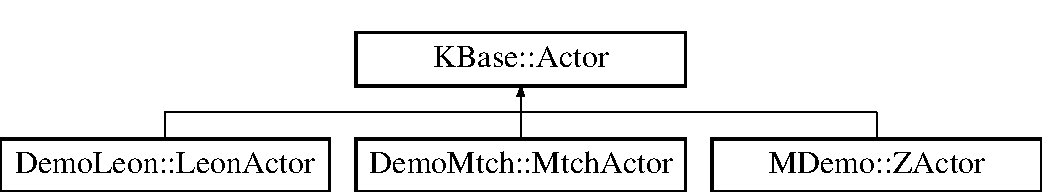
\includegraphics[height=2.000000cm]{class_k_base_1_1_actor}
\end{center}
\end{figure}
\subsection*{Public Member Functions}
\begin{DoxyCompactItemize}
\item 
\hypertarget{class_k_base_1_1_actor_aa1c1b27eea39d8f6d4880956dbb84e0c}{{\bfseries Actor} (string n, string d)}\label{class_k_base_1_1_actor_aa1c1b27eea39d8f6d4880956dbb84e0c}

\item 
\hypertarget{class_k_base_1_1_actor_a4b2e4d5d1e01cd57cfd9838cb4903b31}{virtual double {\bfseries vote} (unsigned int p1, unsigned int p2, const \hyperlink{class_k_base_1_1_state}{State} $\ast$st) const =0}\label{class_k_base_1_1_actor_a4b2e4d5d1e01cd57cfd9838cb4903b31}

\end{DoxyCompactItemize}
\subsection*{Static Public Member Functions}
\begin{DoxyCompactItemize}
\item 
\hypertarget{class_k_base_1_1_actor_a8009ca163b06a0ed5887d49b2b2b552f}{static double {\bfseries third\-Party\-Vote\-S\-U} (double wk, Voting\-Rule vr, Third\-Party\-Commit comm, double pik, double pjk, double uki, double ukj, double ukk)}\label{class_k_base_1_1_actor_a8009ca163b06a0ed5887d49b2b2b552f}

\item 
\hypertarget{class_k_base_1_1_actor_acaff87e7fbc1a74824c61012039e7cc5}{static double {\bfseries v\-Prob\-Little} (Voting\-Rule vr, double wn, double uni, double unj, double contrib\-\_\-i\-\_\-ij, double contrib\-\_\-j\-\_\-ij)}\label{class_k_base_1_1_actor_acaff87e7fbc1a74824c61012039e7cc5}

\end{DoxyCompactItemize}
\subsection*{Public Attributes}
\begin{DoxyCompactItemize}
\item 
\hypertarget{class_k_base_1_1_actor_abbb5242ce42cc3982d0c14eed3cac8d7}{string {\bfseries name} = \char`\"{}G\-A\char`\"{}}\label{class_k_base_1_1_actor_abbb5242ce42cc3982d0c14eed3cac8d7}

\item 
\hypertarget{class_k_base_1_1_actor_a88f1b91e10499b9868f3640b48421e2e}{string {\bfseries desc} = \char`\"{}Generic \hyperlink{class_k_base_1_1_actor}{Actor}\char`\"{}}\label{class_k_base_1_1_actor_a88f1b91e10499b9868f3640b48421e2e}

\end{DoxyCompactItemize}


The documentation for this class was generated from the following files\-:\begin{DoxyCompactItemize}
\item 
kmodel.\-h\item 
kmodel.\-cpp\end{DoxyCompactItemize}

\hypertarget{class_tetris_1_1_board}{\section{Tetris\-:\-:Board Class Reference}
\label{class_tetris_1_1_board}\index{Tetris\-::\-Board@{Tetris\-::\-Board}}
}
Inheritance diagram for Tetris\-:\-:Board\-:\begin{figure}[H]
\begin{center}
\leavevmode
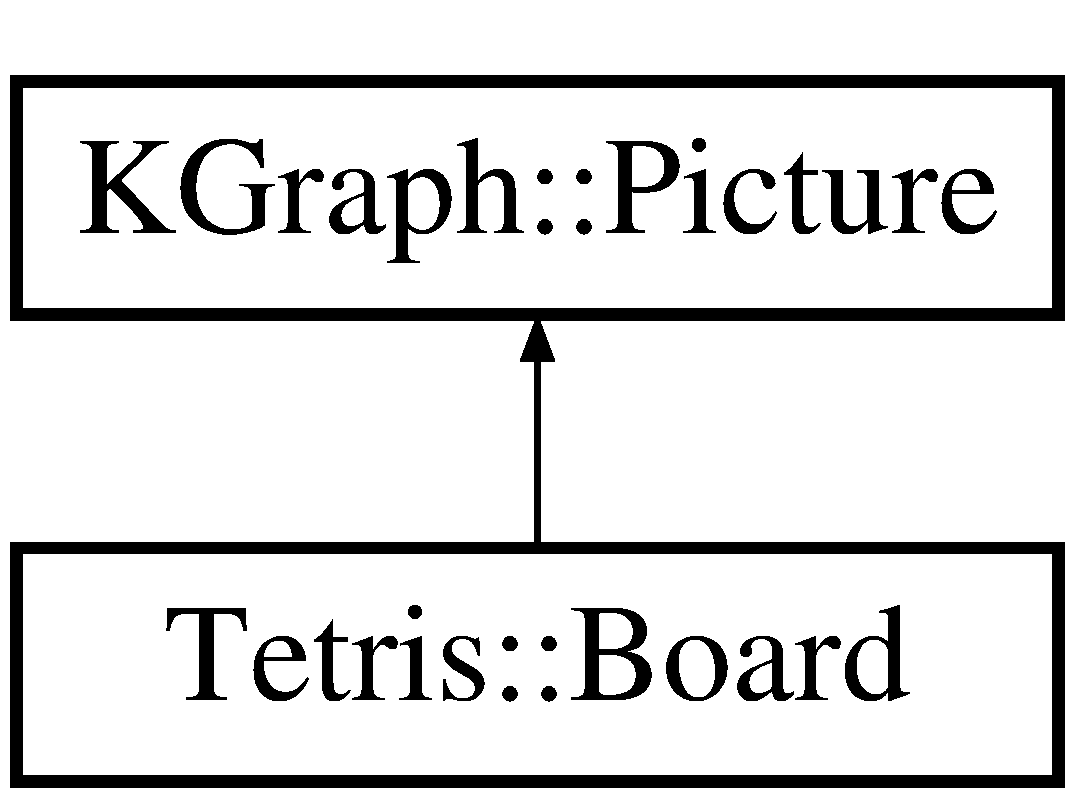
\includegraphics[height=2.000000cm]{class_tetris_1_1_board}
\end{center}
\end{figure}
\subsection*{Public Member Functions}
\begin{DoxyCompactItemize}
\item 
\hypertarget{class_tetris_1_1_board_a6787fe58bbfb7bcc7400efee29fb47ce}{{\bfseries Board} (unsigned int r, unsigned int c)}\label{class_tetris_1_1_board_a6787fe58bbfb7bcc7400efee29fb47ce}

\item 
\hypertarget{class_tetris_1_1_board_afe329c740af93e18f2590b17144ca835}{void {\bfseries randomize\-Fragments} (double f)}\label{class_tetris_1_1_board_afe329c740af93e18f2590b17144ca835}

\item 
\hypertarget{class_tetris_1_1_board_ab76b3272487da487860a40515f15ac6e}{void {\bfseries rotate\-Down} ()}\label{class_tetris_1_1_board_ab76b3272487da487860a40515f15ac6e}

\item 
\hypertarget{class_tetris_1_1_board_a4e07300bd30650055a6cdaf22d57da4f}{virtual void {\bfseries update} (\hyperlink{class_k_graph_1_1_canvas}{Canvas} $\ast$c) const }\label{class_tetris_1_1_board_a4e07300bd30650055a6cdaf22d57da4f}

\item 
\hypertarget{class_tetris_1_1_board_a7700484eab96db9a7495344e1caf8148}{unsigned int {\bfseries n\-From\-I\-J} (int i, int j) const }\label{class_tetris_1_1_board_a7700484eab96db9a7495344e1caf8148}

\item 
\hypertarget{class_tetris_1_1_board_a84807d05f925421a57583f32d6bd6597}{bool {\bfseries reset\-Curr\-Piece} ()}\label{class_tetris_1_1_board_a84807d05f925421a57583f32d6bd6597}

\item 
\hypertarget{class_tetris_1_1_board_a307d7ec8e765ffb6fde1803569062d7a}{unsigned int {\bfseries clear\-Lines} ()}\label{class_tetris_1_1_board_a307d7ec8e765ffb6fde1803569062d7a}

\item 
\hypertarget{class_tetris_1_1_board_aab0b1b4cf3640addf3d7428d9e0c9f36}{unsigned int {\bfseries step\-Game} ()}\label{class_tetris_1_1_board_aab0b1b4cf3640addf3d7428d9e0c9f36}

\item 
\hypertarget{class_tetris_1_1_board_a346f054640b8f39269b092554052e709}{bool {\bfseries try\-L\-Rot} ()}\label{class_tetris_1_1_board_a346f054640b8f39269b092554052e709}

\item 
\hypertarget{class_tetris_1_1_board_a6cac2a0561c0dbe332559e372bd65990}{bool {\bfseries try\-R\-Rot} ()}\label{class_tetris_1_1_board_a6cac2a0561c0dbe332559e372bd65990}

\item 
\hypertarget{class_tetris_1_1_board_a8b0e27172ecd733b30c57d2b8d62a79e}{bool {\bfseries try\-L\-Move} ()}\label{class_tetris_1_1_board_a8b0e27172ecd733b30c57d2b8d62a79e}

\item 
\hypertarget{class_tetris_1_1_board_a8308cf4cad8969c27f660a93e6ebccc5}{bool {\bfseries try\-R\-Move} ()}\label{class_tetris_1_1_board_a8308cf4cad8969c27f660a93e6ebccc5}

\item 
\hypertarget{class_tetris_1_1_board_a48a776d34586af48fa49f337d9028567}{bool {\bfseries test\-S\-Drop} ()}\label{class_tetris_1_1_board_a48a776d34586af48fa49f337d9028567}

\item 
\hypertarget{class_tetris_1_1_board_a7f3ea2560b28333dc9193f346069532c}{bool {\bfseries try\-S\-Drop} ()}\label{class_tetris_1_1_board_a7f3ea2560b28333dc9193f346069532c}

\item 
\hypertarget{class_tetris_1_1_board_ab58e0d33d099c01a9445ce7e72de9d6e}{bool {\bfseries try\-H\-Drop} ()}\label{class_tetris_1_1_board_ab58e0d33d099c01a9445ce7e72de9d6e}

\item 
\hypertarget{class_tetris_1_1_board_adf8407d0a75188dc8c520555803bc92e}{void {\bfseries draw\-Shape} (int i, int j, \hyperlink{class_k_graph_1_1_canvas}{Canvas} $\ast$cnvs) const }\label{class_tetris_1_1_board_adf8407d0a75188dc8c520555803bc92e}

\item 
\hypertarget{class_tetris_1_1_board_a2a314e0a0277a3990a70faa15e8ef7ce}{void {\bfseries draw\-Unit\-Square} (Fl\-\_\-\-Color clr1, int i, int j, bool dot\-P, Fl\-\_\-\-Color clr2, \hyperlink{class_k_graph_1_1_canvas}{Canvas} $\ast$cnvs) const }\label{class_tetris_1_1_board_a2a314e0a0277a3990a70faa15e8ef7ce}

\end{DoxyCompactItemize}
\subsection*{Public Attributes}
\begin{DoxyCompactItemize}
\item 
\hypertarget{class_tetris_1_1_board_a3a2ceec07ee26bb7cc557cb6f7475d65}{unsigned int {\bfseries rows} = 0}\label{class_tetris_1_1_board_a3a2ceec07ee26bb7cc557cb6f7475d65}

\item 
\hypertarget{class_tetris_1_1_board_a969da8e79612f5a2c0ceca875dce6a5f}{unsigned int {\bfseries clms} = 0}\label{class_tetris_1_1_board_a969da8e79612f5a2c0ceca875dce6a5f}

\item 
\hypertarget{class_tetris_1_1_board_ae54353a26b75b00a0d4a7df2ffb6d00c}{\hyperlink{class_tetris_1_1_shape}{Shape} {\bfseries curr\-Shape} = \hyperlink{class_tetris_1_1_shape}{Shape}()}\label{class_tetris_1_1_board_ae54353a26b75b00a0d4a7df2ffb6d00c}

\item 
\hypertarget{class_tetris_1_1_board_a48bb98c9ee351c0af245117d258c5117}{int {\bfseries curr\-I} = 0}\label{class_tetris_1_1_board_a48bb98c9ee351c0af245117d258c5117}

\item 
\hypertarget{class_tetris_1_1_board_a8fb16495579e8b8a3c2fbe695b69ba1a}{int {\bfseries curr\-J} = 0}\label{class_tetris_1_1_board_a8fb16495579e8b8a3c2fbe695b69ba1a}

\item 
\hypertarget{class_tetris_1_1_board_a8ff99e6ca0dfe954f419be4e412a0fc0}{\hyperlink{class_tetris_1_1_shape}{Shape} {\bfseries next\-Shape} = \hyperlink{class_tetris_1_1_shape}{Shape}()}\label{class_tetris_1_1_board_a8ff99e6ca0dfe954f419be4e412a0fc0}

\end{DoxyCompactItemize}
\subsection*{Protected Member Functions}
\begin{DoxyCompactItemize}
\item 
\hypertarget{class_tetris_1_1_board_a4419e7a6fb6393bf70c7f4408bb12788}{void {\bfseries draw\-Background} (\hyperlink{class_k_graph_1_1_canvas}{Canvas} $\ast$c) const }\label{class_tetris_1_1_board_a4419e7a6fb6393bf70c7f4408bb12788}

\item 
\hypertarget{class_tetris_1_1_board_ac56f1e62be8ed638f8db44b38cb6f461}{void {\bfseries draw\-Curr\-Shape} (\hyperlink{class_k_graph_1_1_canvas}{Canvas} $\ast$c) const }\label{class_tetris_1_1_board_ac56f1e62be8ed638f8db44b38cb6f461}

\item 
\hypertarget{class_tetris_1_1_board_ac3ef5641939942570f4a3af634580787}{void {\bfseries draw\-Fragments} (\hyperlink{class_k_graph_1_1_canvas}{Canvas} $\ast$c) const }\label{class_tetris_1_1_board_ac3ef5641939942570f4a3af634580787}

\item 
\hypertarget{class_tetris_1_1_board_ab3709642b6353b7be37d12ed269700fa}{bool {\bfseries test\-Shape} (\hyperlink{class_tetris_1_1_shape}{Shape} s, int i, int j) const }\label{class_tetris_1_1_board_ab3709642b6353b7be37d12ed269700fa}

\item 
\hypertarget{class_tetris_1_1_board_a6a56a0feb6b93238cf6aa1de607ccafd}{void {\bfseries randomize\-Row} (unsigned int i)}\label{class_tetris_1_1_board_a6a56a0feb6b93238cf6aa1de607ccafd}

\item 
\hypertarget{class_tetris_1_1_board_a062ead1d4baae81c85199e0975496717}{vector$<$ T\-Code $>$ {\bfseries empty\-Board} () const }\label{class_tetris_1_1_board_a062ead1d4baae81c85199e0975496717}

\item 
\hypertarget{class_tetris_1_1_board_a1f79463c8f6cfbc45645ea2f33af9760}{void {\bfseries place\-Shape} (\hyperlink{class_tetris_1_1_shape}{Shape} s, int i, int j)}\label{class_tetris_1_1_board_a1f79463c8f6cfbc45645ea2f33af9760}

\item 
\hypertarget{class_tetris_1_1_board_a3fd98c37754dd14b9068716f10661b07}{bool {\bfseries clear\-One\-Line} (const unsigned int i)}\label{class_tetris_1_1_board_a3fd98c37754dd14b9068716f10661b07}

\end{DoxyCompactItemize}
\subsection*{Additional Inherited Members}


The documentation for this class was generated from the following files\-:\begin{DoxyCompactItemize}
\item 
board.\-h\item 
board.\-cpp\end{DoxyCompactItemize}

\hypertarget{class_k_graph_1_1_canvas}{\section{K\-Graph\-:\-:Canvas Class Reference}
\label{class_k_graph_1_1_canvas}\index{K\-Graph\-::\-Canvas@{K\-Graph\-::\-Canvas}}
}
Inheritance diagram for K\-Graph\-:\-:Canvas\-:\begin{figure}[H]
\begin{center}
\leavevmode
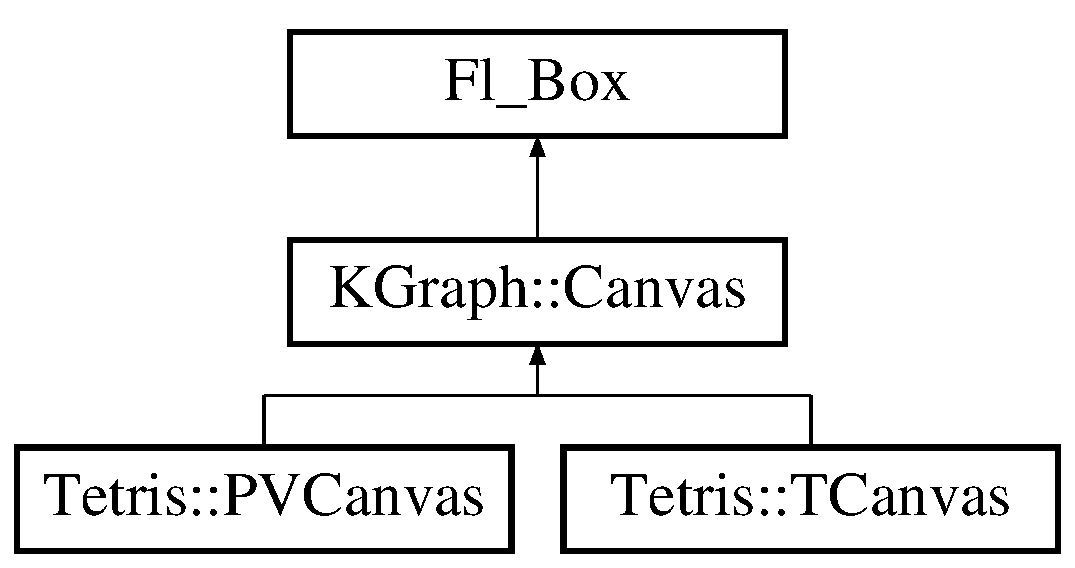
\includegraphics[height=3.000000cm]{class_k_graph_1_1_canvas}
\end{center}
\end{figure}
\subsection*{Public Member Functions}
\begin{DoxyCompactItemize}
\item 
\hypertarget{class_k_graph_1_1_canvas_a6e7e21ab94aed8a2229210bd862f3298}{\hyperlink{class_k_graph_1_1_canvas_a6e7e21ab94aed8a2229210bd862f3298}{Canvas} (int x, int y, int w, int h, const char $\ast$l=0)}\label{class_k_graph_1_1_canvas_a6e7e21ab94aed8a2229210bd862f3298}

\begin{DoxyCompactList}\small\item\em Abstract base class. \end{DoxyCompactList}\item 
\hypertarget{class_k_graph_1_1_canvas_a3454ffa401842bbb52db23ce81e93c93}{void {\bfseries end} ()}\label{class_k_graph_1_1_canvas_a3454ffa401842bbb52db23ce81e93c93}

\item 
\hypertarget{class_k_graph_1_1_canvas_adf47fbb0193ffd33b2ac1cfe69af3265}{void {\bfseries update\-Maps} ()}\label{class_k_graph_1_1_canvas_adf47fbb0193ffd33b2ac1cfe69af3265}

\item 
\hypertarget{class_k_graph_1_1_canvas_a359fd01cf0e9a15cd004174171db1797}{void {\bfseries clear\-Maps} ()}\label{class_k_graph_1_1_canvas_a359fd01cf0e9a15cd004174171db1797}

\item 
\hypertarget{class_k_graph_1_1_canvas_a3723e416805ca1be1fae4eaef0c209aa}{virtual int {\bfseries handle} (int ev)}\label{class_k_graph_1_1_canvas_a3723e416805ca1be1fae4eaef0c209aa}

\item 
\hypertarget{class_k_graph_1_1_canvas_a145097be6a31ee51000bd709acadf225}{virtual void {\bfseries on\-Move} (int x, int y)}\label{class_k_graph_1_1_canvas_a145097be6a31ee51000bd709acadf225}

\item 
\hypertarget{class_k_graph_1_1_canvas_acd9041f3b5119ba11f83ab0359437b39}{virtual void {\bfseries on\-Drag} (int x, int y)}\label{class_k_graph_1_1_canvas_acd9041f3b5119ba11f83ab0359437b39}

\item 
\hypertarget{class_k_graph_1_1_canvas_aff6a255173f26c4de302877acaa6e69b}{virtual void {\bfseries on\-Push} (int x, int y, int b)}\label{class_k_graph_1_1_canvas_aff6a255173f26c4de302877acaa6e69b}

\item 
\hypertarget{class_k_graph_1_1_canvas_a69ac263cd993ab4d70e65d08d60e42c6}{virtual void {\bfseries on\-Release} (int x, int y, int b)}\label{class_k_graph_1_1_canvas_a69ac263cd993ab4d70e65d08d60e42c6}

\item 
\hypertarget{class_k_graph_1_1_canvas_af23da9aa1c998b3902322615775095e0}{virtual void {\bfseries on\-Key\-Down} (int x, int y, int k)}\label{class_k_graph_1_1_canvas_af23da9aa1c998b3902322615775095e0}

\end{DoxyCompactItemize}
\subsection*{Public Attributes}
\begin{DoxyCompactItemize}
\item 
\hypertarget{class_k_graph_1_1_canvas_ad91bab653c0812f5ec606b378246f333}{\hyperlink{class_k_graph_1_1_picture}{Picture} $\ast$ {\bfseries pict} = nullptr}\label{class_k_graph_1_1_canvas_ad91bab653c0812f5ec606b378246f333}

\item 
\hypertarget{class_k_graph_1_1_canvas_aff8c683aefb248d19d72670ba3517bb6}{\hyperlink{class_k_graph_1_1_coord_map}{Coord\-Map} $\ast$ {\bfseries x\-Map} = nullptr}\label{class_k_graph_1_1_canvas_aff8c683aefb248d19d72670ba3517bb6}

\item 
\hypertarget{class_k_graph_1_1_canvas_a51397d902fd8cadfd16f0e42cddfc269}{\hyperlink{class_k_graph_1_1_coord_map}{Coord\-Map} $\ast$ {\bfseries y\-Map} = nullptr}\label{class_k_graph_1_1_canvas_a51397d902fd8cadfd16f0e42cddfc269}

\end{DoxyCompactItemize}


The documentation for this class was generated from the following files\-:\begin{DoxyCompactItemize}
\item 
kgraph.\-h\item 
kgraph.\-cpp\end{DoxyCompactItemize}

\hypertarget{class_tetris_1_1_control_state}{\section{Tetris\-:\-:Control\-State Class Reference}
\label{class_tetris_1_1_control_state}\index{Tetris\-::\-Control\-State@{Tetris\-::\-Control\-State}}
}
\subsection*{Public Member Functions}
\begin{DoxyCompactItemize}
\item 
\hypertarget{class_tetris_1_1_control_state_aa5acf647f5feac932c4b96a9691d366e}{{\bfseries Control\-State} (unsigned int bv, unsigned int pv, unsigned int gv, unsigned int rv)}\label{class_tetris_1_1_control_state_aa5acf647f5feac932c4b96a9691d366e}

\end{DoxyCompactItemize}
\subsection*{Public Attributes}
\begin{DoxyCompactItemize}
\item 
\hypertarget{class_tetris_1_1_control_state_a812b12ec2dbde3252cd46fee68852144}{unsigned int {\bfseries bg} = 1}\label{class_tetris_1_1_control_state_a812b12ec2dbde3252cd46fee68852144}

\item 
\hypertarget{class_tetris_1_1_control_state_aa2755dfd1afa1fbee79302a15aed385a}{unsigned int {\bfseries pc} = 2}\label{class_tetris_1_1_control_state_aa2755dfd1afa1fbee79302a15aed385a}

\item 
\hypertarget{class_tetris_1_1_control_state_a1fb910204a348fd2d4544a383e4049c2}{unsigned int {\bfseries gt} = 1}\label{class_tetris_1_1_control_state_a1fb910204a348fd2d4544a383e4049c2}

\item 
\hypertarget{class_tetris_1_1_control_state_abfe612ad0b21e6f4a429987272c36785}{unsigned int {\bfseries rt} = 0}\label{class_tetris_1_1_control_state_abfe612ad0b21e6f4a429987272c36785}

\end{DoxyCompactItemize}


The documentation for this class was generated from the following file\-:\begin{DoxyCompactItemize}
\item 
tmain.\-h\end{DoxyCompactItemize}

\hypertarget{class_k_graph_1_1_coord_map}{\section{K\-Graph\-:\-:Coord\-Map Class Reference}
\label{class_k_graph_1_1_coord_map}\index{K\-Graph\-::\-Coord\-Map@{K\-Graph\-::\-Coord\-Map}}
}
\subsection*{Public Member Functions}
\begin{DoxyCompactItemize}
\item 
\hypertarget{class_k_graph_1_1_coord_map_a72ac3356e3d53a70c85c486cfc0961b2}{{\bfseries Coord\-Map} (int s1, double d1, int s2, double d2)}\label{class_k_graph_1_1_coord_map_a72ac3356e3d53a70c85c486cfc0961b2}

\item 
\hypertarget{class_k_graph_1_1_coord_map_abcca196bb8f198b296472f2b66ad60c9}{int {\bfseries d2s} (double d)}\label{class_k_graph_1_1_coord_map_abcca196bb8f198b296472f2b66ad60c9}

\item 
\hypertarget{class_k_graph_1_1_coord_map_a80a81e4d1f56ae6e0cb8dfc98bd8eaef}{double {\bfseries s2d} (int s)}\label{class_k_graph_1_1_coord_map_a80a81e4d1f56ae6e0cb8dfc98bd8eaef}

\end{DoxyCompactItemize}
\subsection*{Protected Attributes}
\begin{DoxyCompactItemize}
\item 
\hypertarget{class_k_graph_1_1_coord_map_a654b52c175c737e466bb60f8f9d0da26}{double {\bfseries as} = 0}\label{class_k_graph_1_1_coord_map_a654b52c175c737e466bb60f8f9d0da26}

\item 
\hypertarget{class_k_graph_1_1_coord_map_a5935710ef18e45de6611c37c21c64fec}{double {\bfseries bs} = 0}\label{class_k_graph_1_1_coord_map_a5935710ef18e45de6611c37c21c64fec}

\item 
\hypertarget{class_k_graph_1_1_coord_map_ad0587bf0739d0224f7527a6a4b555ce7}{double {\bfseries ad} = 0}\label{class_k_graph_1_1_coord_map_ad0587bf0739d0224f7527a6a4b555ce7}

\item 
\hypertarget{class_k_graph_1_1_coord_map_a3f2454f1776339ce2edd73d558be286c}{double {\bfseries bd} = 0}\label{class_k_graph_1_1_coord_map_a3f2454f1776339ce2edd73d558be286c}

\end{DoxyCompactItemize}


The documentation for this class was generated from the following files\-:\begin{DoxyCompactItemize}
\item 
kgraph.\-h\item 
kgraph.\-cpp\end{DoxyCompactItemize}

\hypertarget{class_k_base_1_1_e_model}{\section{K\-Base\-:\-:E\-Model$<$ P\-T $>$ Class Template Reference}
\label{class_k_base_1_1_e_model}\index{K\-Base\-::\-E\-Model$<$ P\-T $>$@{K\-Base\-::\-E\-Model$<$ P\-T $>$}}
}
Inheritance diagram for K\-Base\-:\-:E\-Model$<$ P\-T $>$\-:\begin{figure}[H]
\begin{center}
\leavevmode
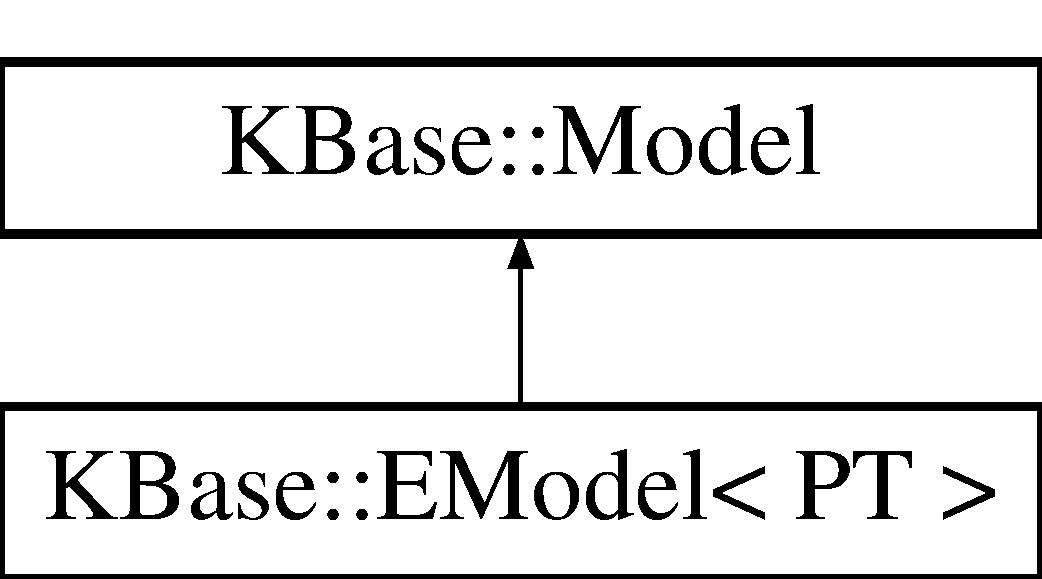
\includegraphics[height=2.000000cm]{class_k_base_1_1_e_model}
\end{center}
\end{figure}
\subsection*{Public Member Functions}
\begin{DoxyCompactItemize}
\item 
\hypertarget{class_k_base_1_1_e_model_ac8acff3476069856a092599f797046f8}{{\bfseries E\-Model} (\hyperlink{class_k_base_1_1_p_r_n_g}{P\-R\-N\-G} $\ast$r, string d=\char`\"{}\char`\"{})}\label{class_k_base_1_1_e_model_ac8acff3476069856a092599f797046f8}

\item 
\hypertarget{class_k_base_1_1_e_model_aca2a35d8e8f23000a47e4d92fce26690}{void {\bfseries set\-Options} ()}\label{class_k_base_1_1_e_model_aca2a35d8e8f23000a47e4d92fce26690}

\item 
\hypertarget{class_k_base_1_1_e_model_a19063b42bcf8aa958684c2fe5eca04b7}{unsigned int {\bfseries num\-Options} () const }\label{class_k_base_1_1_e_model_a19063b42bcf8aa958684c2fe5eca04b7}

\item 
\hypertarget{class_k_base_1_1_e_model_a74f1728c3983329b50bec0deb484d366}{P\-T $\ast$ {\bfseries nth\-Option} (unsigned int i) const }\label{class_k_base_1_1_e_model_a74f1728c3983329b50bec0deb484d366}

\end{DoxyCompactItemize}
\subsection*{Public Attributes}
\begin{DoxyCompactItemize}
\item 
\hypertarget{class_k_base_1_1_e_model_ad117e0f01142f5a9beb4353145eb31f7}{function$<$ vector$<$ P\-T $\ast$ $>$)$>$ {\bfseries enum\-Options} = nullptr}\label{class_k_base_1_1_e_model_ad117e0f01142f5a9beb4353145eb31f7}

\end{DoxyCompactItemize}
\subsection*{Protected Attributes}
\begin{DoxyCompactItemize}
\item 
\hypertarget{class_k_base_1_1_e_model_afd8349b62c23c8d390f5911951365592}{vector$<$ P\-T $\ast$ $>$ {\bfseries theta} = \{\}}\label{class_k_base_1_1_e_model_afd8349b62c23c8d390f5911951365592}

\end{DoxyCompactItemize}
\subsection*{Additional Inherited Members}


The documentation for this class was generated from the following files\-:\begin{DoxyCompactItemize}
\item 
emodel.\-h\item 
emodel.\-cpp\end{DoxyCompactItemize}

\hypertarget{class_k_base_1_1_e_position}{\section{K\-Base\-:\-:E\-Position$<$ P\-T $>$ Class Template Reference}
\label{class_k_base_1_1_e_position}\index{K\-Base\-::\-E\-Position$<$ P\-T $>$@{K\-Base\-::\-E\-Position$<$ P\-T $>$}}
}
Inheritance diagram for K\-Base\-:\-:E\-Position$<$ P\-T $>$\-:\begin{figure}[H]
\begin{center}
\leavevmode
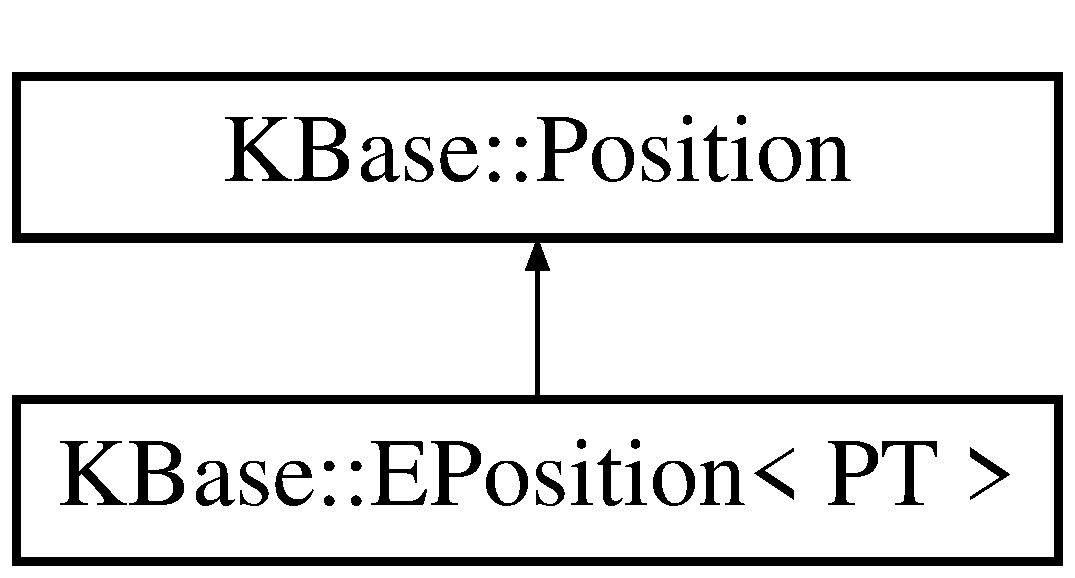
\includegraphics[height=2.000000cm]{class_k_base_1_1_e_position}
\end{center}
\end{figure}
\subsection*{Public Member Functions}
\begin{DoxyCompactItemize}
\item 
\hypertarget{class_k_base_1_1_e_position_a0710d98dde1e1582239699621a6b97aa}{{\bfseries E\-Position} (\hyperlink{class_k_base_1_1_e_model}{E\-Model}$<$ P\-T $>$ $\ast$m, int n)}\label{class_k_base_1_1_e_position_a0710d98dde1e1582239699621a6b97aa}

\end{DoxyCompactItemize}
\subsection*{Protected Attributes}
\begin{DoxyCompactItemize}
\item 
\hypertarget{class_k_base_1_1_e_position_adcf829a42e8b732d69dea75a0e4476c8}{\hyperlink{class_k_base_1_1_e_model}{E\-Model}$<$ P\-T $>$ $\ast$ {\bfseries e\-Mod} = nullptr}\label{class_k_base_1_1_e_position_adcf829a42e8b732d69dea75a0e4476c8}

\item 
\hypertarget{class_k_base_1_1_e_position_a3e8046ec0148d120946072fee775e895}{int {\bfseries ndx} = -\/1}\label{class_k_base_1_1_e_position_a3e8046ec0148d120946072fee775e895}

\end{DoxyCompactItemize}
\subsection*{Additional Inherited Members}


The documentation for this class was generated from the following files\-:\begin{DoxyCompactItemize}
\item 
emodel.\-h\item 
emodel.\-cpp\end{DoxyCompactItemize}

\hypertarget{class_k_base_1_1_e_state}{\section{K\-Base\-:\-:E\-State$<$ P\-T $>$ Class Template Reference}
\label{class_k_base_1_1_e_state}\index{K\-Base\-::\-E\-State$<$ P\-T $>$@{K\-Base\-::\-E\-State$<$ P\-T $>$}}
}
Inheritance diagram for K\-Base\-:\-:E\-State$<$ P\-T $>$\-:\begin{figure}[H]
\begin{center}
\leavevmode
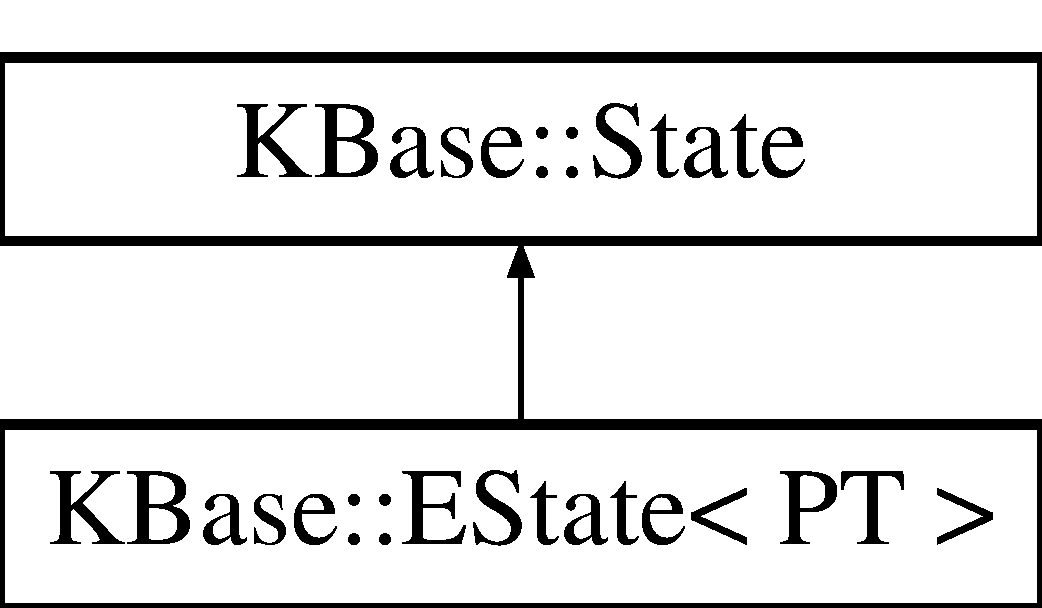
\includegraphics[height=2.000000cm]{class_k_base_1_1_e_state}
\end{center}
\end{figure}
\subsection*{Public Member Functions}
\begin{DoxyCompactItemize}
\item 
\hypertarget{class_k_base_1_1_e_state_a9cd7e7f73e08e06b0bd3658ba7891c3f}{{\bfseries E\-State} (\hyperlink{class_k_base_1_1_e_model}{E\-Model}$<$ P\-T $>$ $\ast$mod)}\label{class_k_base_1_1_e_state_a9cd7e7f73e08e06b0bd3658ba7891c3f}

\item 
\hypertarget{class_k_base_1_1_e_state_aa00dab6c3b68754448e0866952c4e057}{void {\bfseries set\-Values} ()}\label{class_k_base_1_1_e_state_aa00dab6c3b68754448e0866952c4e057}

\end{DoxyCompactItemize}
\subsection*{Protected Member Functions}
\begin{DoxyCompactItemize}
\item 
\hypertarget{class_k_base_1_1_e_state_a419573f5f256e4979fa830af21121e3b}{void {\bfseries set\-All\-A\-Util} (Reporting\-Level rl)}\label{class_k_base_1_1_e_state_a419573f5f256e4979fa830af21121e3b}

\end{DoxyCompactItemize}
\subsection*{Protected Attributes}
\begin{DoxyCompactItemize}
\item 
\hypertarget{class_k_base_1_1_e_state_acc31eed9873f571e46d369c27c08f67d}{function$<$ vector$<$ \hyperlink{class_k_base_1_1_k_matrix}{K\-Matrix} $>$)$>$ {\bfseries get\-A\-Utils} = nullptr}\label{class_k_base_1_1_e_state_acc31eed9873f571e46d369c27c08f67d}

\item 
\hypertarget{class_k_base_1_1_e_state_ac71ef963eb875e2ff6786fb78751d6eb}{function$<$ vector$<$ double $>$\\*
unsigned int j, const \hyperlink{class_k_base_1_1_e_model}{E\-Model}\\*
$<$ P\-T $>$ $\ast$)$>$ {\bfseries actor\-V\-Fn} = nullptr}\label{class_k_base_1_1_e_state_ac71ef963eb875e2ff6786fb78751d6eb}

\end{DoxyCompactItemize}
\subsection*{Additional Inherited Members}


The documentation for this class was generated from the following files\-:\begin{DoxyCompactItemize}
\item 
emodel.\-h\item 
emodel.\-cpp\end{DoxyCompactItemize}

\hypertarget{class_k_base_1_1_g_a_opt}{\section{K\-Base\-:\-:G\-A\-Opt$<$ G\-A\-P $>$ Class Template Reference}
\label{class_k_base_1_1_g_a_opt}\index{K\-Base\-::\-G\-A\-Opt$<$ G\-A\-P $>$@{K\-Base\-::\-G\-A\-Opt$<$ G\-A\-P $>$}}
}
\subsection*{Public Member Functions}
\begin{DoxyCompactItemize}
\item 
\hypertarget{class_k_base_1_1_g_a_opt_a5f67a17ba318dd9a65c0a66c951fa1a2}{{\bfseries G\-A\-Opt} (unsigned int s)}\label{class_k_base_1_1_g_a_opt_a5f67a17ba318dd9a65c0a66c951fa1a2}

\item 
\hypertarget{class_k_base_1_1_g_a_opt_adcc44debffd7f234863719a1b4617130}{void {\bfseries init} (vector$<$ G\-A\-P $\ast$ $>$ ipop)}\label{class_k_base_1_1_g_a_opt_adcc44debffd7f234863719a1b4617130}

\item 
\hypertarget{class_k_base_1_1_g_a_opt_ad352dc1d49da8261c5a6928418a363c9}{void {\bfseries fill} (\hyperlink{class_k_base_1_1_p_r_n_g}{P\-R\-N\-G} $\ast$rng)}\label{class_k_base_1_1_g_a_opt_ad352dc1d49da8261c5a6928418a363c9}

\item 
\hypertarget{class_k_base_1_1_g_a_opt_a3b64c759cdcdf165e49aa3f5a271a434}{void {\bfseries run} (\hyperlink{class_k_base_1_1_p_r_n_g}{P\-R\-N\-G} $\ast$rng, double c, double m, unsigned int max\-I, double s\-Th, unsigned int max\-S, Reporting\-Level srl, unsigned int \&iter, unsigned int \&s\-Iter)}\label{class_k_base_1_1_g_a_opt_a3b64c759cdcdf165e49aa3f5a271a434}

\item 
\hypertarget{class_k_base_1_1_g_a_opt_a6e9ae733023e9b70878b1d4051d0ce56}{tuple$<$ double, G\-A\-P $\ast$ $>$ {\bfseries get\-Nth} (unsigned int n)}\label{class_k_base_1_1_g_a_opt_a6e9ae733023e9b70878b1d4051d0ce56}

\item 
\hypertarget{class_k_base_1_1_g_a_opt_ad7a00c54ac150ff23238f4daaaea7b98}{void {\bfseries show} ()}\label{class_k_base_1_1_g_a_opt_ad7a00c54ac150ff23238f4daaaea7b98}

\item 
\hypertarget{class_k_base_1_1_g_a_opt_aaee74f8e07ff31a763a55d0f7f8a3356}{void {\bfseries sort\-Pop} ()}\label{class_k_base_1_1_g_a_opt_aaee74f8e07ff31a763a55d0f7f8a3356}

\end{DoxyCompactItemize}
\subsection*{Public Attributes}
\begin{DoxyCompactItemize}
\item 
\hypertarget{class_k_base_1_1_g_a_opt_aee09bf0ec409419f10fff73ca8a31224}{function$<$ tuple$<$ G\-A\-P $\ast$, G\-A\-P $\ast$ $>$\\*
const G\-A\-P $\ast$g1, const G\-A\-P $\ast$g2, \\*
\hyperlink{class_k_base_1_1_p_r_n_g}{P\-R\-N\-G} $\ast$rng)$>$ {\bfseries cross} = nullptr}\label{class_k_base_1_1_g_a_opt_aee09bf0ec409419f10fff73ca8a31224}

\item 
\hypertarget{class_k_base_1_1_g_a_opt_a6e1ecad6a7ccb08d4b70e7e9c1fd04f4}{function$<$ G\-A\-P $\ast$(const G\-A\-P $\ast$g1, \\*
\hyperlink{class_k_base_1_1_p_r_n_g}{P\-R\-N\-G} $\ast$rng)$>$ {\bfseries mutate} = nullptr}\label{class_k_base_1_1_g_a_opt_a6e1ecad6a7ccb08d4b70e7e9c1fd04f4}

\item 
\hypertarget{class_k_base_1_1_g_a_opt_a03bc51aac124db77e9b88889abbaebbe}{function$<$ double(const G\-A\-P $\ast$g1)$>$ {\bfseries eval} = nullptr}\label{class_k_base_1_1_g_a_opt_a03bc51aac124db77e9b88889abbaebbe}

\item 
\hypertarget{class_k_base_1_1_g_a_opt_ac4a251e61b6daafe83ded6f956e05100}{function$<$ void(const G\-A\-P $\ast$)$>$ {\bfseries show\-Gene} = nullptr}\label{class_k_base_1_1_g_a_opt_ac4a251e61b6daafe83ded6f956e05100}

\item 
\hypertarget{class_k_base_1_1_g_a_opt_a2af02819c506af8a17d595a0fd20dee1}{function$<$ G\-A\-P $\ast$(\hyperlink{class_k_base_1_1_p_r_n_g}{P\-R\-N\-G} $\ast$rng)$>$ {\bfseries make\-Gene} = nullptr}\label{class_k_base_1_1_g_a_opt_a2af02819c506af8a17d595a0fd20dee1}

\item 
\hypertarget{class_k_base_1_1_g_a_opt_afde428b2ce65402d7ca6d9bffdc23299}{function$<$ bool(const G\-A\-P $\ast$g1, \\*
const G\-A\-P $\ast$g2)$>$ {\bfseries equiv} = nullptr}\label{class_k_base_1_1_g_a_opt_afde428b2ce65402d7ca6d9bffdc23299}

\end{DoxyCompactItemize}
\subsection*{Protected Member Functions}
\begin{DoxyCompactItemize}
\item 
\hypertarget{class_k_base_1_1_g_a_opt_a1f92c5390aa9398a58ea6f6b0f4640dd}{void {\bfseries step} ()}\label{class_k_base_1_1_g_a_opt_a1f92c5390aa9398a58ea6f6b0f4640dd}

\item 
\hypertarget{class_k_base_1_1_g_a_opt_af300a4b2be804e4173480bae2f2ea002}{void {\bfseries mutate\-Pop} ()}\label{class_k_base_1_1_g_a_opt_af300a4b2be804e4173480bae2f2ea002}

\item 
\hypertarget{class_k_base_1_1_g_a_opt_a99312a5f465ffc92f28d25d42f41217f}{void {\bfseries cross\-Pop} ()}\label{class_k_base_1_1_g_a_opt_a99312a5f465ffc92f28d25d42f41217f}

\item 
\hypertarget{class_k_base_1_1_g_a_opt_af145546dafca23061d112cbaa1d5d004}{void {\bfseries drop\-Dups} ()}\label{class_k_base_1_1_g_a_opt_af145546dafca23061d112cbaa1d5d004}

\item 
\hypertarget{class_k_base_1_1_g_a_opt_a7ea4d2e234ab37149e104f0238bbefda}{void {\bfseries select\-Pop} ()}\label{class_k_base_1_1_g_a_opt_a7ea4d2e234ab37149e104f0238bbefda}

\item 
\hypertarget{class_k_base_1_1_g_a_opt_adaf83b9b8c59840fbbf40b4d928952a2}{G\-A\-P $\ast$ {\bfseries mutate\-One} (const G\-A\-P $\ast$g1, \hyperlink{class_k_base_1_1_p_r_n_g}{P\-R\-N\-G} $\ast$rng)}\label{class_k_base_1_1_g_a_opt_adaf83b9b8c59840fbbf40b4d928952a2}

\item 
\hypertarget{class_k_base_1_1_g_a_opt_aefff59e83d40ab47d20a0866db05d25b}{tuple$<$ G\-A\-P $\ast$, G\-A\-P $\ast$ $>$ {\bfseries cross\-Pair} (const G\-A\-P $\ast$g1, const G\-A\-P $\ast$g2, \hyperlink{class_k_base_1_1_p_r_n_g}{P\-R\-N\-G} $\ast$rng)}\label{class_k_base_1_1_g_a_opt_aefff59e83d40ab47d20a0866db05d25b}

\item 
\hypertarget{class_k_base_1_1_g_a_opt_ae9a4bcd82674244186378250ab4fafc0}{void {\bfseries cyclic\-Apply} (function$<$ void(unsigned int i)$>$ fn, double f)}\label{class_k_base_1_1_g_a_opt_ae9a4bcd82674244186378250ab4fafc0}

\end{DoxyCompactItemize}
\subsection*{Protected Attributes}
\begin{DoxyCompactItemize}
\item 
\hypertarget{class_k_base_1_1_g_a_opt_a097887d3de46feca8af4ae6aa3f50bc8}{vector$<$ tuple$<$ double, G\-A\-P $\ast$ $>$ $>$ {\bfseries gpool} = \{\}}\label{class_k_base_1_1_g_a_opt_a097887d3de46feca8af4ae6aa3f50bc8}

\item 
\hypertarget{class_k_base_1_1_g_a_opt_a68568fb8b08bcbd64d1f3e2eebc0704d}{unsigned int {\bfseries p\-Size} = 0}\label{class_k_base_1_1_g_a_opt_a68568fb8b08bcbd64d1f3e2eebc0704d}

\item 
\hypertarget{class_k_base_1_1_g_a_opt_a917bf044a35172f2da70b4f9db57e7d9}{double {\bfseries c\-Frac} = 1.\-0}\label{class_k_base_1_1_g_a_opt_a917bf044a35172f2da70b4f9db57e7d9}

\item 
\hypertarget{class_k_base_1_1_g_a_opt_ab3b5fd83355daa4457ab8b19ddb8b9a9}{double {\bfseries m\-Frac} = 0.\-5}\label{class_k_base_1_1_g_a_opt_ab3b5fd83355daa4457ab8b19ddb8b9a9}

\item 
\hypertarget{class_k_base_1_1_g_a_opt_a62a5c058b06b16fcab01909911a37255}{\hyperlink{class_k_base_1_1_p_r_n_g}{P\-R\-N\-G} $\ast$ {\bfseries rng} = nullptr}\label{class_k_base_1_1_g_a_opt_a62a5c058b06b16fcab01909911a37255}

\end{DoxyCompactItemize}


The documentation for this class was generated from the following file\-:\begin{DoxyCompactItemize}
\item 
gaopt.\-h\end{DoxyCompactItemize}

\hypertarget{class_k_base_1_1_g_h_c_search}{\section{K\-Base\-:\-:G\-H\-C\-Search$<$ H\-C\-P $>$ Class Template Reference}
\label{class_k_base_1_1_g_h_c_search}\index{K\-Base\-::\-G\-H\-C\-Search$<$ H\-C\-P $>$@{K\-Base\-::\-G\-H\-C\-Search$<$ H\-C\-P $>$}}
}
\subsection*{Public Member Functions}
\begin{DoxyCompactItemize}
\item 
\hypertarget{class_k_base_1_1_g_h_c_search_a69f34435e5a5e2c63439bf8e04160a90}{tuple$<$ double, H\-C\-P, unsigned \\*
int, unsigned int $>$ {\bfseries run} (H\-C\-P p0, Reporting\-Level srl, unsigned int i\-Max, unsigned int s\-Max, double s\-Tol)}\label{class_k_base_1_1_g_h_c_search_a69f34435e5a5e2c63439bf8e04160a90}

\end{DoxyCompactItemize}
\subsection*{Public Attributes}
\begin{DoxyCompactItemize}
\item 
\hypertarget{class_k_base_1_1_g_h_c_search_a2fd914dfbcf61a1226c09cec50634f83}{function$<$ double(const H\-C\-P)$>$ {\bfseries eval} = nullptr}\label{class_k_base_1_1_g_h_c_search_a2fd914dfbcf61a1226c09cec50634f83}

\item 
\hypertarget{class_k_base_1_1_g_h_c_search_a8d2f1b18ccc7203763d4ddc7cc7243af}{function$<$ vector$<$ H\-C\-P $>$const H\-C\-P)$>$ {\bfseries nghbrs} = nullptr}\label{class_k_base_1_1_g_h_c_search_a8d2f1b18ccc7203763d4ddc7cc7243af}

\item 
\hypertarget{class_k_base_1_1_g_h_c_search_ac3332b5acb47013165ae3e218f8b658a}{function$<$ void(const H\-C\-P)$>$ {\bfseries show} = nullptr}\label{class_k_base_1_1_g_h_c_search_ac3332b5acb47013165ae3e218f8b658a}

\end{DoxyCompactItemize}


The documentation for this class was generated from the following file\-:\begin{DoxyCompactItemize}
\item 
hcsearch.\-h\end{DoxyCompactItemize}

\hypertarget{class_k_base_1_1_k_exception}{\section{K\-Base\-:\-:K\-Exception Class Reference}
\label{class_k_base_1_1_k_exception}\index{K\-Base\-::\-K\-Exception@{K\-Base\-::\-K\-Exception}}
}
\subsection*{Public Member Functions}
\begin{DoxyCompactItemize}
\item 
\hypertarget{class_k_base_1_1_k_exception_a3bbce941dab9a8e3cc5ae3e747b03c0a}{{\bfseries K\-Exception} (string m)}\label{class_k_base_1_1_k_exception_a3bbce941dab9a8e3cc5ae3e747b03c0a}

\end{DoxyCompactItemize}
\subsection*{Public Attributes}
\begin{DoxyCompactItemize}
\item 
\hypertarget{class_k_base_1_1_k_exception_a92ce81f7caeceffd00dde7dfeea2eb35}{string {\bfseries msg} =\char`\"{}\char`\"{}}\label{class_k_base_1_1_k_exception_a92ce81f7caeceffd00dde7dfeea2eb35}

\end{DoxyCompactItemize}


The documentation for this class was generated from the following files\-:\begin{DoxyCompactItemize}
\item 
kutils.\-h\item 
kutils.\-cpp\end{DoxyCompactItemize}

\hypertarget{class_k_base_1_1_k_matrix}{\section{K\-Base\-:\-:K\-Matrix Class Reference}
\label{class_k_base_1_1_k_matrix}\index{K\-Base\-::\-K\-Matrix@{K\-Base\-::\-K\-Matrix}}
}
Inheritance diagram for K\-Base\-:\-:K\-Matrix\-:\begin{figure}[H]
\begin{center}
\leavevmode
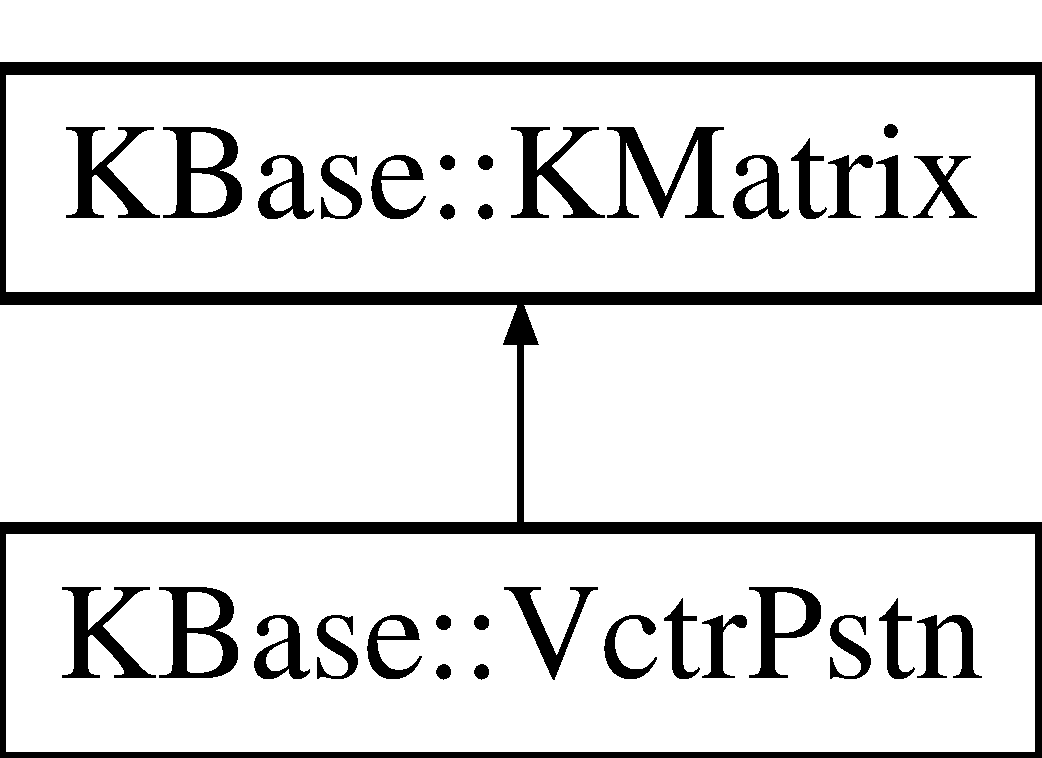
\includegraphics[height=2.000000cm]{class_k_base_1_1_k_matrix}
\end{center}
\end{figure}
\subsection*{Public Member Functions}
\begin{DoxyCompactItemize}
\item 
\hypertarget{class_k_base_1_1_k_matrix_a2cccedf095e532984e75dbd51c9cc7ff}{{\bfseries K\-Matrix} (unsigned int nr, unsigned int nc, double iv=0.\-0)}\label{class_k_base_1_1_k_matrix_a2cccedf095e532984e75dbd51c9cc7ff}

\item 
\hypertarget{class_k_base_1_1_k_matrix_af3985ff0b33b0819275f480cc6b90204}{double {\bfseries operator()} (unsigned int i, unsigned int j) const }\label{class_k_base_1_1_k_matrix_af3985ff0b33b0819275f480cc6b90204}

\item 
\hypertarget{class_k_base_1_1_k_matrix_ada1010a6a9405a3db032d64475798894}{double \& {\bfseries operator()} (unsigned int i, unsigned int j)}\label{class_k_base_1_1_k_matrix_ada1010a6a9405a3db032d64475798894}

\item 
\hypertarget{class_k_base_1_1_k_matrix_ad6bfd476ee5e2370a67739177494f026}{void {\bfseries m\-Printf} (string) const }\label{class_k_base_1_1_k_matrix_ad6bfd476ee5e2370a67739177494f026}

\item 
\hypertarget{class_k_base_1_1_k_matrix_ac6113a035b1e439bb4c26463965f1d88}{unsigned int {\bfseries num\-R} () const }\label{class_k_base_1_1_k_matrix_ac6113a035b1e439bb4c26463965f1d88}

\item 
\hypertarget{class_k_base_1_1_k_matrix_a7c0d998a29889fd746f960061fc44a1f}{unsigned int {\bfseries num\-C} () const }\label{class_k_base_1_1_k_matrix_a7c0d998a29889fd746f960061fc44a1f}

\item 
\hypertarget{class_k_base_1_1_k_matrix_a27e030bc0368bf4ce42f88db592381f3}{vector$<$ double $>$\-::iterator {\bfseries begin} ()}\label{class_k_base_1_1_k_matrix_a27e030bc0368bf4ce42f88db592381f3}

\item 
\hypertarget{class_k_base_1_1_k_matrix_ae0dd848ce08ab94719a1a2e20e6dd1bd}{vector$<$ double $>$\-::iterator {\bfseries end} ()}\label{class_k_base_1_1_k_matrix_ae0dd848ce08ab94719a1a2e20e6dd1bd}

\item 
\hypertarget{class_k_base_1_1_k_matrix_adab9d9e6f5d97055585c43353f7147b9}{vector$<$ double $>$\-::const\-\_\-iterator {\bfseries cbegin} ()}\label{class_k_base_1_1_k_matrix_adab9d9e6f5d97055585c43353f7147b9}

\item 
\hypertarget{class_k_base_1_1_k_matrix_a6ce3854ba4e8d8c4bd7f3c8ba776035f}{vector$<$ double $>$\-::const\-\_\-iterator {\bfseries cend} ()}\label{class_k_base_1_1_k_matrix_a6ce3854ba4e8d8c4bd7f3c8ba776035f}

\item 
\hypertarget{class_k_base_1_1_k_matrix_acdc3441642f9b30b6f60245ebcba19d7}{vector$<$ double $>$\-::const\-\_\-iterator {\bfseries begin} () const }\label{class_k_base_1_1_k_matrix_acdc3441642f9b30b6f60245ebcba19d7}

\item 
\hypertarget{class_k_base_1_1_k_matrix_aa78634fb071c07e3666953ae3d46b5d0}{vector$<$ double $>$\-::const\-\_\-iterator {\bfseries end} () const }\label{class_k_base_1_1_k_matrix_aa78634fb071c07e3666953ae3d46b5d0}

\end{DoxyCompactItemize}
\subsection*{Static Public Member Functions}
\begin{DoxyCompactItemize}
\item 
\hypertarget{class_k_base_1_1_k_matrix_a1dccc21222d9e23d23d8b817f34be1b6}{static \hyperlink{class_k_base_1_1_k_matrix}{K\-Matrix} {\bfseries uniform} (\hyperlink{class_k_base_1_1_p_r_n_g}{P\-R\-N\-G} $\ast$rng, unsigned int nr, unsigned int nc, double a, double b)}\label{class_k_base_1_1_k_matrix_a1dccc21222d9e23d23d8b817f34be1b6}

\item 
\hypertarget{class_k_base_1_1_k_matrix_a71870c0b41f64264b8237b7babe3ef32}{static \hyperlink{class_k_base_1_1_k_matrix}{K\-Matrix} {\bfseries map} (function$<$ double(unsigned int i, unsigned int j)$>$ f, unsigned int nr, unsigned int nc)}\label{class_k_base_1_1_k_matrix_a71870c0b41f64264b8237b7babe3ef32}

\item 
\hypertarget{class_k_base_1_1_k_matrix_a4178571f049c87caa81152ea8ef57f39}{static void {\bfseries map\-V} (function$<$ void(unsigned int i, unsigned int j)$>$ f, unsigned int nr, unsigned int nc)}\label{class_k_base_1_1_k_matrix_a4178571f049c87caa81152ea8ef57f39}

\item 
\hypertarget{class_k_base_1_1_k_matrix_a4b3e5d66773ea8b8e7a39a67a8f28ece}{static \hyperlink{class_k_base_1_1_k_matrix}{K\-Matrix} {\bfseries array\-Init} (const double mv\mbox{[}$\,$\mbox{]}, const unsigned int \&rows, const unsigned int \&clms)}\label{class_k_base_1_1_k_matrix_a4b3e5d66773ea8b8e7a39a67a8f28ece}

\end{DoxyCompactItemize}
\subsection*{Protected Attributes}
\begin{DoxyCompactItemize}
\item 
\hypertarget{class_k_base_1_1_k_matrix_a48c47ae18ab41bb48b47e3c7c6cc5fd5}{unsigned int {\bfseries rows} = 0}\label{class_k_base_1_1_k_matrix_a48c47ae18ab41bb48b47e3c7c6cc5fd5}

\item 
\hypertarget{class_k_base_1_1_k_matrix_ac3a43df2f84481d2cad99768d66c8093}{unsigned int {\bfseries clms} = 0}\label{class_k_base_1_1_k_matrix_ac3a43df2f84481d2cad99768d66c8093}

\item 
\hypertarget{class_k_base_1_1_k_matrix_a04f0e8fddb65b1b481d6ca8f3783fb0d}{vector$<$ double $>$ {\bfseries vals} = vector$<$double$>$()}\label{class_k_base_1_1_k_matrix_a04f0e8fddb65b1b481d6ca8f3783fb0d}

\end{DoxyCompactItemize}
\subsection*{Friends}
\begin{DoxyCompactItemize}
\item 
\hypertarget{class_k_base_1_1_k_matrix_a2113818dcb2a9a07232d94f3f9aa4960}{\hyperlink{class_k_base_1_1_k_matrix}{K\-Matrix} {\bfseries inv} (const \hyperlink{class_k_base_1_1_k_matrix}{K\-Matrix} \&m)}\label{class_k_base_1_1_k_matrix_a2113818dcb2a9a07232d94f3f9aa4960}

\end{DoxyCompactItemize}


The documentation for this class was generated from the following files\-:\begin{DoxyCompactItemize}
\item 
kmatrix.\-h\item 
kmatrix.\-cpp\end{DoxyCompactItemize}

\hypertarget{class_demo_leon_1_1_leon_actor}{\section{Demo\-Leon\-:\-:Leon\-Actor Class Reference}
\label{class_demo_leon_1_1_leon_actor}\index{Demo\-Leon\-::\-Leon\-Actor@{Demo\-Leon\-::\-Leon\-Actor}}
}
Inheritance diagram for Demo\-Leon\-:\-:Leon\-Actor\-:\begin{figure}[H]
\begin{center}
\leavevmode
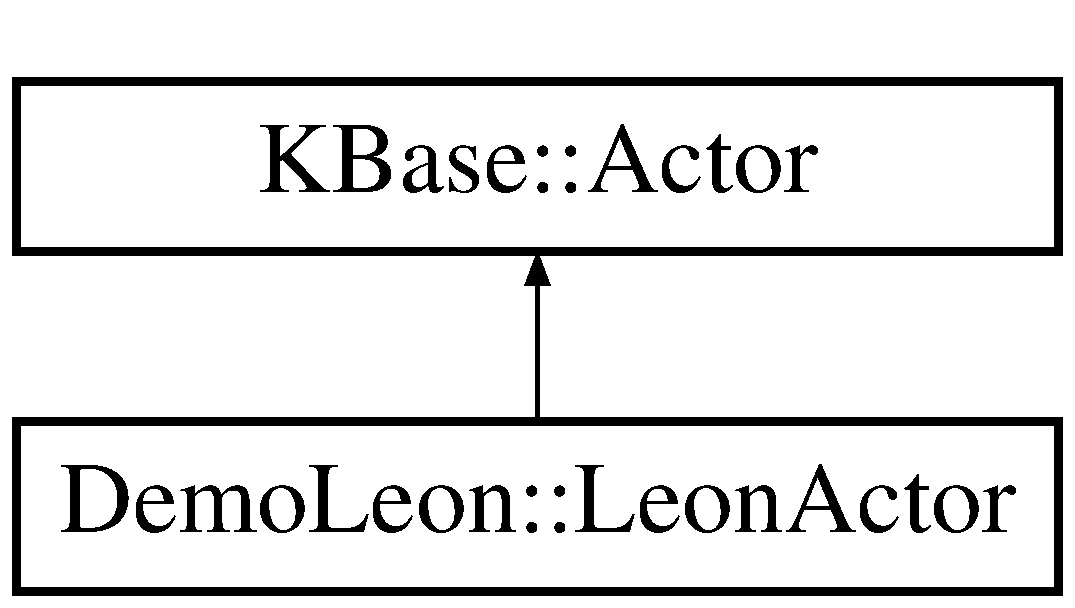
\includegraphics[height=2.000000cm]{class_demo_leon_1_1_leon_actor}
\end{center}
\end{figure}
\subsection*{Public Member Functions}
\begin{DoxyCompactItemize}
\item 
\hypertarget{class_demo_leon_1_1_leon_actor_a0054990f5868d0dea8e12ef966f4fe2c}{{\bfseries Leon\-Actor} (string n, string d, \hyperlink{class_demo_leon_1_1_leon_model}{Leon\-Model} $\ast$em, unsigned int id)}\label{class_demo_leon_1_1_leon_actor_a0054990f5868d0dea8e12ef966f4fe2c}

\item 
\hypertarget{class_demo_leon_1_1_leon_actor_a13dd6848a40e992cb2069bc164dde5cf}{double {\bfseries vote} (unsigned int p1, unsigned int p2, const \hyperlink{class_k_base_1_1_state}{State} $\ast$st) const }\label{class_demo_leon_1_1_leon_actor_a13dd6848a40e992cb2069bc164dde5cf}

\item 
\hypertarget{class_demo_leon_1_1_leon_actor_a341c8116a91ea3afa471e06bbc7626c7}{virtual double {\bfseries vote} (const \hyperlink{class_k_base_1_1_position}{Position} $\ast$ap1, const \hyperlink{class_k_base_1_1_position}{Position} $\ast$ap2) const }\label{class_demo_leon_1_1_leon_actor_a341c8116a91ea3afa471e06bbc7626c7}

\item 
\hypertarget{class_demo_leon_1_1_leon_actor_a4612b58cdb17479cf6011e8c136a1db6}{double {\bfseries pos\-Util} (const \hyperlink{class_k_base_1_1_position}{Position} $\ast$ap1) const }\label{class_demo_leon_1_1_leon_actor_a4612b58cdb17479cf6011e8c136a1db6}

\item 
\hypertarget{class_demo_leon_1_1_leon_actor_a78efd485a0d57e34f16cd05484a6d59c}{void {\bfseries randomize} (\hyperlink{class_k_base_1_1_p_r_n_g}{P\-R\-N\-G} $\ast$rng)}\label{class_demo_leon_1_1_leon_actor_a78efd485a0d57e34f16cd05484a6d59c}

\item 
\hypertarget{class_demo_leon_1_1_leon_actor_a35ce90dd1d5a1f05f1dccd0a5044e2c1}{void {\bfseries set\-Share\-Util\-Scale} (const \hyperlink{class_k_base_1_1_k_matrix}{K\-Matrix} \&runs)}\label{class_demo_leon_1_1_leon_actor_a35ce90dd1d5a1f05f1dccd0a5044e2c1}

\item 
\hypertarget{class_demo_leon_1_1_leon_actor_a272c77831077d3ed3b520eb655e06d84}{double {\bfseries share\-To\-Util} (double gdp\-Share) const }\label{class_demo_leon_1_1_leon_actor_a272c77831077d3ed3b520eb655e06d84}

\end{DoxyCompactItemize}
\subsection*{Public Attributes}
\begin{DoxyCompactItemize}
\item 
\hypertarget{class_demo_leon_1_1_leon_actor_ac1d0763b54385d48548d4a3994b1d6c9}{const \hyperlink{class_demo_leon_1_1_leon_model}{Leon\-Model} $\ast$ {\bfseries e\-Mod} = nullptr}\label{class_demo_leon_1_1_leon_actor_ac1d0763b54385d48548d4a3994b1d6c9}

\item 
\hypertarget{class_demo_leon_1_1_leon_actor_ad1d4a3ecf9f2c2ed114e6e72b69b7aa0}{unsigned int {\bfseries id\-Num} = 0}\label{class_demo_leon_1_1_leon_actor_ad1d4a3ecf9f2c2ed114e6e72b69b7aa0}

\item 
\hypertarget{class_demo_leon_1_1_leon_actor_a7e4e109fc0a7fab6e6d746d8e2eba2b7}{\hyperlink{class_k_base_1_1_k_matrix}{K\-Matrix} {\bfseries v\-Cap} = \hyperlink{class_k_base_1_1_k_matrix}{K\-Matrix}()}\label{class_demo_leon_1_1_leon_actor_a7e4e109fc0a7fab6e6d746d8e2eba2b7}

\item 
\hypertarget{class_demo_leon_1_1_leon_actor_a7a24a56a17b7268a39512c767fc50b9a}{Voting\-Rule {\bfseries vr} = Voting\-Rule\-::\-Proportional}\label{class_demo_leon_1_1_leon_actor_a7a24a56a17b7268a39512c767fc50b9a}

\item 
\hypertarget{class_demo_leon_1_1_leon_actor_a0f213e2a30c168b43b5252cd9f9f6d09}{double {\bfseries min\-S} = 0}\label{class_demo_leon_1_1_leon_actor_a0f213e2a30c168b43b5252cd9f9f6d09}

\item 
\hypertarget{class_demo_leon_1_1_leon_actor_adacbdb6895cae65a8cc7c27f7d30e83e}{double {\bfseries ref\-S} = 0.\-5}\label{class_demo_leon_1_1_leon_actor_adacbdb6895cae65a8cc7c27f7d30e83e}

\item 
\hypertarget{class_demo_leon_1_1_leon_actor_ac4cd6c70e04fc0a13f606386b0027ee2}{double {\bfseries ref\-U} = 0.\-5}\label{class_demo_leon_1_1_leon_actor_ac4cd6c70e04fc0a13f606386b0027ee2}

\item 
\hypertarget{class_demo_leon_1_1_leon_actor_aaa19e5cda5bfc41c29c9d9e05f6995c4}{double {\bfseries max\-S} = 1}\label{class_demo_leon_1_1_leon_actor_aaa19e5cda5bfc41c29c9d9e05f6995c4}

\end{DoxyCompactItemize}
\subsection*{Additional Inherited Members}


The documentation for this class was generated from the following files\-:\begin{DoxyCompactItemize}
\item 
demoleon.\-h\item 
demoleon.\-cpp\end{DoxyCompactItemize}

\hypertarget{class_demo_leon_1_1_leon_model}{\section{Demo\-Leon\-:\-:Leon\-Model Class Reference}
\label{class_demo_leon_1_1_leon_model}\index{Demo\-Leon\-::\-Leon\-Model@{Demo\-Leon\-::\-Leon\-Model}}
}
Inheritance diagram for Demo\-Leon\-:\-:Leon\-Model\-:\begin{figure}[H]
\begin{center}
\leavevmode
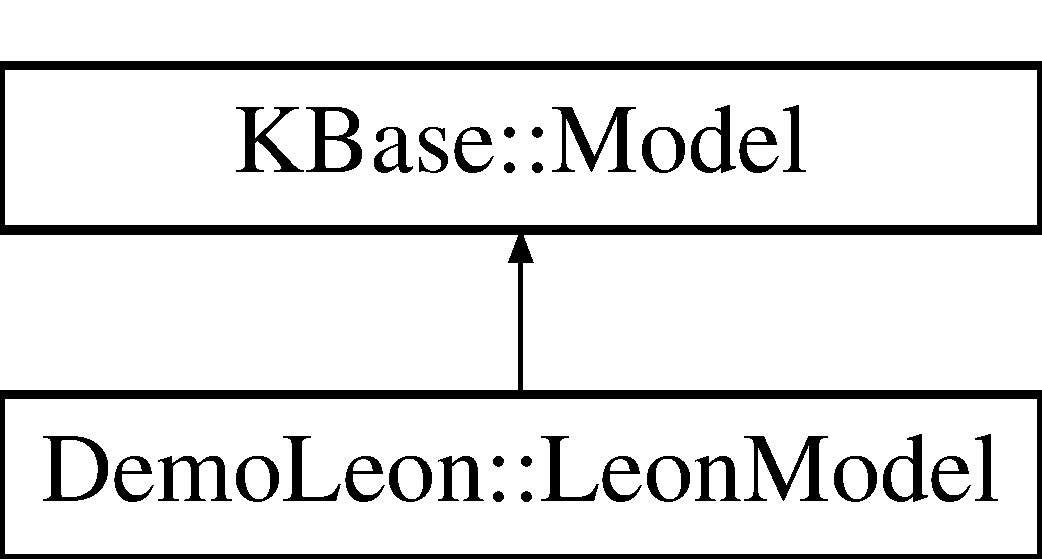
\includegraphics[height=2.000000cm]{class_demo_leon_1_1_leon_model}
\end{center}
\end{figure}
\subsection*{Public Member Functions}
\begin{DoxyCompactItemize}
\item 
\hypertarget{class_demo_leon_1_1_leon_model_ade569b791f144dd09874a6a435d3d454}{{\bfseries Leon\-Model} (\hyperlink{class_k_base_1_1_p_r_n_g}{P\-R\-N\-G} $\ast$r, string d=\char`\"{}\char`\"{})}\label{class_demo_leon_1_1_leon_model_ade569b791f144dd09874a6a435d3d454}

\item 
\hypertarget{class_demo_leon_1_1_leon_model_abe596fe5b6484256d9b6e048ece102b4}{tuple$<$ \hyperlink{class_k_base_1_1_k_matrix}{K\-Matrix}, \hyperlink{class_k_base_1_1_k_matrix}{K\-Matrix}, \\*
\hyperlink{class_k_base_1_1_k_matrix}{K\-Matrix}, \hyperlink{class_k_base_1_1_k_matrix}{K\-Matrix} $>$ {\bfseries make\-Base\-Year} (unsigned int num\-F, unsigned int num\-C\-G, unsigned int num\-S, \hyperlink{class_k_base_1_1_p_r_n_g}{P\-R\-N\-G} $\ast$rng)}\label{class_demo_leon_1_1_leon_model_abe596fe5b6484256d9b6e048ece102b4}

\item 
\hypertarget{class_demo_leon_1_1_leon_model_a4ab04b66ddf45be9856c276b25ab7b14}{void {\bfseries make\-I\-O\-Model} (const \hyperlink{class_k_base_1_1_k_matrix}{K\-Matrix} \&trns, const \hyperlink{class_k_base_1_1_k_matrix}{K\-Matrix} \&rev, const \hyperlink{class_k_base_1_1_k_matrix}{K\-Matrix} \&xprt, const \hyperlink{class_k_base_1_1_k_matrix}{K\-Matrix} \&cons, \hyperlink{class_k_base_1_1_p_r_n_g}{P\-R\-N\-G} $\ast$rng)}\label{class_demo_leon_1_1_leon_model_a4ab04b66ddf45be9856c276b25ab7b14}

\item 
\hypertarget{class_demo_leon_1_1_leon_model_a24be535e2a835331d9e415fceb6b1468}{\hyperlink{class_k_base_1_1_k_matrix}{K\-Matrix} {\bfseries xprt\-Demand} (const \hyperlink{class_k_base_1_1_k_matrix}{K\-Base\-::\-K\-Matrix} \&tau) const }\label{class_demo_leon_1_1_leon_model_a24be535e2a835331d9e415fceb6b1468}

\item 
\hypertarget{class_demo_leon_1_1_leon_model_a86c01fe873755f13556a983c4fe72725}{\hyperlink{class_k_base_1_1_k_matrix}{K\-Matrix} {\bfseries random\-F\-Tax} (\hyperlink{class_k_base_1_1_p_r_n_g}{P\-R\-N\-G} $\ast$rng)}\label{class_demo_leon_1_1_leon_model_a86c01fe873755f13556a983c4fe72725}

\item 
\hypertarget{class_demo_leon_1_1_leon_model_a19b0b95e96472589423854fb825a67f2}{\hyperlink{class_k_base_1_1_k_matrix}{K\-Matrix} {\bfseries make\-F\-Tax} (const \hyperlink{class_k_base_1_1_k_matrix}{K\-Base\-::\-K\-Matrix} \&tax) const }\label{class_demo_leon_1_1_leon_model_a19b0b95e96472589423854fb825a67f2}

\item 
\hypertarget{class_demo_leon_1_1_leon_model_af1676ba2228e7d6a0b96dfeef5349e0c}{double {\bfseries infs\-Degree} (const \hyperlink{class_k_base_1_1_k_matrix}{K\-Matrix} \&tax) const }\label{class_demo_leon_1_1_leon_model_af1676ba2228e7d6a0b96dfeef5349e0c}

\item 
\hypertarget{class_demo_leon_1_1_leon_model_a30ad79a5b30a96f767c4590d19438407}{\hyperlink{class_k_base_1_1_k_matrix}{K\-Matrix} {\bfseries va\-Shares} (const \hyperlink{class_k_base_1_1_k_matrix}{K\-Matrix} \&tax, bool normalize\-Shares\-P) const }\label{class_demo_leon_1_1_leon_model_a30ad79a5b30a96f767c4590d19438407}

\item 
\hypertarget{class_demo_leon_1_1_leon_model_a8ce35fe7efdd8ec3b99f8912d76df45c}{\hyperlink{class_k_base_1_1_k_matrix}{K\-Matrix} {\bfseries monte\-Carlo\-Shares} (unsigned int n\-Runs, \hyperlink{class_k_base_1_1_p_r_n_g}{K\-Base\-::\-P\-R\-N\-G} $\ast$rng)}\label{class_demo_leon_1_1_leon_model_a8ce35fe7efdd8ec3b99f8912d76df45c}

\end{DoxyCompactItemize}
\subsection*{Static Public Member Functions}
\begin{DoxyCompactItemize}
\item 
\hypertarget{class_demo_leon_1_1_leon_model_a61157058f596312006f981d4751e601e}{static double {\bfseries state\-Dist} (const \hyperlink{class_demo_leon_1_1_leon_state}{Leon\-State} $\ast$s1, const \hyperlink{class_demo_leon_1_1_leon_state}{Leon\-State} $\ast$s2)}\label{class_demo_leon_1_1_leon_model_a61157058f596312006f981d4751e601e}

\end{DoxyCompactItemize}
\subsection*{Public Attributes}
\begin{DoxyCompactItemize}
\item 
\hypertarget{class_demo_leon_1_1_leon_model_ac38e9bf87f216341c4224975a36afad8}{double \hyperlink{class_demo_leon_1_1_leon_model_ac38e9bf87f216341c4224975a36afad8}{pos\-Tol} = 1\-E-\/5}\label{class_demo_leon_1_1_leon_model_ac38e9bf87f216341c4224975a36afad8}

\begin{DoxyCompactList}\small\item\em how close together positions must be to be considered equivalent \end{DoxyCompactList}\end{DoxyCompactItemize}
\subsection*{Protected Attributes}
\begin{DoxyCompactItemize}
\item 
\hypertarget{class_demo_leon_1_1_leon_model_ae53e00754cd6c8ad6a05144ff38dca4c}{unsigned int {\bfseries L} = 0}\label{class_demo_leon_1_1_leon_model_ae53e00754cd6c8ad6a05144ff38dca4c}

\item 
\hypertarget{class_demo_leon_1_1_leon_model_ab75a2fe4ee27a617db1e36d596cd9171}{unsigned int {\bfseries M} = 0}\label{class_demo_leon_1_1_leon_model_ab75a2fe4ee27a617db1e36d596cd9171}

\item 
\hypertarget{class_demo_leon_1_1_leon_model_a1890b6bf65909750ca9b6836b6ee538b}{unsigned int {\bfseries N} = 0}\label{class_demo_leon_1_1_leon_model_a1890b6bf65909750ca9b6836b6ee538b}

\item 
\hypertarget{class_demo_leon_1_1_leon_model_af959db8943f55c7849cbab3794b6fef2}{double {\bfseries max\-Sub} = 0.\-5}\label{class_demo_leon_1_1_leon_model_af959db8943f55c7849cbab3794b6fef2}

\item 
\hypertarget{class_demo_leon_1_1_leon_model_a6634250f4c8709ac95da833c2af0eb1f}{double {\bfseries max\-Tax} = 0.\-5}\label{class_demo_leon_1_1_leon_model_a6634250f4c8709ac95da833c2af0eb1f}

\item 
\hypertarget{class_demo_leon_1_1_leon_model_ac1f6f785e7f8f2e56858799f322e4d8c}{\hyperlink{class_k_base_1_1_k_matrix}{K\-Matrix} {\bfseries x0} = \hyperlink{class_k_base_1_1_k_matrix}{K\-Matrix}()}\label{class_demo_leon_1_1_leon_model_ac1f6f785e7f8f2e56858799f322e4d8c}

\item 
\hypertarget{class_demo_leon_1_1_leon_model_a98c15342df03e6959c9c570d54350ace}{\hyperlink{class_k_base_1_1_k_matrix}{K\-Matrix} {\bfseries eps} = \hyperlink{class_k_base_1_1_k_matrix}{K\-Matrix}()}\label{class_demo_leon_1_1_leon_model_a98c15342df03e6959c9c570d54350ace}

\item 
\hypertarget{class_demo_leon_1_1_leon_model_ac4d3ea6c799789e2821c4cb55b750c31}{\hyperlink{class_k_base_1_1_k_matrix}{K\-Matrix} {\bfseries a\-L} = \hyperlink{class_k_base_1_1_k_matrix}{K\-Matrix}()}\label{class_demo_leon_1_1_leon_model_ac4d3ea6c799789e2821c4cb55b750c31}

\item 
\hypertarget{class_demo_leon_1_1_leon_model_a079da964cfd291c6379a3f8f3b4eb007}{\hyperlink{class_k_base_1_1_k_matrix}{K\-Matrix} {\bfseries b\-L} = \hyperlink{class_k_base_1_1_k_matrix}{K\-Matrix}()}\label{class_demo_leon_1_1_leon_model_a079da964cfd291c6379a3f8f3b4eb007}

\item 
\hypertarget{class_demo_leon_1_1_leon_model_a65f640d25245c6f6b70c63bf5770a95c}{\hyperlink{class_k_base_1_1_k_matrix}{K\-Matrix} {\bfseries rho} = \hyperlink{class_k_base_1_1_k_matrix}{K\-Matrix}()}\label{class_demo_leon_1_1_leon_model_a65f640d25245c6f6b70c63bf5770a95c}

\item 
\hypertarget{class_demo_leon_1_1_leon_model_acc79412a1612323750d7f09064f46db2}{\hyperlink{class_k_base_1_1_k_matrix}{K\-Matrix} {\bfseries vas} = \hyperlink{class_k_base_1_1_k_matrix}{K\-Matrix}()}\label{class_demo_leon_1_1_leon_model_acc79412a1612323750d7f09064f46db2}

\end{DoxyCompactItemize}
\subsection*{Friends}
\begin{DoxyCompactItemize}
\item 
\hypertarget{class_demo_leon_1_1_leon_model_a5cf4577c974c9fdb3f8af300f80e7c8e}{class {\bfseries Leon\-Actor}}\label{class_demo_leon_1_1_leon_model_a5cf4577c974c9fdb3f8af300f80e7c8e}

\end{DoxyCompactItemize}
\subsection*{Additional Inherited Members}


The documentation for this class was generated from the following files\-:\begin{DoxyCompactItemize}
\item 
demoleon.\-h\item 
demoleon.\-cpp\end{DoxyCompactItemize}

\hypertarget{class_demo_leon_1_1_leon_state}{\section{Demo\-Leon\-:\-:Leon\-State Class Reference}
\label{class_demo_leon_1_1_leon_state}\index{Demo\-Leon\-::\-Leon\-State@{Demo\-Leon\-::\-Leon\-State}}
}
Inheritance diagram for Demo\-Leon\-:\-:Leon\-State\-:\begin{figure}[H]
\begin{center}
\leavevmode
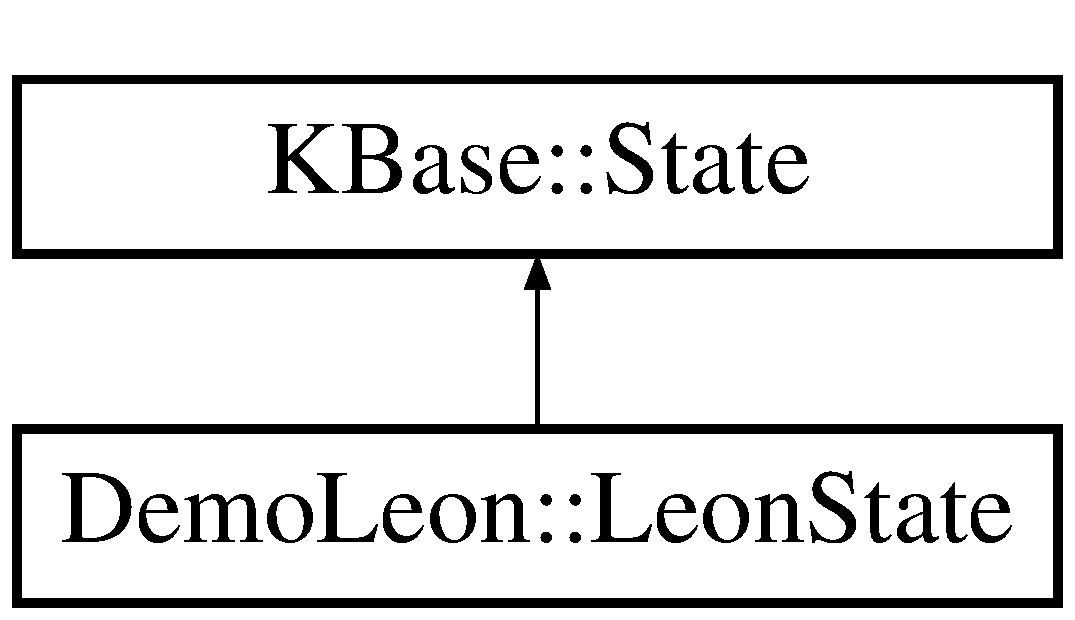
\includegraphics[height=2.000000cm]{class_demo_leon_1_1_leon_state}
\end{center}
\end{figure}
\subsection*{Public Member Functions}
\begin{DoxyCompactItemize}
\item 
\hypertarget{class_demo_leon_1_1_leon_state_a0e5f459528f4801a4560134111f7686f}{{\bfseries Leon\-State} (\hyperlink{class_demo_leon_1_1_leon_model}{Leon\-Model} $\ast$em)}\label{class_demo_leon_1_1_leon_state_a0e5f459528f4801a4560134111f7686f}

\item 
\hypertarget{class_demo_leon_1_1_leon_state_ab2a009cd1b0b6413d695e819346c8e5e}{virtual tuple$<$ \hyperlink{class_k_base_1_1_k_matrix}{K\-Matrix}, V\-U\-I $>$ {\bfseries p\-Dist} (int persp) const }\label{class_demo_leon_1_1_leon_state_ab2a009cd1b0b6413d695e819346c8e5e}

\item 
\hypertarget{class_demo_leon_1_1_leon_state_a96d90fb82535febd36bbfdf8be8c7286}{\hyperlink{class_demo_leon_1_1_leon_state}{Leon\-State} $\ast$ {\bfseries step\-S\-U\-S\-N} ()}\label{class_demo_leon_1_1_leon_state_a96d90fb82535febd36bbfdf8be8c7286}

\end{DoxyCompactItemize}
\subsection*{Public Attributes}
\begin{DoxyCompactItemize}
\item 
\hypertarget{class_demo_leon_1_1_leon_state_adbf4164390a52544c94c9b90460910b7}{const \hyperlink{class_demo_leon_1_1_leon_model}{Leon\-Model} $\ast$ {\bfseries e\-Mod} = nullptr}\label{class_demo_leon_1_1_leon_state_adbf4164390a52544c94c9b90460910b7}

\end{DoxyCompactItemize}
\subsection*{Protected Member Functions}
\begin{DoxyCompactItemize}
\item 
\hypertarget{class_demo_leon_1_1_leon_state_a44c36c0ef0dd1371dc005137983a8ada}{\hyperlink{class_demo_leon_1_1_leon_state}{Leon\-State} $\ast$ {\bfseries do\-S\-U\-S\-N} (Reporting\-Level rl) const }\label{class_demo_leon_1_1_leon_state_a44c36c0ef0dd1371dc005137983a8ada}

\item 
virtual bool \hyperlink{class_demo_leon_1_1_leon_state_ae8f61a8c082dd80a8270019e4cf3633f}{equiv\-Ndx} (unsigned int i, unsigned int j) const 
\item 
\hypertarget{class_demo_leon_1_1_leon_state_ad60c15038d56b10b57f3a7ae6b4684c8}{void {\bfseries set\-All\-A\-Util} (Reporting\-Level rl)}\label{class_demo_leon_1_1_leon_state_ad60c15038d56b10b57f3a7ae6b4684c8}

\end{DoxyCompactItemize}
\subsection*{Additional Inherited Members}


\subsection{Member Function Documentation}
\hypertarget{class_demo_leon_1_1_leon_state_ae8f61a8c082dd80a8270019e4cf3633f}{\index{Demo\-Leon\-::\-Leon\-State@{Demo\-Leon\-::\-Leon\-State}!equiv\-Ndx@{equiv\-Ndx}}
\index{equiv\-Ndx@{equiv\-Ndx}!DemoLeon::LeonState@{Demo\-Leon\-::\-Leon\-State}}
\subsubsection[{equiv\-Ndx}]{\setlength{\rightskip}{0pt plus 5cm}bool Demo\-Leon\-::\-Leon\-State\-::equiv\-Ndx (
\begin{DoxyParamCaption}
\item[{unsigned int}]{i, }
\item[{unsigned int}]{j}
\end{DoxyParamCaption}
) const\hspace{0.3cm}{\ttfamily [protected]}, {\ttfamily [virtual]}}}\label{class_demo_leon_1_1_leon_state_ae8f61a8c082dd80a8270019e4cf3633f}
Compare two actual positions in the current state 

Implements \hyperlink{class_k_base_1_1_state}{K\-Base\-::\-State}.



The documentation for this class was generated from the following files\-:\begin{DoxyCompactItemize}
\item 
demoleon.\-h\item 
demoleon.\-cpp\end{DoxyCompactItemize}

\hypertarget{class_k_base_1_1_model}{\section{K\-Base\-:\-:Model Class Reference}
\label{class_k_base_1_1_model}\index{K\-Base\-::\-Model@{K\-Base\-::\-Model}}
}
Inheritance diagram for K\-Base\-:\-:Model\-:\begin{figure}[H]
\begin{center}
\leavevmode
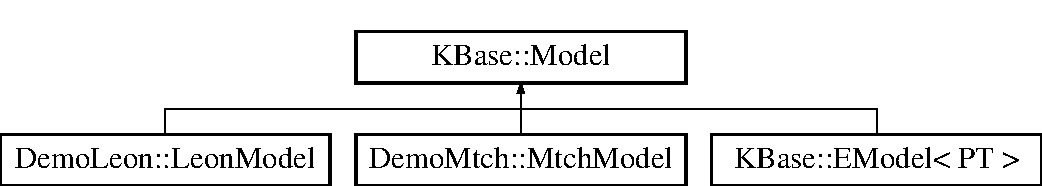
\includegraphics[height=2.000000cm]{class_k_base_1_1_model}
\end{center}
\end{figure}
\subsection*{Public Member Functions}
\begin{DoxyCompactItemize}
\item 
\hypertarget{class_k_base_1_1_model_a721ae81e6022dfe3f9850d5acbdd64ac}{{\bfseries Model} (\hyperlink{class_k_base_1_1_p_r_n_g}{P\-R\-N\-G} $\ast$r, string d)}\label{class_k_base_1_1_model_a721ae81e6022dfe3f9850d5acbdd64ac}

\item 
\hypertarget{class_k_base_1_1_model_a92e31c17c2d2d25ecbb5e97d4b2dc2db}{void {\bfseries run} ()}\label{class_k_base_1_1_model_a92e31c17c2d2d25ecbb5e97d4b2dc2db}

\item 
\hypertarget{class_k_base_1_1_model_ac33c6195259a8ec6ad2e048c217df06c}{virtual unsigned int {\bfseries add\-Actor} (\hyperlink{class_k_base_1_1_actor}{Actor} $\ast$a)}\label{class_k_base_1_1_model_ac33c6195259a8ec6ad2e048c217df06c}

\item 
\hypertarget{class_k_base_1_1_model_a6b642668bf98d62805388c00132834fd}{int {\bfseries actr\-Ndx} (const \hyperlink{class_k_base_1_1_actor}{Actor} $\ast$a) const }\label{class_k_base_1_1_model_a6b642668bf98d62805388c00132834fd}

\item 
\hypertarget{class_k_base_1_1_model_a8743cd5a9b81d98eccada6c75890f0b5}{int {\bfseries add\-State} (\hyperlink{class_k_base_1_1_state}{State} $\ast$s)}\label{class_k_base_1_1_model_a8743cd5a9b81d98eccada6c75890f0b5}

\item 
\hypertarget{class_k_base_1_1_model_a01c7a648c69fbc0a99fff05b678417f9}{void {\bfseries sql\-A\-Util} (unsigned int t)}\label{class_k_base_1_1_model_a01c7a648c69fbc0a99fff05b678417f9}

\end{DoxyCompactItemize}
\subsection*{Static Public Member Functions}
\begin{DoxyCompactItemize}
\item 
\hypertarget{class_k_base_1_1_model_a9bcd9a07fc288091d13d662e171390d3}{static double {\bfseries n\-Prod} (double x, double y)}\label{class_k_base_1_1_model_a9bcd9a07fc288091d13d662e171390d3}

\item 
\hypertarget{class_k_base_1_1_model_a7816a87892ced9fa979d76954da13b8c}{static double {\bfseries vote} (Voting\-Rule vr, double wi, double uij, double uik)}\label{class_k_base_1_1_model_a7816a87892ced9fa979d76954da13b8c}

\item 
\hypertarget{class_k_base_1_1_model_a988856a6236fa8312c04a03168d57f50}{static \hyperlink{class_k_base_1_1_k_matrix}{K\-Matrix} {\bfseries coalitions} (function$<$ double(unsigned int ak, unsigned int pi, unsigned int pj)$>$ vfn, unsigned int num\-Act, unsigned int num\-Opt)}\label{class_k_base_1_1_model_a988856a6236fa8312c04a03168d57f50}

\item 
\hypertarget{class_k_base_1_1_model_a440319f89298fba52901e435a3153a57}{static \hyperlink{class_k_base_1_1_k_matrix}{K\-Matrix} {\bfseries v\-Prob} (V\-P\-Model vpm, const \hyperlink{class_k_base_1_1_k_matrix}{K\-Matrix} \&c)}\label{class_k_base_1_1_model_a440319f89298fba52901e435a3153a57}

\item 
\hypertarget{class_k_base_1_1_model_a3f34db18c88892cd4db03e3c019e78c5}{static \hyperlink{class_k_base_1_1_k_matrix}{K\-Matrix} {\bfseries v\-Prob} (Voting\-Rule vr, V\-P\-Model vpm, const \hyperlink{class_k_base_1_1_k_matrix}{K\-Matrix} \&w, const \hyperlink{class_k_base_1_1_k_matrix}{K\-Matrix} \&u)}\label{class_k_base_1_1_model_a3f34db18c88892cd4db03e3c019e78c5}

\item 
\hypertarget{class_k_base_1_1_model_a352b8be7b7bb6814e990dcedc08df8da}{static \hyperlink{class_k_base_1_1_k_matrix}{K\-Matrix} {\bfseries prob\-C\-E} (P\-C\-E\-Model pcm, const \hyperlink{class_k_base_1_1_k_matrix}{K\-Matrix} \&pv)}\label{class_k_base_1_1_model_a352b8be7b7bb6814e990dcedc08df8da}

\item 
\hypertarget{class_k_base_1_1_model_aa2a04e5142714ee3194fd8656cdffbc4}{static \hyperlink{class_k_base_1_1_k_matrix}{K\-Matrix} {\bfseries scalar\-P\-C\-E} (unsigned int num\-Act, unsigned int num\-Opt, const \hyperlink{class_k_base_1_1_k_matrix}{K\-Matrix} \&w, const \hyperlink{class_k_base_1_1_k_matrix}{K\-Matrix} \&u, Voting\-Rule vr, V\-P\-Model vpm, Reporting\-Level rl)}\label{class_k_base_1_1_model_aa2a04e5142714ee3194fd8656cdffbc4}

\item 
\hypertarget{class_k_base_1_1_model_a1d963fdaaf8e9f40cdc43ed025f0b5c1}{static void {\bfseries demo\-S\-Q\-Lite} ()}\label{class_k_base_1_1_model_a1d963fdaaf8e9f40cdc43ed025f0b5c1}

\item 
\hypertarget{class_k_base_1_1_model_a1ea7a9fdd03329f6bf0234bb4d43edb6}{static \hyperlink{class_k_base_1_1_k_matrix}{K\-Matrix} {\bfseries big\-Rfrom\-Prob} (const \hyperlink{class_k_base_1_1_k_matrix}{K\-Matrix} \&p, Big\-R\-Range rr)}\label{class_k_base_1_1_model_a1ea7a9fdd03329f6bf0234bb4d43edb6}

\item 
\hypertarget{class_k_base_1_1_model_aa13a028a9eb4cad23c934f50f9f70fe4}{static double {\bfseries est\-N\-R\-A} (double rh, double ri, Big\-R\-Adjust ra)}\label{class_k_base_1_1_model_aa13a028a9eb4cad23c934f50f9f70fe4}

\end{DoxyCompactItemize}
\subsection*{Public Attributes}
\begin{DoxyCompactItemize}
\item 
\hypertarget{class_k_base_1_1_model_a0605824758cb36c2e9d4ca15407296a5}{function$<$ bool(unsigned int \\*
iter, const \hyperlink{class_k_base_1_1_state}{State} $\ast$s)$>$ {\bfseries stop} = nullptr}\label{class_k_base_1_1_model_a0605824758cb36c2e9d4ca15407296a5}

\item 
\hypertarget{class_k_base_1_1_model_a4fb640f320147e67c05c0de5bd33922e}{vector$<$ \hyperlink{class_k_base_1_1_actor}{Actor} $\ast$ $>$ {\bfseries actrs} = \{\}}\label{class_k_base_1_1_model_a4fb640f320147e67c05c0de5bd33922e}

\item 
\hypertarget{class_k_base_1_1_model_a54dbb244fe386a7d9c4f29f1b14ba07a}{unsigned int {\bfseries num\-Act} = 0}\label{class_k_base_1_1_model_a54dbb244fe386a7d9c4f29f1b14ba07a}

\item 
\hypertarget{class_k_base_1_1_model_a863472bdfea740b5978f961be09ee6c8}{\hyperlink{class_k_base_1_1_p_r_n_g}{P\-R\-N\-G} $\ast$ {\bfseries rng} = nullptr}\label{class_k_base_1_1_model_a863472bdfea740b5978f961be09ee6c8}

\item 
\hypertarget{class_k_base_1_1_model_adc4ad033725b177ba804e4aeab3b6a98}{vector$<$ \hyperlink{class_k_base_1_1_state}{State} $\ast$ $>$ {\bfseries history} = \{\}}\label{class_k_base_1_1_model_adc4ad033725b177ba804e4aeab3b6a98}

\end{DoxyCompactItemize}
\subsection*{Static Protected Member Functions}
\begin{DoxyCompactItemize}
\item 
\hypertarget{class_k_base_1_1_model_a4f9616242374d83dec4fadb954a6af67}{static string {\bfseries create\-Table\-S\-Q\-L} (unsigned int tn)}\label{class_k_base_1_1_model_a4f9616242374d83dec4fadb954a6af67}

\item 
\hypertarget{class_k_base_1_1_model_a94bb7e9c4b5cd9c5de1cab7abec12e70}{static tuple$<$ double, double $>$ {\bfseries v\-Prob} (V\-P\-Model vpm, const double s1, const double s2)}\label{class_k_base_1_1_model_a94bb7e9c4b5cd9c5de1cab7abec12e70}

\item 
\hypertarget{class_k_base_1_1_model_a7d265a8cd6b8c42fa933626ead61e70d}{static \hyperlink{class_k_base_1_1_k_matrix}{K\-Matrix} {\bfseries markov\-P\-C\-E} (const \hyperlink{class_k_base_1_1_k_matrix}{K\-Matrix} \&pv)}\label{class_k_base_1_1_model_a7d265a8cd6b8c42fa933626ead61e70d}

\item 
\hypertarget{class_k_base_1_1_model_a8e920c4a2ffc517e171cc39d60feb5f1}{static \hyperlink{class_k_base_1_1_k_matrix}{K\-Matrix} {\bfseries cond\-P\-C\-E} (const \hyperlink{class_k_base_1_1_k_matrix}{K\-Matrix} \&pv)}\label{class_k_base_1_1_model_a8e920c4a2ffc517e171cc39d60feb5f1}

\end{DoxyCompactItemize}
\subsection*{Protected Attributes}
\begin{DoxyCompactItemize}
\item 
\hypertarget{class_k_base_1_1_model_a41d171a405093172d905ab3351be3a38}{sqlite3 $\ast$ {\bfseries smp\-D\-B} = nullptr}\label{class_k_base_1_1_model_a41d171a405093172d905ab3351be3a38}

\item 
\hypertarget{class_k_base_1_1_model_a73e69311b9afd8c8b0c4c43bfd07d994}{string {\bfseries scen\-Name} = \char`\"{}Scen\char`\"{}}\label{class_k_base_1_1_model_a73e69311b9afd8c8b0c4c43bfd07d994}

\end{DoxyCompactItemize}


The documentation for this class was generated from the following files\-:\begin{DoxyCompactItemize}
\item 
kmodel.\-h\item 
kmodel.\-cpp\item 
kmodelsql.\-cpp\end{DoxyCompactItemize}

\hypertarget{class_demo_mtch_1_1_mtch_actor}{\section{Demo\-Mtch\-:\-:Mtch\-Actor Class Reference}
\label{class_demo_mtch_1_1_mtch_actor}\index{Demo\-Mtch\-::\-Mtch\-Actor@{Demo\-Mtch\-::\-Mtch\-Actor}}
}
Inheritance diagram for Demo\-Mtch\-:\-:Mtch\-Actor\-:\begin{figure}[H]
\begin{center}
\leavevmode
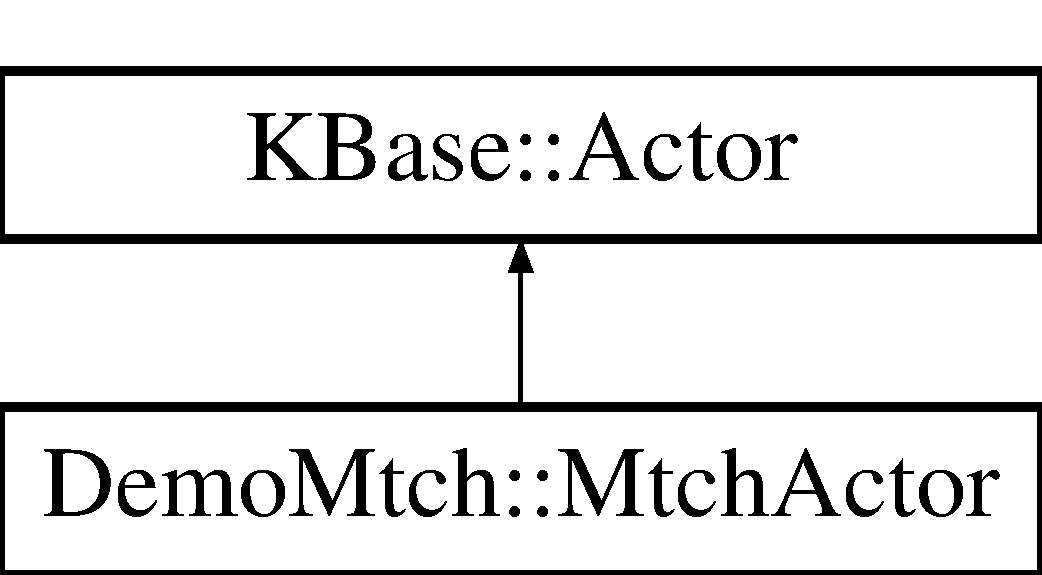
\includegraphics[height=2.000000cm]{class_demo_mtch_1_1_mtch_actor}
\end{center}
\end{figure}
\subsection*{Public Types}
\begin{DoxyCompactItemize}
\item 
enum {\bfseries Prop\-Model} \{ {\bfseries Exp\-Util}, 
{\bfseries Probability}, 
{\bfseries Agree\-Util}
 \}
\end{DoxyCompactItemize}
\subsection*{Public Member Functions}
\begin{DoxyCompactItemize}
\item 
\hypertarget{class_demo_mtch_1_1_mtch_actor_ab88051b8646350e53e422cc6803db997}{{\bfseries Mtch\-Actor} (string n, string d)}\label{class_demo_mtch_1_1_mtch_actor_ab88051b8646350e53e422cc6803db997}

\item 
\hypertarget{class_demo_mtch_1_1_mtch_actor_a14bfaf0d6e9a5d767f46855ef206738a}{double {\bfseries vote} (unsigned int p1, unsigned int p2, const \hyperlink{class_k_base_1_1_state}{State} $\ast$st) const }\label{class_demo_mtch_1_1_mtch_actor_a14bfaf0d6e9a5d767f46855ef206738a}

\item 
\hypertarget{class_demo_mtch_1_1_mtch_actor_aa1414cdffb187a2d14ae3b30ce5686d8}{virtual double {\bfseries vote} (const \hyperlink{class_k_base_1_1_position}{Position} $\ast$ap1, const \hyperlink{class_k_base_1_1_position}{Position} $\ast$ap2) const }\label{class_demo_mtch_1_1_mtch_actor_aa1414cdffb187a2d14ae3b30ce5686d8}

\item 
\hypertarget{class_demo_mtch_1_1_mtch_actor_a124d78dfcb5499dc900206db5dd80753}{double {\bfseries pos\-Util} (const \hyperlink{class_k_base_1_1_position}{Position} $\ast$ap1) const }\label{class_demo_mtch_1_1_mtch_actor_a124d78dfcb5499dc900206db5dd80753}

\item 
\hypertarget{class_demo_mtch_1_1_mtch_actor_adfa057a20bf1245dadc78ba2b1c034c5}{void {\bfseries randomize} (\hyperlink{class_k_base_1_1_p_r_n_g}{P\-R\-N\-G} $\ast$rng, double min\-Cap, double max\-Cap, unsigned int id, unsigned int num\-I)}\label{class_demo_mtch_1_1_mtch_actor_adfa057a20bf1245dadc78ba2b1c034c5}

\item 
\hypertarget{class_demo_mtch_1_1_mtch_actor_a2a6a0273d00b2ccc996ccf0c959d4742}{tuple$<$ double, \hyperlink{class_k_base_1_1_mtch_pstn}{Mtch\-Pstn} $>$ {\bfseries max\-Prob\-E\-U\-Pstn} (Prop\-Model pm, const \hyperlink{class_demo_mtch_1_1_mtch_state}{Mtch\-State} $\ast$mst) const }\label{class_demo_mtch_1_1_mtch_actor_a2a6a0273d00b2ccc996ccf0c959d4742}

\end{DoxyCompactItemize}
\subsection*{Static Public Member Functions}
\begin{DoxyCompactItemize}
\item 
\hypertarget{class_demo_mtch_1_1_mtch_actor_afdccb60bbf9b804a6ffe6ab07d666752}{static \hyperlink{class_k_base_1_1_mtch_pstn}{Mtch\-Pstn} $\ast$ {\bfseries r\-Pos} (unsigned int num\-I, unsigned int num\-A, \hyperlink{class_k_base_1_1_p_r_n_g}{P\-R\-N\-G} $\ast$rng)}\label{class_demo_mtch_1_1_mtch_actor_afdccb60bbf9b804a6ffe6ab07d666752}

\item 
\hypertarget{class_demo_mtch_1_1_mtch_actor_af613e5a133e782ae62cf3b5b26c1fc45}{static \hyperlink{class_demo_mtch_1_1_mtch_actor}{Mtch\-Actor} $\ast$ {\bfseries r\-Act} (unsigned int num\-I, double min\-Cap, double max\-Cap, \hyperlink{class_k_base_1_1_p_r_n_g}{P\-R\-N\-G} $\ast$rng, unsigned int i)}\label{class_demo_mtch_1_1_mtch_actor_af613e5a133e782ae62cf3b5b26c1fc45}

\end{DoxyCompactItemize}
\subsection*{Public Attributes}
\begin{DoxyCompactItemize}
\item 
\hypertarget{class_demo_mtch_1_1_mtch_actor_a6620ce7762057a59fc3a1a98218a6fcf}{unsigned int {\bfseries id\-Num} = 0}\label{class_demo_mtch_1_1_mtch_actor_a6620ce7762057a59fc3a1a98218a6fcf}

\item 
\hypertarget{class_demo_mtch_1_1_mtch_actor_a98229798fc76627c2bf2a630a9ae45d7}{Voting\-Rule {\bfseries vr} = Voting\-Rule\-::\-Proportional}\label{class_demo_mtch_1_1_mtch_actor_a98229798fc76627c2bf2a630a9ae45d7}

\item 
\hypertarget{class_demo_mtch_1_1_mtch_actor_a1adca2569c4a1ecfa133addad09937e7}{Prop\-Model {\bfseries p\-Mod} = Prop\-Model\-::\-Exp\-Util}\label{class_demo_mtch_1_1_mtch_actor_a1adca2569c4a1ecfa133addad09937e7}

\item 
\hypertarget{class_demo_mtch_1_1_mtch_actor_aa61012a0056831027648d2a0e03f04f9}{double {\bfseries s\-Cap} = 0}\label{class_demo_mtch_1_1_mtch_actor_aa61012a0056831027648d2a0e03f04f9}

\item 
\hypertarget{class_demo_mtch_1_1_mtch_actor_a8949d6d327fc75b24f53e010bc24537d}{vector$<$ double $>$ {\bfseries vals} = \{\}}\label{class_demo_mtch_1_1_mtch_actor_a8949d6d327fc75b24f53e010bc24537d}

\end{DoxyCompactItemize}


The documentation for this class was generated from the following files\-:\begin{DoxyCompactItemize}
\item 
demomtch.\-h\item 
demomtch.\-cpp\end{DoxyCompactItemize}

\hypertarget{class_k_base_1_1_mtch_gene}{\section{K\-Base\-:\-:Mtch\-Gene Class Reference}
\label{class_k_base_1_1_mtch_gene}\index{K\-Base\-::\-Mtch\-Gene@{K\-Base\-::\-Mtch\-Gene}}
}
Inheritance diagram for K\-Base\-:\-:Mtch\-Gene\-:\begin{figure}[H]
\begin{center}
\leavevmode
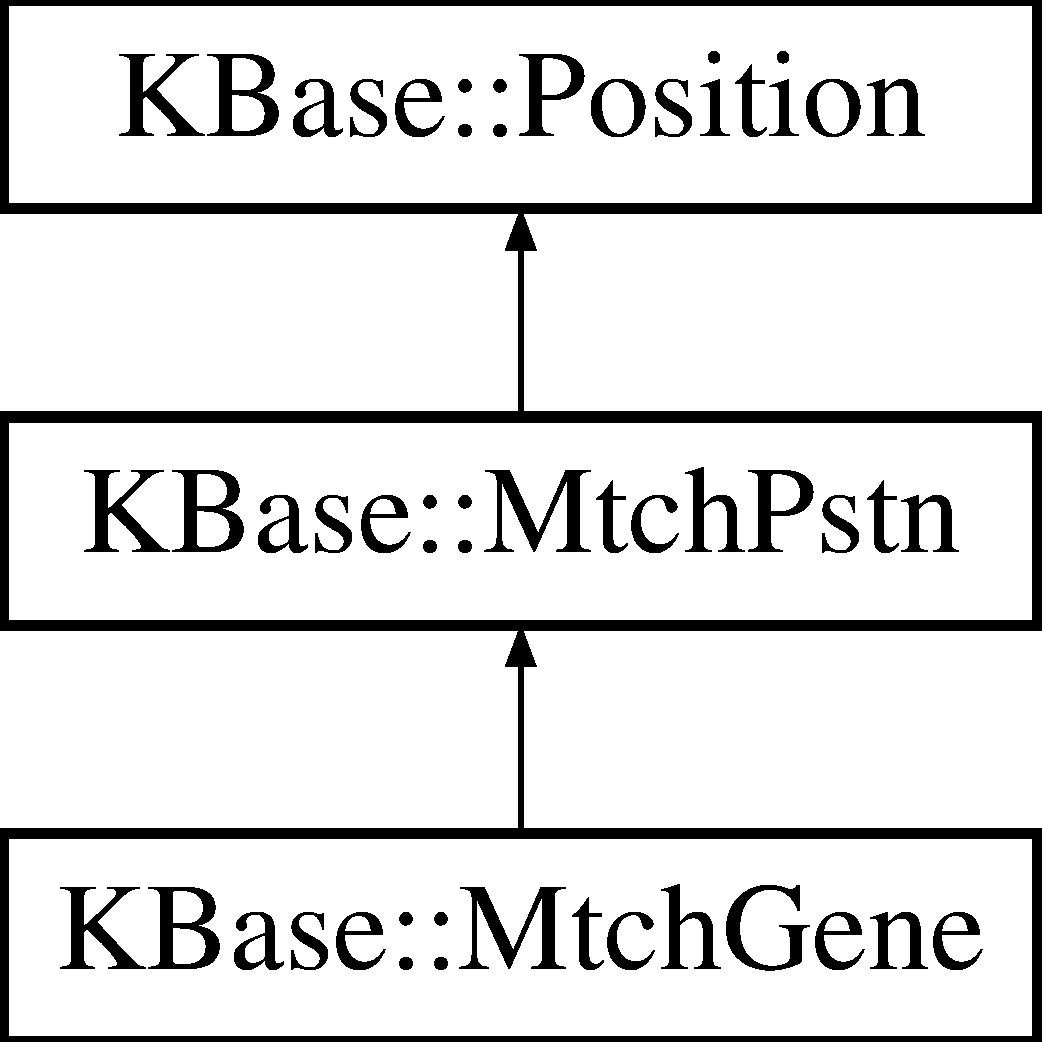
\includegraphics[height=3.000000cm]{class_k_base_1_1_mtch_gene}
\end{center}
\end{figure}
\subsection*{Public Member Functions}
\begin{DoxyCompactItemize}
\item 
\hypertarget{class_k_base_1_1_mtch_gene_a8386c386632b4e6dd8a99f3f126f0899}{void {\bfseries randomize} (\hyperlink{class_k_base_1_1_p_r_n_g}{P\-R\-N\-G} $\ast$rng)}\label{class_k_base_1_1_mtch_gene_a8386c386632b4e6dd8a99f3f126f0899}

\item 
\hypertarget{class_k_base_1_1_mtch_gene_a489185a8e050f4d697fda5bcbb14d304}{\hyperlink{class_k_base_1_1_mtch_gene}{Mtch\-Gene} $\ast$ {\bfseries mutate} (\hyperlink{class_k_base_1_1_p_r_n_g}{P\-R\-N\-G} $\ast$rng) const }\label{class_k_base_1_1_mtch_gene_a489185a8e050f4d697fda5bcbb14d304}

\item 
\hypertarget{class_k_base_1_1_mtch_gene_a7d33dcc982a4a74a760cb086309fa141}{tuple$<$ \hyperlink{class_k_base_1_1_mtch_gene}{Mtch\-Gene} $\ast$, \hyperlink{class_k_base_1_1_mtch_gene}{Mtch\-Gene} $\ast$ $>$ {\bfseries cross} (const \hyperlink{class_k_base_1_1_mtch_gene}{Mtch\-Gene} $\ast$g2, \hyperlink{class_k_base_1_1_p_r_n_g}{P\-R\-N\-G} $\ast$rng) const }\label{class_k_base_1_1_mtch_gene_a7d33dcc982a4a74a760cb086309fa141}

\item 
\hypertarget{class_k_base_1_1_mtch_gene_a686f60ab70b9bb2cc523a3fd191ee611}{bool {\bfseries equiv} (const \hyperlink{class_k_base_1_1_mtch_gene}{Mtch\-Gene} $\ast$g2) const }\label{class_k_base_1_1_mtch_gene_a686f60ab70b9bb2cc523a3fd191ee611}

\item 
\hypertarget{class_k_base_1_1_mtch_gene_a62261a1e6a71765badd513976c8679e7}{void {\bfseries set\-State} (vector$<$ \hyperlink{class_k_base_1_1_actor}{Actor} $\ast$ $>$ as, vector$<$ \hyperlink{class_k_base_1_1_mtch_pstn}{Mtch\-Pstn} $\ast$ $>$ ps)}\label{class_k_base_1_1_mtch_gene_a62261a1e6a71765badd513976c8679e7}

\end{DoxyCompactItemize}
\subsection*{Protected Member Functions}
\begin{DoxyCompactItemize}
\item 
\hypertarget{class_k_base_1_1_mtch_gene_a1b8e3837418c427591c9acbc32f04a17}{virtual void {\bfseries print} (ostream \&os) const }\label{class_k_base_1_1_mtch_gene_a1b8e3837418c427591c9acbc32f04a17}

\item 
\hypertarget{class_k_base_1_1_mtch_gene_a7f8ae683f1e19a013ec4da4baaefa6c9}{void {\bfseries copy\-Self} (\hyperlink{class_k_base_1_1_mtch_gene}{Mtch\-Gene} $\ast$) const }\label{class_k_base_1_1_mtch_gene_a7f8ae683f1e19a013ec4da4baaefa6c9}

\end{DoxyCompactItemize}
\subsection*{Protected Attributes}
\begin{DoxyCompactItemize}
\item 
\hypertarget{class_k_base_1_1_mtch_gene_aede2ca17f3b313d8e291bf8a9c0d9866}{vector$<$ \hyperlink{class_k_base_1_1_actor}{Actor} $\ast$ $>$ {\bfseries actrs} = \{\}}\label{class_k_base_1_1_mtch_gene_aede2ca17f3b313d8e291bf8a9c0d9866}

\item 
\hypertarget{class_k_base_1_1_mtch_gene_a9f4788155664c1ba7b34064ce14a255e}{vector$<$ \hyperlink{class_k_base_1_1_mtch_pstn}{Mtch\-Pstn} $\ast$ $>$ {\bfseries pstns} = \{\}}\label{class_k_base_1_1_mtch_gene_a9f4788155664c1ba7b34064ce14a255e}

\end{DoxyCompactItemize}
\subsection*{Additional Inherited Members}


The documentation for this class was generated from the following files\-:\begin{DoxyCompactItemize}
\item 
kmodel.\-h\item 
kposition.\-cpp\end{DoxyCompactItemize}

\hypertarget{class_demo_mtch_1_1_mtch_model}{\section{Demo\-Mtch\-:\-:Mtch\-Model Class Reference}
\label{class_demo_mtch_1_1_mtch_model}\index{Demo\-Mtch\-::\-Mtch\-Model@{Demo\-Mtch\-::\-Mtch\-Model}}
}
Inheritance diagram for Demo\-Mtch\-:\-:Mtch\-Model\-:\begin{figure}[H]
\begin{center}
\leavevmode
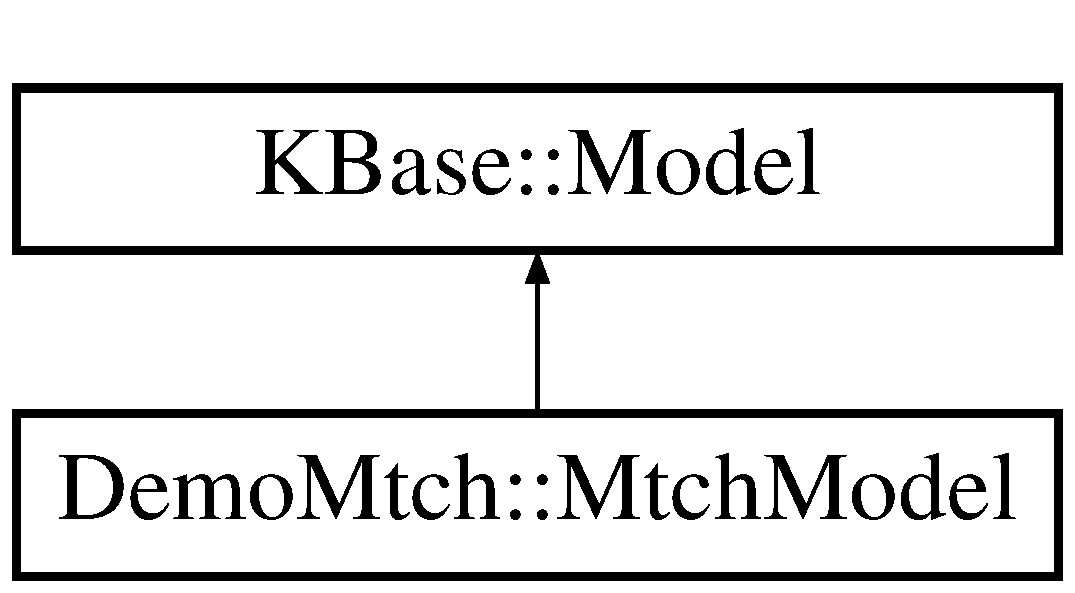
\includegraphics[height=2.000000cm]{class_demo_mtch_1_1_mtch_model}
\end{center}
\end{figure}
\subsection*{Public Member Functions}
\begin{DoxyCompactItemize}
\item 
\hypertarget{class_demo_mtch_1_1_mtch_model_ab3b0b8b87f85ef9043df8283d805b56e}{{\bfseries Mtch\-Model} (\hyperlink{class_k_base_1_1_p_r_n_g}{P\-R\-N\-G} $\ast$rng, string d=\char`\"{}\char`\"{})}\label{class_demo_mtch_1_1_mtch_model_ab3b0b8b87f85ef9043df8283d805b56e}

\end{DoxyCompactItemize}
\subsection*{Static Public Member Functions}
\begin{DoxyCompactItemize}
\item 
\hypertarget{class_demo_mtch_1_1_mtch_model_a23dd4a323f33e41049389e7b13a72f8c}{static \hyperlink{class_demo_mtch_1_1_mtch_model}{Mtch\-Model} $\ast$ {\bfseries random\-M\-S} (unsigned int num\-A, unsigned int num\-I, Voting\-Rule vr, Mtch\-Actor\-::\-Prop\-Model p\-Mod, \hyperlink{class_k_base_1_1_p_r_n_g}{P\-R\-N\-G} $\ast$rng)}\label{class_demo_mtch_1_1_mtch_model_a23dd4a323f33e41049389e7b13a72f8c}

\end{DoxyCompactItemize}
\subsection*{Public Attributes}
\begin{DoxyCompactItemize}
\item 
\hypertarget{class_demo_mtch_1_1_mtch_model_ad2e5623acf2306506fa6435d784701fc}{unsigned int {\bfseries num\-Itm} = 0}\label{class_demo_mtch_1_1_mtch_model_ad2e5623acf2306506fa6435d784701fc}

\item 
\hypertarget{class_demo_mtch_1_1_mtch_model_a90409cdad9c9af1c1dc8f4462fb73c67}{unsigned int {\bfseries num\-Cat} = 0}\label{class_demo_mtch_1_1_mtch_model_a90409cdad9c9af1c1dc8f4462fb73c67}

\end{DoxyCompactItemize}
\subsection*{Additional Inherited Members}


The documentation for this class was generated from the following files\-:\begin{DoxyCompactItemize}
\item 
demomtch.\-h\item 
demomtch.\-cpp\end{DoxyCompactItemize}

\hypertarget{class_k_base_1_1_mtch_pstn}{\section{K\-Base\-:\-:Mtch\-Pstn Class Reference}
\label{class_k_base_1_1_mtch_pstn}\index{K\-Base\-::\-Mtch\-Pstn@{K\-Base\-::\-Mtch\-Pstn}}
}
Inheritance diagram for K\-Base\-:\-:Mtch\-Pstn\-:\begin{figure}[H]
\begin{center}
\leavevmode
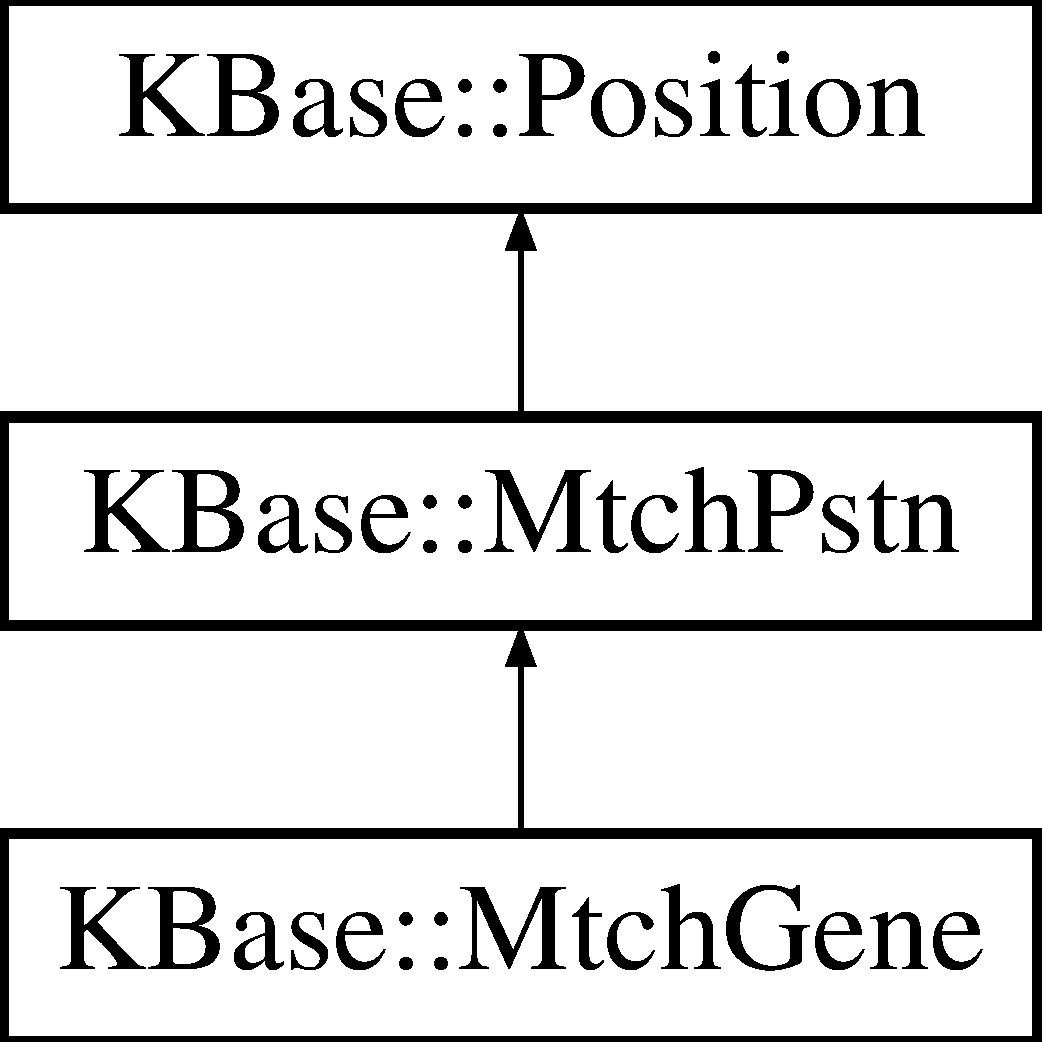
\includegraphics[height=3.000000cm]{class_k_base_1_1_mtch_pstn}
\end{center}
\end{figure}
\subsection*{Public Member Functions}
\begin{DoxyCompactItemize}
\item 
\hypertarget{class_k_base_1_1_mtch_pstn_ad61e5928faa5ba280d1c838e6136ad5d}{virtual vector$<$ \hyperlink{class_k_base_1_1_mtch_pstn}{Mtch\-Pstn} $>$ {\bfseries neighbors} (unsigned int n\-Var) const }\label{class_k_base_1_1_mtch_pstn_ad61e5928faa5ba280d1c838e6136ad5d}

\end{DoxyCompactItemize}
\subsection*{Public Attributes}
\begin{DoxyCompactItemize}
\item 
\hypertarget{class_k_base_1_1_mtch_pstn_a60aa0c0f6712782c4ff8f5990784667c}{unsigned int {\bfseries num\-Itm} = 0}\label{class_k_base_1_1_mtch_pstn_a60aa0c0f6712782c4ff8f5990784667c}

\item 
\hypertarget{class_k_base_1_1_mtch_pstn_ac73b103e757c1700c16ecf4348859711}{unsigned int {\bfseries num\-Cat} = 0}\label{class_k_base_1_1_mtch_pstn_ac73b103e757c1700c16ecf4348859711}

\item 
\hypertarget{class_k_base_1_1_mtch_pstn_a67f468b2b5b27b2c142a83dbf8495743}{V\-U\-I {\bfseries match} = \{\}}\label{class_k_base_1_1_mtch_pstn_a67f468b2b5b27b2c142a83dbf8495743}

\end{DoxyCompactItemize}
\subsection*{Protected Member Functions}
\begin{DoxyCompactItemize}
\item 
\hypertarget{class_k_base_1_1_mtch_pstn_a6e7b76abf2a809ffdeabf599143f596e}{virtual void {\bfseries print} (ostream \&os) const }\label{class_k_base_1_1_mtch_pstn_a6e7b76abf2a809ffdeabf599143f596e}

\end{DoxyCompactItemize}


The documentation for this class was generated from the following files\-:\begin{DoxyCompactItemize}
\item 
kmodel.\-h\item 
kposition.\-cpp\end{DoxyCompactItemize}

\hypertarget{class_demo_mtch_1_1_mtch_state}{\section{Demo\-Mtch\-:\-:Mtch\-State Class Reference}
\label{class_demo_mtch_1_1_mtch_state}\index{Demo\-Mtch\-::\-Mtch\-State@{Demo\-Mtch\-::\-Mtch\-State}}
}
Inheritance diagram for Demo\-Mtch\-:\-:Mtch\-State\-:\begin{figure}[H]
\begin{center}
\leavevmode
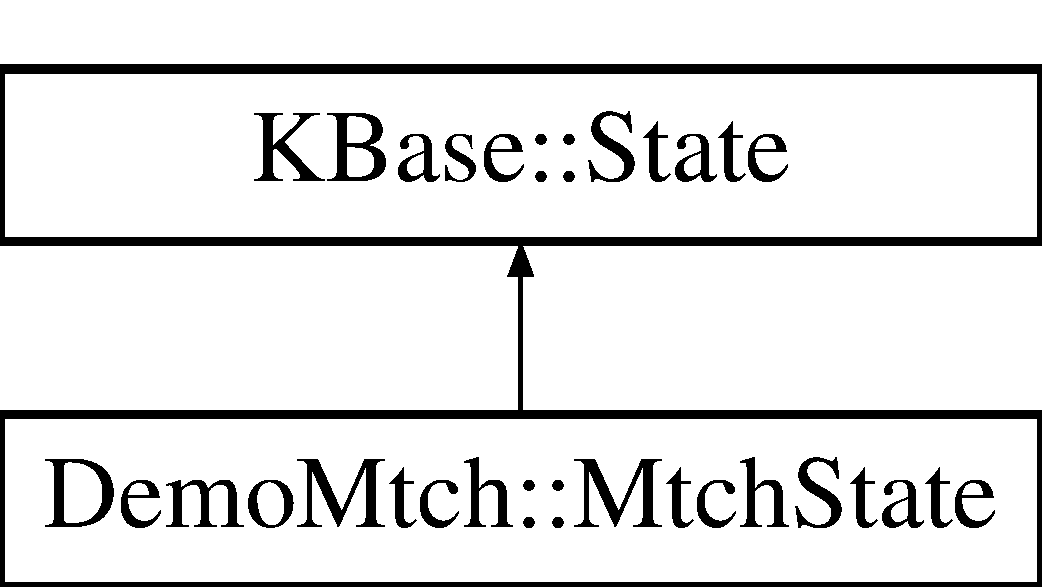
\includegraphics[height=2.000000cm]{class_demo_mtch_1_1_mtch_state}
\end{center}
\end{figure}
\subsection*{Public Member Functions}
\begin{DoxyCompactItemize}
\item 
\hypertarget{class_demo_mtch_1_1_mtch_state_a940ce8e83428691267325da391fd12be}{{\bfseries Mtch\-State} (\hyperlink{class_k_base_1_1_model}{Model} $\ast$mod)}\label{class_demo_mtch_1_1_mtch_state_a940ce8e83428691267325da391fd12be}

\item 
\hypertarget{class_demo_mtch_1_1_mtch_state_a532c2e037446c993b622eba529c6f2c1}{\hyperlink{class_k_base_1_1_k_matrix}{K\-Matrix} {\bfseries actr\-Caps} () const }\label{class_demo_mtch_1_1_mtch_state_a532c2e037446c993b622eba529c6f2c1}

\item 
\hypertarget{class_demo_mtch_1_1_mtch_state_a68cc7caf8632a79c446d6762071adbf6}{tuple$<$ \hyperlink{class_k_base_1_1_k_matrix}{K\-Matrix}, V\-U\-I $>$ {\bfseries p\-Dist} (int persp) const }\label{class_demo_mtch_1_1_mtch_state_a68cc7caf8632a79c446d6762071adbf6}

\item 
\hypertarget{class_demo_mtch_1_1_mtch_state_acce55c8644a16a43ca7c1a82d48ad3e4}{\hyperlink{class_demo_mtch_1_1_mtch_state}{Mtch\-State} $\ast$ {\bfseries step\-S\-U\-S\-N} ()}\label{class_demo_mtch_1_1_mtch_state_acce55c8644a16a43ca7c1a82d48ad3e4}

\item 
\hypertarget{class_demo_mtch_1_1_mtch_state_ac7ce139b487b08c57af543620434877a}{\hyperlink{class_demo_mtch_1_1_mtch_state}{Mtch\-State} $\ast$ {\bfseries step\-B\-C\-N} ()}\label{class_demo_mtch_1_1_mtch_state_ac7ce139b487b08c57af543620434877a}

\end{DoxyCompactItemize}
\subsection*{Protected Member Functions}
\begin{DoxyCompactItemize}
\item 
\hypertarget{class_demo_mtch_1_1_mtch_state_a6891610ea1163e499be356f33afbcd43}{\hyperlink{class_demo_mtch_1_1_mtch_state}{Mtch\-State} $\ast$ {\bfseries do\-S\-U\-S\-N} (Reporting\-Level rl) const }\label{class_demo_mtch_1_1_mtch_state_a6891610ea1163e499be356f33afbcd43}

\item 
\hypertarget{class_demo_mtch_1_1_mtch_state_a9797b5d234245847010e203b83d477a9}{\hyperlink{class_demo_mtch_1_1_mtch_state}{Mtch\-State} $\ast$ {\bfseries do\-B\-C\-N} (Reporting\-Level rl) const }\label{class_demo_mtch_1_1_mtch_state_a9797b5d234245847010e203b83d477a9}

\item 
\hypertarget{class_demo_mtch_1_1_mtch_state_a700815acdb09c6c6b128f1a6cfe6216d}{bool {\bfseries equiv\-Ndx} (unsigned int i, unsigned int j) const }\label{class_demo_mtch_1_1_mtch_state_a700815acdb09c6c6b128f1a6cfe6216d}

\item 
\hypertarget{class_demo_mtch_1_1_mtch_state_af6136ac501980dde51981997ef5cdaec}{void {\bfseries set\-All\-A\-Util} (Reporting\-Level rl)}\label{class_demo_mtch_1_1_mtch_state_af6136ac501980dde51981997ef5cdaec}

\end{DoxyCompactItemize}
\subsection*{Additional Inherited Members}


The documentation for this class was generated from the following files\-:\begin{DoxyCompactItemize}
\item 
demomtch.\-h\item 
demomtch.\-cpp\end{DoxyCompactItemize}

\hypertarget{class_k_graph_1_1_picture}{\section{K\-Graph\-:\-:Picture Class Reference}
\label{class_k_graph_1_1_picture}\index{K\-Graph\-::\-Picture@{K\-Graph\-::\-Picture}}
}
Inheritance diagram for K\-Graph\-:\-:Picture\-:\begin{figure}[H]
\begin{center}
\leavevmode
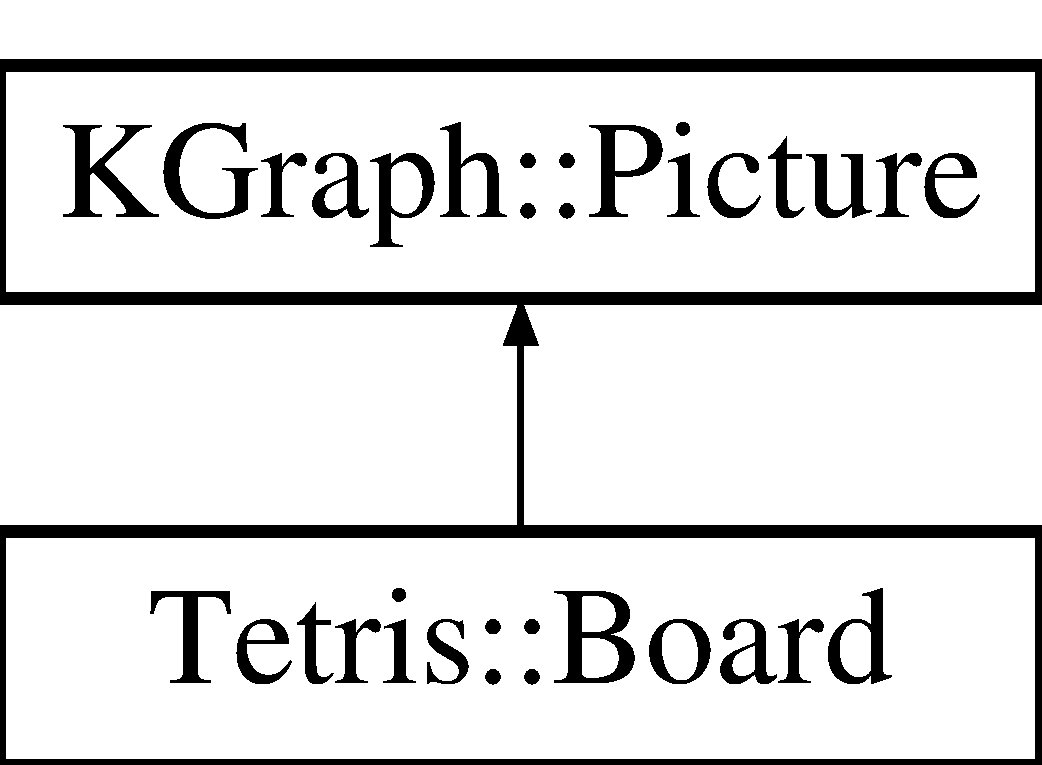
\includegraphics[height=2.000000cm]{class_k_graph_1_1_picture}
\end{center}
\end{figure}
\subsection*{Public Member Functions}
\begin{DoxyCompactItemize}
\item 
\hypertarget{class_k_graph_1_1_picture_a62c483ebdc92a21f0471b815abd95a5c}{void {\bfseries add} (\hyperlink{class_k_graph_1_1_canvas}{Canvas} $\ast$c)}\label{class_k_graph_1_1_picture_a62c483ebdc92a21f0471b815abd95a5c}

\item 
\hypertarget{class_k_graph_1_1_picture_ac6a78e02007c853c4b72ea69b1d8b083}{void {\bfseries update} () const }\label{class_k_graph_1_1_picture_ac6a78e02007c853c4b72ea69b1d8b083}

\item 
\hypertarget{class_k_graph_1_1_picture_ade43b95aa8432929c790bfab6360648c}{virtual void {\bfseries connect} (\hyperlink{class_k_graph_1_1_canvas}{Canvas} $\ast$c)}\label{class_k_graph_1_1_picture_ade43b95aa8432929c790bfab6360648c}

\item 
\hypertarget{class_k_graph_1_1_picture_a9776832c379d30aa59863690c361b1f5}{virtual void {\bfseries update} (\hyperlink{class_k_graph_1_1_canvas}{Canvas} $\ast$c) const }\label{class_k_graph_1_1_picture_a9776832c379d30aa59863690c361b1f5}

\end{DoxyCompactItemize}
\subsection*{Public Attributes}
\begin{DoxyCompactItemize}
\item 
\hypertarget{class_k_graph_1_1_picture_a592b43c93b78d2a5da567275becda80c}{double {\bfseries min\-X} = 0}\label{class_k_graph_1_1_picture_a592b43c93b78d2a5da567275becda80c}

\item 
\hypertarget{class_k_graph_1_1_picture_a4fcdf6e5ba87e59c41d4f5998a3eb2fd}{double {\bfseries max\-X} = 1}\label{class_k_graph_1_1_picture_a4fcdf6e5ba87e59c41d4f5998a3eb2fd}

\item 
\hypertarget{class_k_graph_1_1_picture_a22212d24cf564764d48bfbedab8a2db8}{double {\bfseries min\-W} = 1\-E-\/6}\label{class_k_graph_1_1_picture_a22212d24cf564764d48bfbedab8a2db8}

\item 
\hypertarget{class_k_graph_1_1_picture_adb02963e33c857b45f888cdc8f32359b}{double {\bfseries min\-Y} = 0}\label{class_k_graph_1_1_picture_adb02963e33c857b45f888cdc8f32359b}

\item 
\hypertarget{class_k_graph_1_1_picture_a3f559368c3b1e46bd827e45122a2aa94}{double {\bfseries max\-Y} = 1}\label{class_k_graph_1_1_picture_a3f559368c3b1e46bd827e45122a2aa94}

\item 
\hypertarget{class_k_graph_1_1_picture_a55f1e17679bfbf74fcb70eebdf2fb962}{double {\bfseries min\-H} = 1\-E-\/6}\label{class_k_graph_1_1_picture_a55f1e17679bfbf74fcb70eebdf2fb962}

\end{DoxyCompactItemize}
\subsection*{Protected Attributes}
\begin{DoxyCompactItemize}
\item 
\hypertarget{class_k_graph_1_1_picture_a1feeffcd79f68000918a66972dcfe9e9}{vector$<$ \hyperlink{class_k_graph_1_1_canvas}{Canvas} $\ast$ $>$ {\bfseries canvases} = \{\}}\label{class_k_graph_1_1_picture_a1feeffcd79f68000918a66972dcfe9e9}

\end{DoxyCompactItemize}


The documentation for this class was generated from the following files\-:\begin{DoxyCompactItemize}
\item 
kgraph.\-h\item 
kgraph.\-cpp\end{DoxyCompactItemize}

\hypertarget{class_k_base_1_1_position}{\section{K\-Base\-:\-:Position Class Reference}
\label{class_k_base_1_1_position}\index{K\-Base\-::\-Position@{K\-Base\-::\-Position}}
}
Inheritance diagram for K\-Base\-:\-:Position\-:\begin{figure}[H]
\begin{center}
\leavevmode
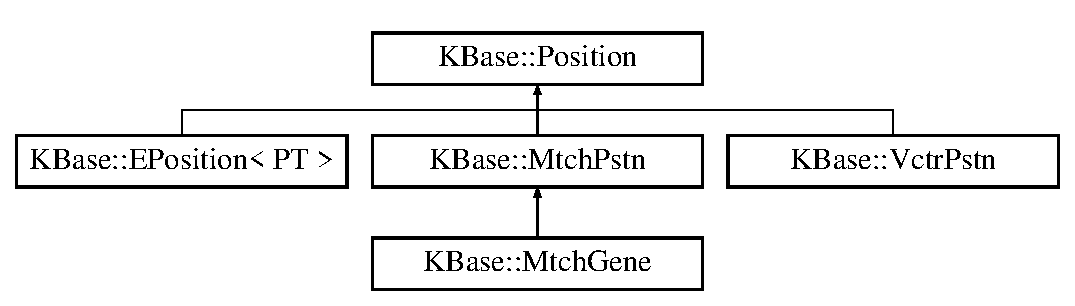
\includegraphics[height=3.000000cm]{class_k_base_1_1_position}
\end{center}
\end{figure}
\subsection*{Protected Member Functions}
\begin{DoxyCompactItemize}
\item 
\hypertarget{class_k_base_1_1_position_a4ae09e7209a5d0caeb51f1c977a21824}{virtual void {\bfseries print} (ostream \&os) const =0}\label{class_k_base_1_1_position_a4ae09e7209a5d0caeb51f1c977a21824}

\end{DoxyCompactItemize}
\subsection*{Friends}
\begin{DoxyCompactItemize}
\item 
\hypertarget{class_k_base_1_1_position_ab7b251ca32003b3e085beb58f406e9ce}{ostream \& {\bfseries operator$<$$<$} (ostream \&os, const \hyperlink{class_k_base_1_1_position}{Position} \&p)}\label{class_k_base_1_1_position_ab7b251ca32003b3e085beb58f406e9ce}

\end{DoxyCompactItemize}


The documentation for this class was generated from the following files\-:\begin{DoxyCompactItemize}
\item 
kmodel.\-h\item 
kposition.\-cpp\end{DoxyCompactItemize}

\hypertarget{class_k_base_1_1_p_r_n_g}{\section{K\-Base\-:\-:P\-R\-N\-G Class Reference}
\label{class_k_base_1_1_p_r_n_g}\index{K\-Base\-::\-P\-R\-N\-G@{K\-Base\-::\-P\-R\-N\-G}}
}
\subsection*{Public Member Functions}
\begin{DoxyCompactItemize}
\item 
\hypertarget{class_k_base_1_1_p_r_n_g_a46dc1e92993bc3f5c13717a2ea892cb9}{uint64\-\_\-t {\bfseries uniform} ()}\label{class_k_base_1_1_p_r_n_g_a46dc1e92993bc3f5c13717a2ea892cb9}

\item 
\hypertarget{class_k_base_1_1_p_r_n_g_a3d5cc2e611dd7d8c01b84b84be8fd8cf}{double {\bfseries uniform} (double a, double b)}\label{class_k_base_1_1_p_r_n_g_a3d5cc2e611dd7d8c01b84b84be8fd8cf}

\item 
\hypertarget{class_k_base_1_1_p_r_n_g_a4f2b0457ccf0a77f2ded4145a5a61a5e}{vector$<$ bool $>$ {\bfseries bits} (unsigned int nb)}\label{class_k_base_1_1_p_r_n_g_a4f2b0457ccf0a77f2ded4145a5a61a5e}

\item 
\hypertarget{class_k_base_1_1_p_r_n_g_aff129c81bc60399b82f59ff9334cc9f8}{uint64\-\_\-t {\bfseries set\-Seed} (uint64\-\_\-t)}\label{class_k_base_1_1_p_r_n_g_aff129c81bc60399b82f59ff9334cc9f8}

\end{DoxyCompactItemize}
\subsection*{Protected Attributes}
\begin{DoxyCompactItemize}
\item 
\hypertarget{class_k_base_1_1_p_r_n_g_ad5ed2c89c06f6b8d67e978da66f7cdfe}{mt19937\-\_\-64 {\bfseries mt} = mt19937\-\_\-64()}\label{class_k_base_1_1_p_r_n_g_ad5ed2c89c06f6b8d67e978da66f7cdfe}

\end{DoxyCompactItemize}


The documentation for this class was generated from the following files\-:\begin{DoxyCompactItemize}
\item 
prng.\-h\item 
prng.\-cpp\end{DoxyCompactItemize}

\hypertarget{class_tetris_1_1_p_v_canvas}{\section{Tetris\-:\-:P\-V\-Canvas Class Reference}
\label{class_tetris_1_1_p_v_canvas}\index{Tetris\-::\-P\-V\-Canvas@{Tetris\-::\-P\-V\-Canvas}}
}
Inheritance diagram for Tetris\-:\-:P\-V\-Canvas\-:\begin{figure}[H]
\begin{center}
\leavevmode
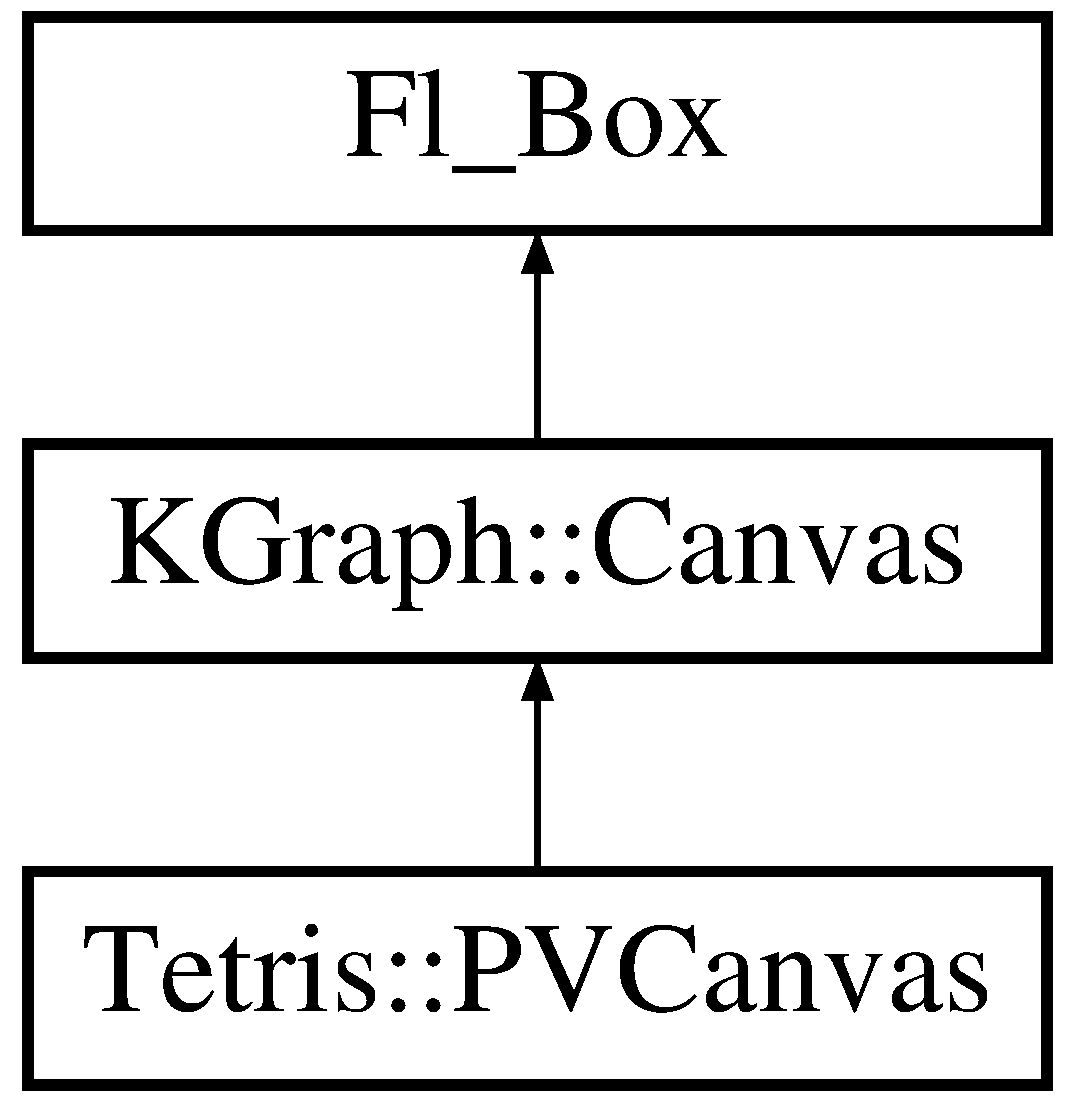
\includegraphics[height=3.000000cm]{class_tetris_1_1_p_v_canvas}
\end{center}
\end{figure}
\subsection*{Public Member Functions}
\begin{DoxyCompactItemize}
\item 
\hypertarget{class_tetris_1_1_p_v_canvas_a9fc62c4882cdf73d03ade0afbdce6077}{{\bfseries P\-V\-Canvas} (int x, int y, int w, int h, const char $\ast$l=0)}\label{class_tetris_1_1_p_v_canvas_a9fc62c4882cdf73d03ade0afbdce6077}

\item 
\hypertarget{class_tetris_1_1_p_v_canvas_ad9ebde55ff948afe38662c1fe3ff4a31}{void {\bfseries on\-Move} (int x, int y)}\label{class_tetris_1_1_p_v_canvas_ad9ebde55ff948afe38662c1fe3ff4a31}

\item 
\hypertarget{class_tetris_1_1_p_v_canvas_a4dd4477abfb914f2d6fb064560a4caa4}{void {\bfseries on\-Drag} (int x, int y)}\label{class_tetris_1_1_p_v_canvas_a4dd4477abfb914f2d6fb064560a4caa4}

\item 
\hypertarget{class_tetris_1_1_p_v_canvas_af6975af5c1557bd019537a75f1eefb36}{void {\bfseries on\-Push} (int x, int y, int b)}\label{class_tetris_1_1_p_v_canvas_af6975af5c1557bd019537a75f1eefb36}

\item 
\hypertarget{class_tetris_1_1_p_v_canvas_ab141246df93f22486a4326891c93871b}{void {\bfseries on\-Release} (int x, int y, int b)}\label{class_tetris_1_1_p_v_canvas_ab141246df93f22486a4326891c93871b}

\item 
\hypertarget{class_tetris_1_1_p_v_canvas_a501b61a67c2b75f1e7095c6552f29e8a}{void {\bfseries on\-Key\-Down} (int x, int y, int k)}\label{class_tetris_1_1_p_v_canvas_a501b61a67c2b75f1e7095c6552f29e8a}

\end{DoxyCompactItemize}
\subsection*{Protected Member Functions}
\begin{DoxyCompactItemize}
\item 
\hypertarget{class_tetris_1_1_p_v_canvas_a21a1d93c93abf96fdcf8421896663c6a}{virtual void {\bfseries draw} ()}\label{class_tetris_1_1_p_v_canvas_a21a1d93c93abf96fdcf8421896663c6a}

\end{DoxyCompactItemize}
\subsection*{Additional Inherited Members}


The documentation for this class was generated from the following files\-:\begin{DoxyCompactItemize}
\item 
pvcanvas.\-h\item 
pvcanvas.\-cpp\end{DoxyCompactItemize}

\hypertarget{class_tetris_1_1_shape}{\section{Tetris\-:\-:Shape Class Reference}
\label{class_tetris_1_1_shape}\index{Tetris\-::\-Shape@{Tetris\-::\-Shape}}
}
\subsection*{Public Member Functions}
\begin{DoxyCompactItemize}
\item 
\hypertarget{class_tetris_1_1_shape_ab85bdb3dde6cbbb1285d1ac1aba6c703}{{\bfseries Shape} (T\-Code p)}\label{class_tetris_1_1_shape_ab85bdb3dde6cbbb1285d1ac1aba6c703}

\item 
\hypertarget{class_tetris_1_1_shape_ac5b889fb9ef82dbd5ab3f7cb7b1dfa6b}{void {\bfseries set\-Shape} (T\-Code p)}\label{class_tetris_1_1_shape_ac5b889fb9ef82dbd5ab3f7cb7b1dfa6b}

\item 
\hypertarget{class_tetris_1_1_shape_aa9ad475137695560851d5870c30ac908}{void {\bfseries set\-Random\-Shape} ()}\label{class_tetris_1_1_shape_aa9ad475137695560851d5870c30ac908}

\item 
\hypertarget{class_tetris_1_1_shape_ae02ede9ddc9bb984ad9a66e662a8c552}{T\-Code {\bfseries get\-Shape} () const }\label{class_tetris_1_1_shape_ae02ede9ddc9bb984ad9a66e662a8c552}

\item 
\hypertarget{class_tetris_1_1_shape_ad88cabd968f4726a8000078c25a5d94f}{char {\bfseries get\-Name} () const }\label{class_tetris_1_1_shape_ad88cabd968f4726a8000078c25a5d94f}

\item 
\hypertarget{class_tetris_1_1_shape_ad3553d75158dfee272012721c9b31c1a}{int {\bfseries x} (int index) const }\label{class_tetris_1_1_shape_ad3553d75158dfee272012721c9b31c1a}

\item 
\hypertarget{class_tetris_1_1_shape_aec2eec106dc13cb887d8e589d12648ab}{int {\bfseries y} (int index) const }\label{class_tetris_1_1_shape_aec2eec106dc13cb887d8e589d12648ab}

\item 
\hypertarget{class_tetris_1_1_shape_a916d65e92ad9bbca5257eed86446efc4}{int {\bfseries min\-X} () const }\label{class_tetris_1_1_shape_a916d65e92ad9bbca5257eed86446efc4}

\item 
\hypertarget{class_tetris_1_1_shape_a507b2c15c9da137051b579237b3348da}{int {\bfseries max\-X} () const }\label{class_tetris_1_1_shape_a507b2c15c9da137051b579237b3348da}

\item 
\hypertarget{class_tetris_1_1_shape_aa227cd9cb83465ae58b69f2c9bf6d9ef}{int {\bfseries min\-Y} () const }\label{class_tetris_1_1_shape_aa227cd9cb83465ae58b69f2c9bf6d9ef}

\item 
\hypertarget{class_tetris_1_1_shape_a0dd5e0b4b728b3a1e02ba381d90e7a3b}{int {\bfseries max\-Y} () const }\label{class_tetris_1_1_shape_a0dd5e0b4b728b3a1e02ba381d90e7a3b}

\item 
\hypertarget{class_tetris_1_1_shape_a9126ac01d08475dfe729ae04d4429be5}{void {\bfseries show\-Coords} () const }\label{class_tetris_1_1_shape_a9126ac01d08475dfe729ae04d4429be5}

\item 
\hypertarget{class_tetris_1_1_shape_ada25de7eeb1d206f41f484338ca6a3cd}{\hyperlink{class_tetris_1_1_shape}{Shape} {\bfseries lrot} () const }\label{class_tetris_1_1_shape_ada25de7eeb1d206f41f484338ca6a3cd}

\item 
\hypertarget{class_tetris_1_1_shape_aff2bb67d1bf30f8398fd670e8a0da0a2}{\hyperlink{class_tetris_1_1_shape}{Shape} {\bfseries rrot} () const }\label{class_tetris_1_1_shape_aff2bb67d1bf30f8398fd670e8a0da0a2}

\end{DoxyCompactItemize}
\subsection*{Public Attributes}
\begin{DoxyCompactItemize}
\item 
\hypertarget{class_tetris_1_1_shape_af7522c63b46b405a89b9975d8c9c8792}{unsigned int {\bfseries id\-Num} = 0}\label{class_tetris_1_1_shape_af7522c63b46b405a89b9975d8c9c8792}

\end{DoxyCompactItemize}
\subsection*{Static Public Attributes}
\begin{DoxyCompactItemize}
\item 
\hypertarget{class_tetris_1_1_shape_adba48f3c02a4226d8a8260d246013658}{static unsigned int {\bfseries shape\-Counter} = 0}\label{class_tetris_1_1_shape_adba48f3c02a4226d8a8260d246013658}

\end{DoxyCompactItemize}


The documentation for this class was generated from the following files\-:\begin{DoxyCompactItemize}
\item 
shape.\-h\item 
shape.\-cpp\end{DoxyCompactItemize}

\hypertarget{class_m_demo_1_1_s_q_l_d_b}{\section{M\-Demo\-:\-:S\-Q\-L\-D\-B Class Reference}
\label{class_m_demo_1_1_s_q_l_d_b}\index{M\-Demo\-::\-S\-Q\-L\-D\-B@{M\-Demo\-::\-S\-Q\-L\-D\-B}}
}
\subsection*{Public Member Functions}
\begin{DoxyCompactItemize}
\item 
\hypertarget{class_m_demo_1_1_s_q_l_d_b_ae7b1ed56a1e8b3d5a187dd6babdbecb6}{{\bfseries S\-Q\-L\-D\-B} (char $\ast$filename)}\label{class_m_demo_1_1_s_q_l_d_b_ae7b1ed56a1e8b3d5a187dd6babdbecb6}

\item 
\hypertarget{class_m_demo_1_1_s_q_l_d_b_afa64d2208de7574486c8b4144d43eda1}{bool {\bfseries open} (char $\ast$filename)}\label{class_m_demo_1_1_s_q_l_d_b_afa64d2208de7574486c8b4144d43eda1}

\item 
\hypertarget{class_m_demo_1_1_s_q_l_d_b_a70dd8fe9e049c6738535aeabec137270}{tuple$<$ unsigned int, vector\\*
$<$ vector$<$ string $>$ $>$ $>$ {\bfseries query} (const char $\ast$query)}\label{class_m_demo_1_1_s_q_l_d_b_a70dd8fe9e049c6738535aeabec137270}

\item 
\hypertarget{class_m_demo_1_1_s_q_l_d_b_a1e13c003c5da5b5851ce4df7bb666d19}{void {\bfseries close} ()}\label{class_m_demo_1_1_s_q_l_d_b_a1e13c003c5da5b5851ce4df7bb666d19}

\end{DoxyCompactItemize}


The documentation for this class was generated from the following files\-:\begin{DoxyCompactItemize}
\item 
sqlitedemo.\-h\item 
sqlitedemo.\-cpp\end{DoxyCompactItemize}

\hypertarget{class_k_base_1_1_state}{\section{K\-Base\-:\-:State Class Reference}
\label{class_k_base_1_1_state}\index{K\-Base\-::\-State@{K\-Base\-::\-State}}
}
Inheritance diagram for K\-Base\-:\-:State\-:\begin{figure}[H]
\begin{center}
\leavevmode
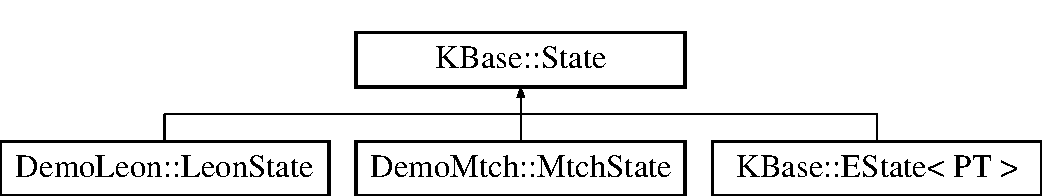
\includegraphics[height=2.000000cm]{class_k_base_1_1_state}
\end{center}
\end{figure}
\subsection*{Public Member Functions}
\begin{DoxyCompactItemize}
\item 
\hypertarget{class_k_base_1_1_state_a3df4aff41e3a45a940118eb3b5eb9e7f}{{\bfseries State} (\hyperlink{class_k_base_1_1_model}{Model} $\ast$mod)}\label{class_k_base_1_1_state_a3df4aff41e3a45a940118eb3b5eb9e7f}

\item 
\hypertarget{class_k_base_1_1_state_a707cd5aa36380ed9857006f1bd94ac82}{void {\bfseries randomize\-Utils} (double min\-U, double max\-U, double u\-Noise)}\label{class_k_base_1_1_state_a707cd5aa36380ed9857006f1bd94ac82}

\item 
\hypertarget{class_k_base_1_1_state_abbe1359b24e0bb85f3864b263642d7c7}{void {\bfseries clear} ()}\label{class_k_base_1_1_state_abbe1359b24e0bb85f3864b263642d7c7}

\item 
\hypertarget{class_k_base_1_1_state_ae2ca6cade9e2eebc0ae92f4d538cb7c3}{virtual void {\bfseries add\-Pstn} (\hyperlink{class_k_base_1_1_position}{Position} $\ast$p)}\label{class_k_base_1_1_state_ae2ca6cade9e2eebc0ae92f4d538cb7c3}

\item 
\hypertarget{class_k_base_1_1_state_ad0b47f5cba11043c02d16a6a51819c02}{virtual tuple$<$ \hyperlink{class_k_base_1_1_k_matrix}{K\-Matrix}, V\-U\-I $>$ {\bfseries p\-Dist} (int persp) const =0}\label{class_k_base_1_1_state_ad0b47f5cba11043c02d16a6a51819c02}

\item 
\hypertarget{class_k_base_1_1_state_a47fa7e79885216bb1bd2185aa54c935e}{void {\bfseries set\-A\-Util} (int persp\-H=-\/1, Reporting\-Level rl=Reporting\-Level\-::\-Silent)}\label{class_k_base_1_1_state_a47fa7e79885216bb1bd2185aa54c935e}

\item 
void \hyperlink{class_k_base_1_1_state_a263291175cbf35293c09784af03a480d}{set\-U\-E\-Ndx} ()
\end{DoxyCompactItemize}
\subsection*{Public Attributes}
\begin{DoxyCompactItemize}
\item 
\hypertarget{class_k_base_1_1_state_a026ba4c3e63a9f7e574f748a43e40161}{\hyperlink{class_k_base_1_1_model}{Model} $\ast$ {\bfseries model} = nullptr}\label{class_k_base_1_1_state_a026ba4c3e63a9f7e574f748a43e40161}

\item 
\hypertarget{class_k_base_1_1_state_a37dd53c90270aceee8c0b873994d1ac7}{function$<$ \hyperlink{class_k_base_1_1_state}{State} $\ast$()$>$ {\bfseries step} = nullptr}\label{class_k_base_1_1_state_a37dd53c90270aceee8c0b873994d1ac7}

\item 
\hypertarget{class_k_base_1_1_state_a574d781488537e4aee8499cb0d31dcfc}{vector$<$ \hyperlink{class_k_base_1_1_position}{Position} $\ast$ $>$ {\bfseries pstns} = \{\}}\label{class_k_base_1_1_state_a574d781488537e4aee8499cb0d31dcfc}

\item 
\hypertarget{class_k_base_1_1_state_a99361c58b6e1351fd621cf16be4d7bb7}{vector$<$ \hyperlink{class_k_base_1_1_k_matrix}{K\-Matrix} $>$ {\bfseries a\-Util} = \{\}}\label{class_k_base_1_1_state_a99361c58b6e1351fd621cf16be4d7bb7}

\end{DoxyCompactItemize}
\subsection*{Protected Member Functions}
\begin{DoxyCompactItemize}
\item 
\hypertarget{class_k_base_1_1_state_a28b1863bc2f9c58e4b83ac33abbb0632}{virtual bool {\bfseries equiv\-Ndx} (unsigned int i, unsigned int j) const =0}\label{class_k_base_1_1_state_a28b1863bc2f9c58e4b83ac33abbb0632}

\item 
\hypertarget{class_k_base_1_1_state_a914af3a6cef478619b59eadb24e00d3c}{virtual void {\bfseries set\-All\-A\-Util} (Reporting\-Level rl)=0}\label{class_k_base_1_1_state_a914af3a6cef478619b59eadb24e00d3c}

\item 
\hypertarget{class_k_base_1_1_state_a5e498c150c69d964de4984c61c41439f}{virtual void {\bfseries set\-One\-A\-Util} (unsigned int persp\-H, Reporting\-Level rl)}\label{class_k_base_1_1_state_a5e498c150c69d964de4984c61c41439f}

\end{DoxyCompactItemize}
\subsection*{Protected Attributes}
\begin{DoxyCompactItemize}
\item 
\hypertarget{class_k_base_1_1_state_a47d133368b216e8a357902cccaec69e1}{V\-U\-I {\bfseries u\-Indices} = \{\}}\label{class_k_base_1_1_state_a47d133368b216e8a357902cccaec69e1}

\item 
\hypertarget{class_k_base_1_1_state_a9c97b8f310790e0546dbe4499dcfdbfa}{V\-U\-I {\bfseries e\-Indices} = \{\}}\label{class_k_base_1_1_state_a9c97b8f310790e0546dbe4499dcfdbfa}

\item 
\hypertarget{class_k_base_1_1_state_a3fb0b1431b94bc82fd45ce9fb8f9fad2}{\hyperlink{class_k_base_1_1_k_matrix}{K\-Matrix} {\bfseries u\-Prob} = \hyperlink{class_k_base_1_1_k_matrix}{K\-Matrix}()}\label{class_k_base_1_1_state_a3fb0b1431b94bc82fd45ce9fb8f9fad2}

\end{DoxyCompactItemize}


\subsection{Member Function Documentation}
\hypertarget{class_k_base_1_1_state_a263291175cbf35293c09784af03a480d}{\index{K\-Base\-::\-State@{K\-Base\-::\-State}!set\-U\-E\-Ndx@{set\-U\-E\-Ndx}}
\index{set\-U\-E\-Ndx@{set\-U\-E\-Ndx}!KBase::State@{K\-Base\-::\-State}}
\subsubsection[{set\-U\-E\-Ndx}]{\setlength{\rightskip}{0pt plus 5cm}void K\-Base\-::\-State\-::set\-U\-E\-Ndx (
\begin{DoxyParamCaption}
{}
\end{DoxyParamCaption}
)}}\label{class_k_base_1_1_state_a263291175cbf35293c09784af03a480d}
Looking only at the positions in this state, return a vector of indices of unique positions. 

The documentation for this class was generated from the following files\-:\begin{DoxyCompactItemize}
\item 
kmodel.\-h\item 
kstate.\-cpp\end{DoxyCompactItemize}

\hypertarget{class_tetris_1_1_t_app}{\section{Tetris\-:\-:T\-App Class Reference}
\label{class_tetris_1_1_t_app}\index{Tetris\-::\-T\-App@{Tetris\-::\-T\-App}}
}
\subsection*{Public Member Functions}
\begin{DoxyCompactItemize}
\item 
\hypertarget{class_tetris_1_1_t_app_a318e10428622a7d949cbb497ef0186a3}{{\bfseries T\-App} (uint64\-\_\-t s)}\label{class_tetris_1_1_t_app_a318e10428622a7d949cbb497ef0186a3}

\item 
\hypertarget{class_tetris_1_1_t_app_a7fb80778823576796323568e0280ff8b}{void {\bfseries run} ()}\label{class_tetris_1_1_t_app_a7fb80778823576796323568e0280ff8b}

\item 
\hypertarget{class_tetris_1_1_t_app_a364fa1df216c28a7434acdbd98409b01}{void {\bfseries new\-Game} ()}\label{class_tetris_1_1_t_app_a364fa1df216c28a7434acdbd98409b01}

\item 
\hypertarget{class_tetris_1_1_t_app_aabca7af9c8e9f50e51222baacb4fc9a4}{void {\bfseries step\-Game} ()}\label{class_tetris_1_1_t_app_aabca7af9c8e9f50e51222baacb4fc9a4}

\item 
\hypertarget{class_tetris_1_1_t_app_a520fc81cbd8b64544fb2cbad9b9e39dd}{void {\bfseries pause} ()}\label{class_tetris_1_1_t_app_a520fc81cbd8b64544fb2cbad9b9e39dd}

\item 
\hypertarget{class_tetris_1_1_t_app_aeb17f1d5b84170d9529fa936f81941da}{void {\bfseries resume} (double delay)}\label{class_tetris_1_1_t_app_aeb17f1d5b84170d9529fa936f81941da}

\item 
\hypertarget{class_tetris_1_1_t_app_ae903c8a96a48c80e33015698f27f3fee}{Fl\-\_\-\-Color {\bfseries color} (unsigned int i) const }\label{class_tetris_1_1_t_app_ae903c8a96a48c80e33015698f27f3fee}

\item 
\hypertarget{class_tetris_1_1_t_app_afd4e1a6f04b9b40d8c4305bbb3cea388}{void {\bfseries set\-R\-C} (unsigned int r, unsigned int c)}\label{class_tetris_1_1_t_app_afd4e1a6f04b9b40d8c4305bbb3cea388}

\item 
\hypertarget{class_tetris_1_1_t_app_a0b3f834907a9653b39fb90370427ffb0}{void {\bfseries set\-Level} (unsigned int lvl)}\label{class_tetris_1_1_t_app_a0b3f834907a9653b39fb90370427ffb0}

\item 
\hypertarget{class_tetris_1_1_t_app_a1cdc89e6c4a1eb70e4dfa57c29b74de3}{void {\bfseries set\-Random} (bool rp)}\label{class_tetris_1_1_t_app_a1cdc89e6c4a1eb70e4dfa57c29b74de3}

\item 
double \hyperlink{class_tetris_1_1_t_app_ad605444e3c0e493fbe2adf1931716cb2}{set\-Dt} ()
\item 
\hypertarget{class_tetris_1_1_t_app_adf8df4d6f560817b5011622e44f4df1c}{void {\bfseries apply\-Control\-State} (\hyperlink{class_tetris_1_1_control_state}{Control\-State} cs)}\label{class_tetris_1_1_t_app_adf8df4d6f560817b5011622e44f4df1c}

\item 
\hypertarget{class_tetris_1_1_t_app_a732575e3dc270b6028f437dbab2e0ab3}{void {\bfseries apply\-Color\-Scheme} (\hyperlink{class_tetris_1_1_control_state}{Control\-State} cs)}\label{class_tetris_1_1_t_app_a732575e3dc270b6028f437dbab2e0ab3}

\item 
\hypertarget{class_tetris_1_1_t_app_a3bacf19e58de8451f045bdf597c61661}{void {\bfseries process\-Key} (int x, int y, int k)}\label{class_tetris_1_1_t_app_a3bacf19e58de8451f045bdf597c61661}

\item 
\hypertarget{class_tetris_1_1_t_app_adf398044bf804163181d7cd1c6c6d482}{void {\bfseries quit} ()}\label{class_tetris_1_1_t_app_adf398044bf804163181d7cd1c6c6d482}

\end{DoxyCompactItemize}
\subsection*{Public Attributes}
\begin{DoxyCompactItemize}
\item 
\hypertarget{class_tetris_1_1_t_app_a5e77231d3cf8221ff138384be0b02d18}{unsigned int {\bfseries level} = 3}\label{class_tetris_1_1_t_app_a5e77231d3cf8221ff138384be0b02d18}

\item 
\hypertarget{class_tetris_1_1_t_app_ae6407e85fa4ef4fb4430c8cf57f4c2f6}{double {\bfseries dt} = 0.\-1}\label{class_tetris_1_1_t_app_ae6407e85fa4ef4fb4430c8cf57f4c2f6}

\item 
\hypertarget{class_tetris_1_1_t_app_a4214c60726ce1689fdf4870c004913b1}{\hyperlink{class_k_base_1_1_p_r_n_g}{P\-R\-N\-G} $\ast$ {\bfseries rng} = nullptr}\label{class_tetris_1_1_t_app_a4214c60726ce1689fdf4870c004913b1}

\item 
\hypertarget{class_tetris_1_1_t_app_aff7fbc6c4c5f0cdcb5597cca285e9363}{\hyperlink{class_tetris_1_1_board}{Board} $\ast$ {\bfseries board} = nullptr}\label{class_tetris_1_1_t_app_aff7fbc6c4c5f0cdcb5597cca285e9363}

\item 
\hypertarget{class_tetris_1_1_t_app_ac1468b74711d7b95bdd4d90887950d8b}{unsigned int {\bfseries rows} = 0}\label{class_tetris_1_1_t_app_ac1468b74711d7b95bdd4d90887950d8b}

\item 
\hypertarget{class_tetris_1_1_t_app_a0089732349106389c46366cb8814ec3f}{unsigned int {\bfseries clms} = 0}\label{class_tetris_1_1_t_app_a0089732349106389c46366cb8814ec3f}

\item 
\hypertarget{class_tetris_1_1_t_app_add4a992aed9f6df69c264348ce8361c1}{bool {\bfseries random\-Placement} = false}\label{class_tetris_1_1_t_app_add4a992aed9f6df69c264348ce8361c1}

\item 
\hypertarget{class_tetris_1_1_t_app_a0a0b6ecfce8936a68969eb6cbc7d9ff8}{double {\bfseries play\-Time} = 5$\ast$60}\label{class_tetris_1_1_t_app_a0a0b6ecfce8936a68969eb6cbc7d9ff8}

\item 
\hypertarget{class_tetris_1_1_t_app_a762186a8ba125b0ebb35362500b05db2}{double {\bfseries max\-Play\-Time} = 10$\ast$60}\label{class_tetris_1_1_t_app_a762186a8ba125b0ebb35362500b05db2}

\item 
\hypertarget{class_tetris_1_1_t_app_aaeab34b7813c54f2bc20f56919d7dd42}{bool {\bfseries paused} = true}\label{class_tetris_1_1_t_app_aaeab34b7813c54f2bc20f56919d7dd42}

\end{DoxyCompactItemize}
\subsection*{Static Public Attributes}
\begin{DoxyCompactItemize}
\item 
\hypertarget{class_tetris_1_1_t_app_a4094b827652596527f51beb466db5d68}{static \hyperlink{class_tetris_1_1_t_app}{T\-App} $\ast$ {\bfseries the\-App} = nullptr}\label{class_tetris_1_1_t_app_a4094b827652596527f51beb466db5d68}

\end{DoxyCompactItemize}
\subsection*{Protected Member Functions}
\begin{DoxyCompactItemize}
\item 
\hypertarget{class_tetris_1_1_t_app_a6858685050efe4d337b8dced7d7ada8c}{unsigned int {\bfseries score\-Fn} (unsigned int clc)}\label{class_tetris_1_1_t_app_a6858685050efe4d337b8dced7d7ada8c}

\item 
\hypertarget{class_tetris_1_1_t_app_a8bad5ebd128c393ae2ea78c3be1100ec}{void {\bfseries set\-Color\-Scheme} ()}\label{class_tetris_1_1_t_app_a8bad5ebd128c393ae2ea78c3be1100ec}

\end{DoxyCompactItemize}
\subsection*{Protected Attributes}
\begin{DoxyCompactItemize}
\item 
\hypertarget{class_tetris_1_1_t_app_affa00d5962fc8acaa590144ef148ea3b}{unsigned int {\bfseries line\-Count} = 0}\label{class_tetris_1_1_t_app_affa00d5962fc8acaa590144ef148ea3b}

\item 
\hypertarget{class_tetris_1_1_t_app_a2ca1002b0317c05ec00544603812d252}{unsigned int {\bfseries score} = 0}\label{class_tetris_1_1_t_app_a2ca1002b0317c05ec00544603812d252}

\item 
\hypertarget{class_tetris_1_1_t_app_ad8b35f905b6efc76535349c306d6586f}{const unsigned int {\bfseries default\-Level} = 3}\label{class_tetris_1_1_t_app_ad8b35f905b6efc76535349c306d6586f}

\item 
\hypertarget{class_tetris_1_1_t_app_aa6b6f30e4c252d5206c192d34c74dfc0}{const unsigned int {\bfseries default\-Rows} = 24}\label{class_tetris_1_1_t_app_aa6b6f30e4c252d5206c192d34c74dfc0}

\item 
\hypertarget{class_tetris_1_1_t_app_aee50ab6d5aee1c468c9ffdd7f7c1c109}{const unsigned int {\bfseries default\-Clms} = 12}\label{class_tetris_1_1_t_app_aee50ab6d5aee1c468c9ffdd7f7c1c109}

\item 
\hypertarget{class_tetris_1_1_t_app_a04fc4c4c38992ab93ee6166d8ac5822a}{const bool {\bfseries default\-R\-P} = false}\label{class_tetris_1_1_t_app_a04fc4c4c38992ab93ee6166d8ac5822a}

\item 
\hypertarget{class_tetris_1_1_t_app_a9232907654626b70538113c6971cb39f}{vector$<$ Fl\-\_\-\-Color $>$ {\bfseries colors} = \{\}}\label{class_tetris_1_1_t_app_a9232907654626b70538113c6971cb39f}

\end{DoxyCompactItemize}


\subsection{Member Function Documentation}
\hypertarget{class_tetris_1_1_t_app_ad605444e3c0e493fbe2adf1931716cb2}{\index{Tetris\-::\-T\-App@{Tetris\-::\-T\-App}!set\-Dt@{set\-Dt}}
\index{set\-Dt@{set\-Dt}!Tetris::TApp@{Tetris\-::\-T\-App}}
\subsubsection[{set\-Dt}]{\setlength{\rightskip}{0pt plus 5cm}double Tetris\-::\-T\-App\-::set\-Dt (
\begin{DoxyParamCaption}
{}
\end{DoxyParamCaption}
)}}\label{class_tetris_1_1_t_app_ad605444e3c0e493fbe2adf1931716cb2}
set the time between updates, given the current level 

The documentation for this class was generated from the following files\-:\begin{DoxyCompactItemize}
\item 
tmain.\-h\item 
tmain.\-cpp\end{DoxyCompactItemize}

\hypertarget{class_u_demo_1_1_targeted_b_v}{\section{U\-Demo\-:\-:Targeted\-B\-V Class Reference}
\label{class_u_demo_1_1_targeted_b_v}\index{U\-Demo\-::\-Targeted\-B\-V@{U\-Demo\-::\-Targeted\-B\-V}}
}
\subsection*{Public Member Functions}
\begin{DoxyCompactItemize}
\item 
\hypertarget{class_u_demo_1_1_targeted_b_v_a5a9f4b466a1d8c2ec41350fec65e9c31}{virtual void {\bfseries randomize} (\hyperlink{class_k_base_1_1_p_r_n_g}{P\-R\-N\-G} $\ast$rng)}\label{class_u_demo_1_1_targeted_b_v_a5a9f4b466a1d8c2ec41350fec65e9c31}

\item 
\hypertarget{class_u_demo_1_1_targeted_b_v_aa3b7e42fd5ed918d1d4d11b51ab1e434}{virtual \hyperlink{class_u_demo_1_1_targeted_b_v}{Targeted\-B\-V} $\ast$ {\bfseries mutate} (\hyperlink{class_k_base_1_1_p_r_n_g}{P\-R\-N\-G} $\ast$rng) const }\label{class_u_demo_1_1_targeted_b_v_aa3b7e42fd5ed918d1d4d11b51ab1e434}

\item 
\hypertarget{class_u_demo_1_1_targeted_b_v_a0c0fe1016dc3c82dfbfc0c1a2dcaf657}{virtual tuple$<$ \hyperlink{class_u_demo_1_1_targeted_b_v}{Targeted\-B\-V} \\*
$\ast$, \hyperlink{class_u_demo_1_1_targeted_b_v}{Targeted\-B\-V} $\ast$ $>$ {\bfseries cross} (const \hyperlink{class_u_demo_1_1_targeted_b_v}{Targeted\-B\-V} $\ast$g2, \hyperlink{class_k_base_1_1_p_r_n_g}{P\-R\-N\-G} $\ast$rng) const }\label{class_u_demo_1_1_targeted_b_v_a0c0fe1016dc3c82dfbfc0c1a2dcaf657}

\item 
\hypertarget{class_u_demo_1_1_targeted_b_v_af067b5a2d86ecc68dc9c699e88cda892}{virtual void {\bfseries show} () const }\label{class_u_demo_1_1_targeted_b_v_af067b5a2d86ecc68dc9c699e88cda892}

\item 
\hypertarget{class_u_demo_1_1_targeted_b_v_ad4ad679c46e696a7bcd6e14416e14887}{virtual bool {\bfseries equiv} (const \hyperlink{class_u_demo_1_1_targeted_b_v}{Targeted\-B\-V} $\ast$g2) const }\label{class_u_demo_1_1_targeted_b_v_ad4ad679c46e696a7bcd6e14416e14887}

\item 
\hypertarget{class_u_demo_1_1_targeted_b_v_a73d1682bfb09b5aebab8c29baf99c760}{double {\bfseries evaluate} ()}\label{class_u_demo_1_1_targeted_b_v_a73d1682bfb09b5aebab8c29baf99c760}

\item 
\hypertarget{class_u_demo_1_1_targeted_b_v_a5338a3ce60b8731e18ddb44d452521ca}{double {\bfseries tbl\-Eval} (double min\-D, vector$<$ double $>$ weights, vector$<$ B\-Vec $>$ tbl) const }\label{class_u_demo_1_1_targeted_b_v_a5338a3ce60b8731e18ddb44d452521ca}

\item 
\hypertarget{class_u_demo_1_1_targeted_b_v_adb9956e020b7be112720aac52fb6549b}{unsigned int {\bfseries h\-Dist} (B\-Vec bv) const }\label{class_u_demo_1_1_targeted_b_v_adb9956e020b7be112720aac52fb6549b}

\end{DoxyCompactItemize}
\subsection*{Static Public Member Functions}
\begin{DoxyCompactItemize}
\item 
\hypertarget{class_u_demo_1_1_targeted_b_v_a22e7508fcdba461a70451922a2d9ac7d}{static void {\bfseries set\-Target} (B\-Vec trgt)}\label{class_u_demo_1_1_targeted_b_v_a22e7508fcdba461a70451922a2d9ac7d}

\item 
\hypertarget{class_u_demo_1_1_targeted_b_v_adfeab920c07d1618dc126fda84bff621}{static B\-Vec {\bfseries get\-Target} ()}\label{class_u_demo_1_1_targeted_b_v_adfeab920c07d1618dc126fda84bff621}

\item 
\hypertarget{class_u_demo_1_1_targeted_b_v_a71c0f136d7c4ea5c0946b4a889382f24}{static void {\bfseries show\-Bits} (B\-Vec bv)}\label{class_u_demo_1_1_targeted_b_v_a71c0f136d7c4ea5c0946b4a889382f24}

\item 
\hypertarget{class_u_demo_1_1_targeted_b_v_ac5b5aff9e9eaba6e6e6a42f8f6a6b64e}{static B\-Vec {\bfseries random\-B\-V} (\hyperlink{class_k_base_1_1_p_r_n_g}{P\-R\-N\-G} $\ast$rng, unsigned int nb)}\label{class_u_demo_1_1_targeted_b_v_ac5b5aff9e9eaba6e6e6a42f8f6a6b64e}

\end{DoxyCompactItemize}
\subsection*{Public Attributes}
\begin{DoxyCompactItemize}
\item 
\hypertarget{class_u_demo_1_1_targeted_b_v_a9a179eb46b8e30ea2ddf818c1064ef1c}{B\-Vec {\bfseries bits} = B\-Vec()}\label{class_u_demo_1_1_targeted_b_v_a9a179eb46b8e30ea2ddf818c1064ef1c}

\end{DoxyCompactItemize}
\subsection*{Static Public Attributes}
\begin{DoxyCompactItemize}
\item 
\hypertarget{class_u_demo_1_1_targeted_b_v_abad5a7740ce9341652ca284d99634f65}{static B\-Vec {\bfseries target}}\label{class_u_demo_1_1_targeted_b_v_abad5a7740ce9341652ca284d99634f65}

\end{DoxyCompactItemize}


The documentation for this class was generated from the following files\-:\begin{DoxyCompactItemize}
\item 
kutils/src/demo.\-h\item 
kutils/src/demo.\-cpp\end{DoxyCompactItemize}

\hypertarget{class_tetris_1_1_t_canvas}{\section{Tetris\-:\-:T\-Canvas Class Reference}
\label{class_tetris_1_1_t_canvas}\index{Tetris\-::\-T\-Canvas@{Tetris\-::\-T\-Canvas}}
}
Inheritance diagram for Tetris\-:\-:T\-Canvas\-:\begin{figure}[H]
\begin{center}
\leavevmode
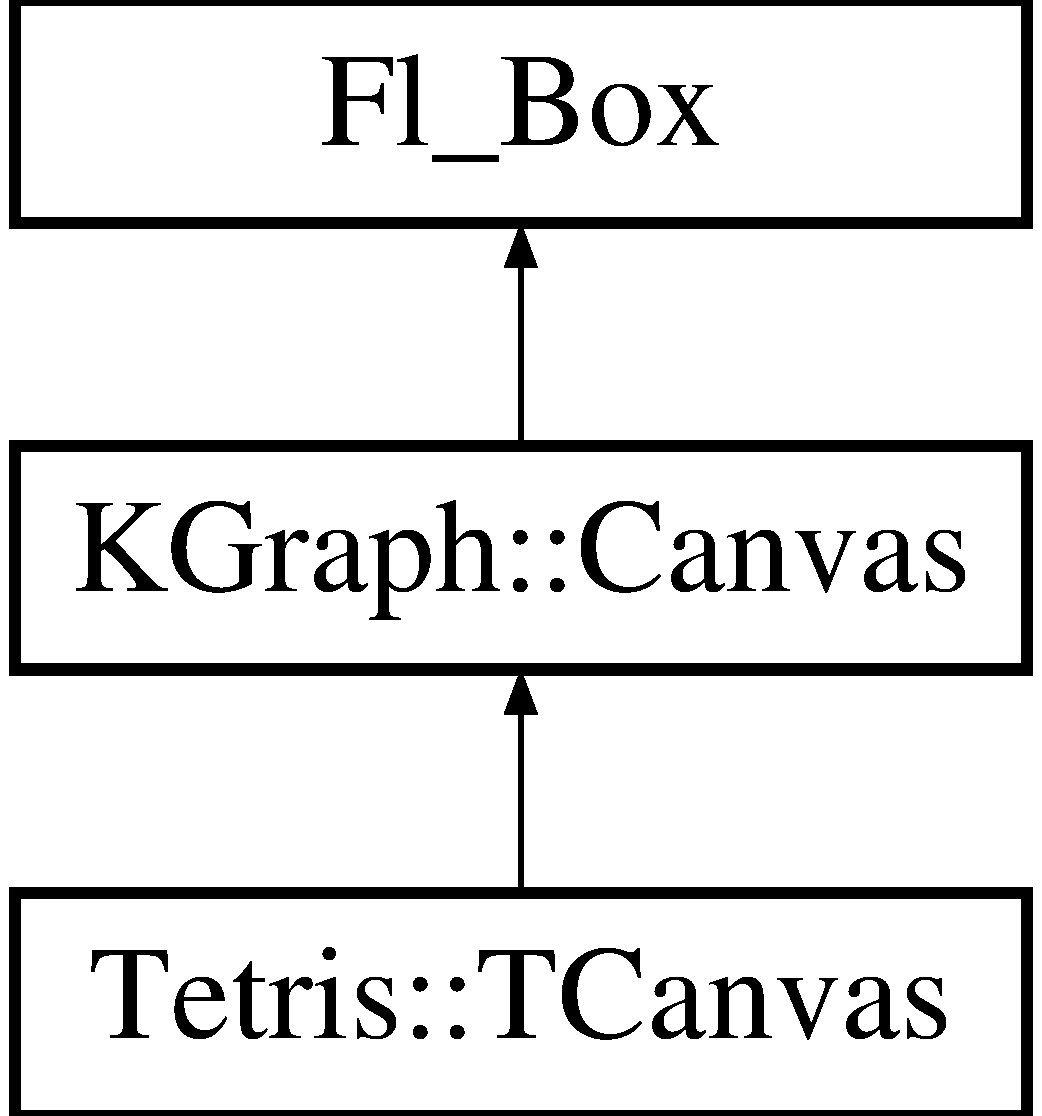
\includegraphics[height=3.000000cm]{class_tetris_1_1_t_canvas}
\end{center}
\end{figure}
\subsection*{Public Member Functions}
\begin{DoxyCompactItemize}
\item 
\hypertarget{class_tetris_1_1_t_canvas_a90791be4bc594cb4892caae0a52648f9}{{\bfseries T\-Canvas} (int x, int y, int w, int h, const char $\ast$l=0)}\label{class_tetris_1_1_t_canvas_a90791be4bc594cb4892caae0a52648f9}

\item 
\hypertarget{class_tetris_1_1_t_canvas_a8b19b8162a434620547de8afb101fc5c}{void {\bfseries on\-Move} (int x, int y)}\label{class_tetris_1_1_t_canvas_a8b19b8162a434620547de8afb101fc5c}

\item 
\hypertarget{class_tetris_1_1_t_canvas_ac43081f6deb9437ebe044cf98e2e6e58}{void {\bfseries on\-Drag} (int x, int y)}\label{class_tetris_1_1_t_canvas_ac43081f6deb9437ebe044cf98e2e6e58}

\item 
\hypertarget{class_tetris_1_1_t_canvas_a5dec34dba9268c77f2fbb2b2ec5df5ad}{void {\bfseries on\-Push} (int x, int y, int b)}\label{class_tetris_1_1_t_canvas_a5dec34dba9268c77f2fbb2b2ec5df5ad}

\item 
\hypertarget{class_tetris_1_1_t_canvas_ad16d10216c737def213b1abe66ab8865}{void {\bfseries on\-Release} (int x, int y, int b)}\label{class_tetris_1_1_t_canvas_ad16d10216c737def213b1abe66ab8865}

\item 
\hypertarget{class_tetris_1_1_t_canvas_a0f4b7e7d02b6168bfd3b25f4afb35eaa}{void {\bfseries on\-Key\-Down} (int x, int y, int k)}\label{class_tetris_1_1_t_canvas_a0f4b7e7d02b6168bfd3b25f4afb35eaa}

\end{DoxyCompactItemize}
\subsection*{Protected Member Functions}
\begin{DoxyCompactItemize}
\item 
\hypertarget{class_tetris_1_1_t_canvas_ad98121011f25b9cabaa78acbc71155d0}{virtual void {\bfseries draw} ()}\label{class_tetris_1_1_t_canvas_ad98121011f25b9cabaa78acbc71155d0}

\end{DoxyCompactItemize}
\subsection*{Additional Inherited Members}


The documentation for this class was generated from the following files\-:\begin{DoxyCompactItemize}
\item 
tcanvas.\-h\item 
tcanvas.\-cpp\end{DoxyCompactItemize}

\hypertarget{struct_m_demo_1_1_two_d_point}{\section{M\-Demo\-:\-:Two\-D\-Point Struct Reference}
\label{struct_m_demo_1_1_two_d_point}\index{M\-Demo\-::\-Two\-D\-Point@{M\-Demo\-::\-Two\-D\-Point}}
}
\subsection*{Public Member Functions}
\begin{DoxyCompactItemize}
\item 
\hypertarget{struct_m_demo_1_1_two_d_point_a78a2a50aa595b6dcf1a6fc2cb09dab4e}{{\bfseries Two\-D\-Point} (unsigned int a, unsigned int b)}\label{struct_m_demo_1_1_two_d_point_a78a2a50aa595b6dcf1a6fc2cb09dab4e}

\end{DoxyCompactItemize}
\subsection*{Public Attributes}
\begin{DoxyCompactItemize}
\item 
\hypertarget{struct_m_demo_1_1_two_d_point_ad505f0b8648c126247913282ab507bb5}{unsigned int {\bfseries x} = 0}\label{struct_m_demo_1_1_two_d_point_ad505f0b8648c126247913282ab507bb5}

\item 
\hypertarget{struct_m_demo_1_1_two_d_point_a19e975e710dad5dcd2f9a31be0c97322}{unsigned int {\bfseries y} = 0}\label{struct_m_demo_1_1_two_d_point_a19e975e710dad5dcd2f9a31be0c97322}

\end{DoxyCompactItemize}


The documentation for this struct was generated from the following files\-:\begin{DoxyCompactItemize}
\item 
edemo.\-h\item 
edemo.\-cpp\end{DoxyCompactItemize}

\hypertarget{class_k_base_1_1_vctr_pstn}{\section{K\-Base\-:\-:Vctr\-Pstn Class Reference}
\label{class_k_base_1_1_vctr_pstn}\index{K\-Base\-::\-Vctr\-Pstn@{K\-Base\-::\-Vctr\-Pstn}}
}
Inheritance diagram for K\-Base\-:\-:Vctr\-Pstn\-:\begin{figure}[H]
\begin{center}
\leavevmode
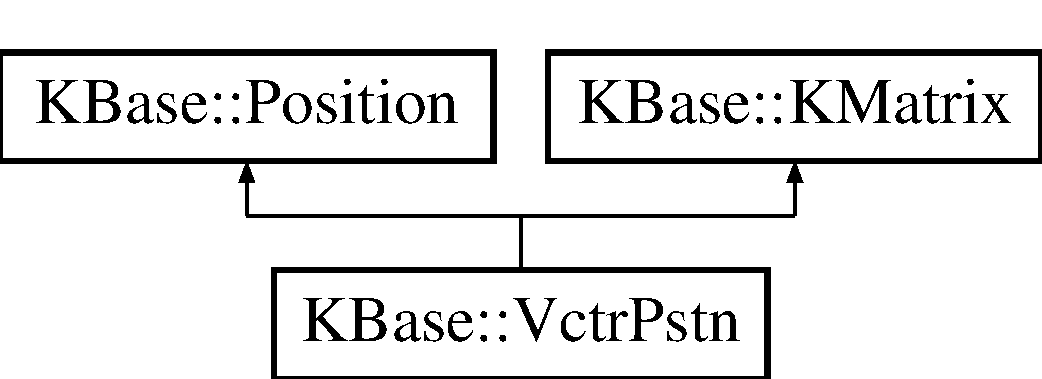
\includegraphics[height=2.000000cm]{class_k_base_1_1_vctr_pstn}
\end{center}
\end{figure}
\subsection*{Public Member Functions}
\begin{DoxyCompactItemize}
\item 
\hypertarget{class_k_base_1_1_vctr_pstn_a662f7ab962cbd356ab2429afc27a7b05}{{\bfseries Vctr\-Pstn} (unsigned int nr, unsigned int nc)}\label{class_k_base_1_1_vctr_pstn_a662f7ab962cbd356ab2429afc27a7b05}

\item 
\hypertarget{class_k_base_1_1_vctr_pstn_ad3e073c7a651c7d69a931cdcbf73586d}{{\bfseries Vctr\-Pstn} (const \hyperlink{class_k_base_1_1_k_matrix}{K\-Matrix} \&m)}\label{class_k_base_1_1_vctr_pstn_ad3e073c7a651c7d69a931cdcbf73586d}

\end{DoxyCompactItemize}
\subsection*{Protected Member Functions}
\begin{DoxyCompactItemize}
\item 
\hypertarget{class_k_base_1_1_vctr_pstn_acf76fb21e89a3a4d12444767562ddca5}{virtual void {\bfseries print} (ostream \&os) const }\label{class_k_base_1_1_vctr_pstn_acf76fb21e89a3a4d12444767562ddca5}

\end{DoxyCompactItemize}
\subsection*{Additional Inherited Members}


The documentation for this class was generated from the following files\-:\begin{DoxyCompactItemize}
\item 
kmodel.\-h\item 
kposition.\-cpp\end{DoxyCompactItemize}

\hypertarget{class_k_base_1_1_v_h_c_search}{\section{K\-Base\-:\-:V\-H\-C\-Search Class Reference}
\label{class_k_base_1_1_v_h_c_search}\index{K\-Base\-::\-V\-H\-C\-Search@{K\-Base\-::\-V\-H\-C\-Search}}
}
\subsection*{Public Member Functions}
\begin{DoxyCompactItemize}
\item 
\hypertarget{class_k_base_1_1_v_h_c_search_a27cd0d24dd198727288211eeda5b22b3}{tuple$<$ double, \hyperlink{class_k_base_1_1_k_matrix}{K\-Matrix}, \\*
unsigned int, unsigned int $>$ {\bfseries run} (\hyperlink{class_k_base_1_1_k_matrix}{K\-Matrix} p0, unsigned int i\-Max, unsigned int s\-Max, double s\-Tol, double s0, double shrink, double grow, double min\-Step, Reporting\-Level rl)}\label{class_k_base_1_1_v_h_c_search_a27cd0d24dd198727288211eeda5b22b3}

\end{DoxyCompactItemize}
\subsection*{Static Public Member Functions}
\begin{DoxyCompactItemize}
\item 
\hypertarget{class_k_base_1_1_v_h_c_search_a7a5a28c62b400f8dedaedeb64a4a2c69}{static vector$<$ \hyperlink{class_k_base_1_1_k_matrix}{K\-Matrix} $>$ {\bfseries vn1} (const \hyperlink{class_k_base_1_1_k_matrix}{K\-Matrix} \&m0, double s)}\label{class_k_base_1_1_v_h_c_search_a7a5a28c62b400f8dedaedeb64a4a2c69}

\item 
\hypertarget{class_k_base_1_1_v_h_c_search_a5bb7ee63beefb06208451d32f57b4079}{static vector$<$ \hyperlink{class_k_base_1_1_k_matrix}{K\-Matrix} $>$ {\bfseries vn2} (const \hyperlink{class_k_base_1_1_k_matrix}{K\-Matrix} \&m0, double s)}\label{class_k_base_1_1_v_h_c_search_a5bb7ee63beefb06208451d32f57b4079}

\end{DoxyCompactItemize}
\subsection*{Public Attributes}
\begin{DoxyCompactItemize}
\item 
\hypertarget{class_k_base_1_1_v_h_c_search_aa21cec8bb60f9045844cb2b227d40d6d}{function$<$ double(const \hyperlink{class_k_base_1_1_k_matrix}{K\-Matrix} \&)$>$ {\bfseries eval} = nullptr}\label{class_k_base_1_1_v_h_c_search_aa21cec8bb60f9045844cb2b227d40d6d}

\item 
\hypertarget{class_k_base_1_1_v_h_c_search_a8d380d740b3d3f1a70f7ffba84e40aa4}{function$<$ vector$<$ \hyperlink{class_k_base_1_1_k_matrix}{K\-Matrix} $>$\\*
const \hyperlink{class_k_base_1_1_k_matrix}{K\-Matrix} \&, double)$>$ {\bfseries nghbrs} = nullptr}\label{class_k_base_1_1_v_h_c_search_a8d380d740b3d3f1a70f7ffba84e40aa4}

\item 
\hypertarget{class_k_base_1_1_v_h_c_search_ac941aad6b2362e53d5dabfb8289c84ae}{function$<$ void(const \hyperlink{class_k_base_1_1_k_matrix}{K\-Matrix} \&)$>$ {\bfseries report} = nullptr}\label{class_k_base_1_1_v_h_c_search_ac941aad6b2362e53d5dabfb8289c84ae}

\end{DoxyCompactItemize}


The documentation for this class was generated from the following files\-:\begin{DoxyCompactItemize}
\item 
hcsearch.\-h\item 
hcsearch.\-cpp\end{DoxyCompactItemize}

\hypertarget{class_m_demo_1_1_z_actor}{\section{M\-Demo\-:\-:Z\-Actor Class Reference}
\label{class_m_demo_1_1_z_actor}\index{M\-Demo\-::\-Z\-Actor@{M\-Demo\-::\-Z\-Actor}}
}
Inheritance diagram for M\-Demo\-:\-:Z\-Actor\-:\begin{figure}[H]
\begin{center}
\leavevmode
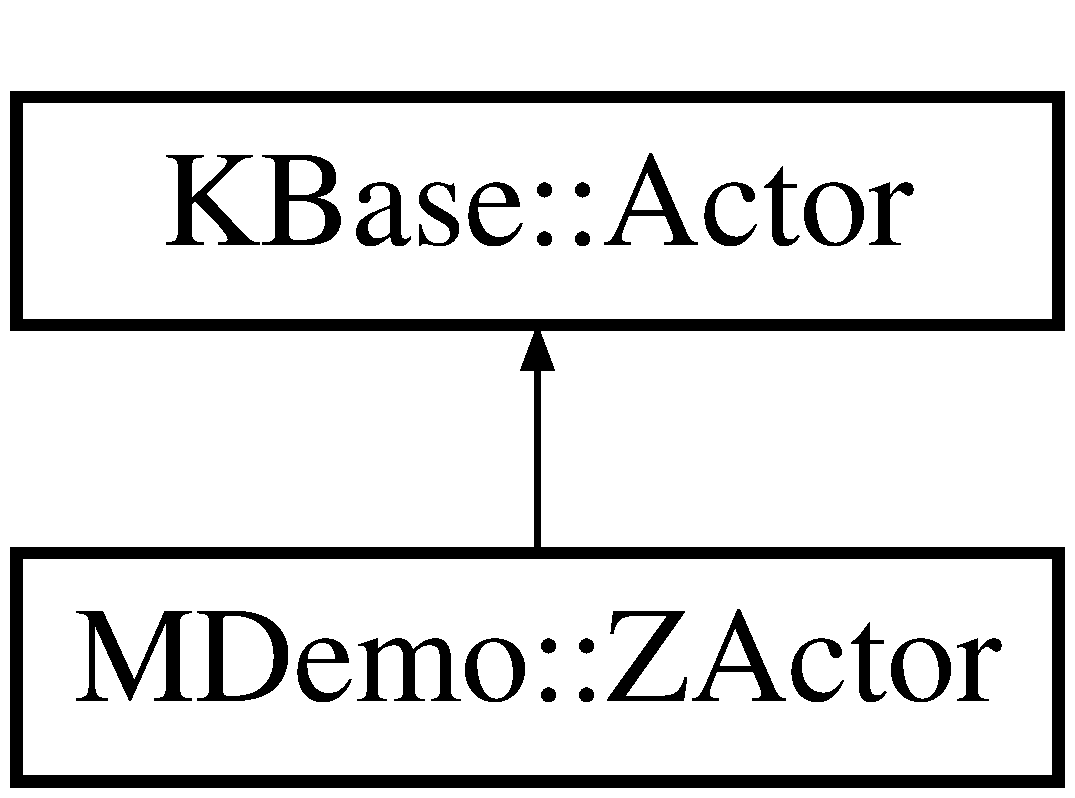
\includegraphics[height=2.000000cm]{class_m_demo_1_1_z_actor}
\end{center}
\end{figure}
\subsection*{Public Member Functions}
\begin{DoxyCompactItemize}
\item 
\hypertarget{class_m_demo_1_1_z_actor_add67a9fe96f4602aa06ccaa68c0f4fc7}{{\bfseries Z\-Actor} (string n, string d)}\label{class_m_demo_1_1_z_actor_add67a9fe96f4602aa06ccaa68c0f4fc7}

\item 
\hypertarget{class_m_demo_1_1_z_actor_ab43b2574f0c915a6752cf35342773163}{double {\bfseries vote} (unsigned int p1, unsigned int p2, const \hyperlink{class_k_base_1_1_state}{State} $\ast$st) const }\label{class_m_demo_1_1_z_actor_ab43b2574f0c915a6752cf35342773163}

\item 
\hypertarget{class_m_demo_1_1_z_actor_a8353eb51f6d09b6111fafa2e8299fa3e}{virtual double {\bfseries vote} (const \hyperlink{class_k_base_1_1_position}{Position} $\ast$ap1, const \hyperlink{class_k_base_1_1_position}{Position} $\ast$ap2) const }\label{class_m_demo_1_1_z_actor_a8353eb51f6d09b6111fafa2e8299fa3e}

\item 
\hypertarget{class_m_demo_1_1_z_actor_a6bd5b6fa4defc8cda93be2c31e40dec9}{double {\bfseries pos\-Util} (const \hyperlink{class_k_base_1_1_position}{Position} $\ast$ap1) const }\label{class_m_demo_1_1_z_actor_a6bd5b6fa4defc8cda93be2c31e40dec9}

\end{DoxyCompactItemize}
\subsection*{Additional Inherited Members}


The documentation for this class was generated from the following files\-:\begin{DoxyCompactItemize}
\item 
zactor.\-h\item 
zactor.\-cpp\end{DoxyCompactItemize}

%--- End generated contents ---

% Index
\newpage
\phantomsection
\addcontentsline{toc}{chapter}{Index}
\printindex

\end{document}
